%% For double-blind review submission, w/o CCS and ACM Reference (max submission space)
%\documentclass[sigplan,10pt,review,anonymous]{acmart}
%\settopmatter{printfolios=false,printccs=false,printacmref=false}
%% For double-blind review submission, w/ CCS and ACM Reference
%\documentclass[sigplan,review,anonymous]{acmart}\settopmatter{printfolios=true}
%% For single-blind review submission, w/o CCS and ACM Reference (max submission space)
%\documentclass[sigplan,review]{acmart}\settopmatter{printfolios=true,printccs=false,printacmref=false}
%% For single-blind review submission, w/ CCS and ACM Reference
%\documentclass[sigplan,review]{acmart}\settopmatter{printfolios=true}
%% For final camera-ready submission, w/ required CCS and ACM Reference
%\documentclass[sigplan,nonacm]{acmart}
\documentclass[sigplan,review,anonymous,acmsmall]{acmart}\settopmatter{printfolios=false,printccs=false,printacmref=false}


%% Conference information
%% Supplied to authors by publisher for camera-ready submission;
%% use defaults for review submission.
\acmConference[PLDI'23]{ACM SIGPLAN Conference on Programming Language Design and Implementation}{June 21, 2023}{Orlando, FL, USA}
%\acmYear{2018}
%\acmISBN{} % \acmISBN{978-x-xxxx-xxxx-x/YY/MM}
%\acmDOI{} % \acmDOI{10.1145/nnnnnnn.nnnnnnn}
%\startPage{1}

%% Copyright information
%% Supplied to authors (based on authors' rights management selection;
%% see authors.acm.org) by publisher for camera-ready submission;
%% use 'none' for review submission.
\setcopyright{none}
%\setcopyright{acmcopyright}
%\setcopyright{acmlicensed}
%\setcopyright{rightsretained}
%\copyrightyear{2018}           %% If different from \acmYear

%% Bibliography style
\bibliographystyle{acmart}

\usepackage{dsfont}
\usepackage{stmaryrd}
\usepackage{colortbl}
\usepackage{hyperref}

\usepackage{amsmath}
\DeclareMathOperator*{\argmax}{argmax}
\DeclareMathOperator*{\argmin}{argmin}
\usepackage{amssymb}

\usepackage[dvipsnames, table]{xcolor}
\usepackage{textcomp}

% Packages
\usepackage[pdf]{graphviz}
\usepackage{mathrsfs}

\newcommand*\circled[1]{\tikz[baseline=-0.1cm]{
  \node[shape=circle,draw,inner sep=0.48pt] (char) {\fontsize{7}{12}\textsf{#1}};}}

\DeclareMathAlphabet{\mathcal}{OMS}{cmsy}{m}{n}
\usepackage{cancel}
\newcommand\ccancel[2][red]{\renewcommand\CancelColor{\color{#1}}\cancel{#2}}
\newcommand{\nDownarrow}{\ensuremath{\text{ }\cancel{\Downarrow}\text{ }}}
\usepackage{centernot}

\usepackage{pgfplots, pgfplotstable}
\pgfplotsset{compat=1.7}
\usepgfplotslibrary{fillbetween}
\usetikzlibrary{patterns}
\pgfmathdeclarefunction{gauss}{2}{\pgfmathparse{1/(#2*sqrt(2*pi))*exp(-((x-#1)^2)/(2*#2^2))}}
\pgfmathdeclarefunction{nil}{1}{\pgfmathparse{0.001}}

\usepackage{arydshln}
\usepackage{adjustbox}
\usepackage{enumerate}
\usepackage{enumitem}
\usepackage{tikz-cd}
\usetikzlibrary{calc}
\usepackage{amsfonts}
%\usepackage{prooftrees}
\usepackage{bussproofs}
\renewcommand{\sectionautorefname}{\S}
\renewcommand{\subsectionautorefname}{\S}
\usepackage{float}

\usepackage{tikz-3dplot}
\usetikzlibrary{3d}
\usetikzlibrary{calligraphy}
\newif\ifshowcellnumber
\showcellnumbertrue

\usepackage{algorithm}
\usepackage{algpseudocode}
\usepackage{algorithmicx}
\usepackage{sourcecodepro}
\usepackage{tikz-qtree}
\usepackage{amsthm}
\usepackage{bm}
\usetikzlibrary{bayesnet}
\usetikzlibrary{arrows}
\usepackage{subcaption}
\usetikzlibrary{backgrounds}
\usetikzlibrary{tikzmark}
\usetikzlibrary{hobby}

\usepackage{mwe}

\newcommand{\E}{\mathbb{E}}
\newcommand{\Var}{\mathrm{Var}}
\newcommand{\Cov}{\mathrm{Cov}}

\newcommand{\CompOrder}{\mathcal{O}}
\def\graphspace{\mathbf{G}}
\def\Uniform{\mbox{\rm Uniform}}
\def\Gaussian{\mbox{\rm Gaussian}}
\def\Bernoulli{\mbox{\rm Bernoulli}}
\def\Dirichlet{\mbox{\rm Dirichlet}}

\usepackage{mathtools}% superior to amsmath
\usepackage{tikz}
% Packages
\usepackage{listings}
\DeclareRobustCommand{\hlred}[1]{{\sethlcolor{pink}\hl{#1}}}
\usepackage{fontspec}

\setmonofont[Scale=0.8]{JetBrainsMono}[
  Contextuals={Alternate},
  Path=./font/,
  Extension = .ttf,
  UprightFont=*-Regular,
  BoldFont=*-Bold,
  ItalicFont=*-Italic,
  BoldItalicFont=*-BoldItalic
]

\usepackage[skins,breakable,listings]{tcolorbox}

\lstdefinelanguage{kotlin}{
  comment=[l]{//},
  commentstyle={\color{gray}\ttfamily},
  emph={delegate, filter, firstOrNull, forEach, it, lazy, mapNotNull, println, repeat, assert, with, head, tail, len, return@},
  numberstyle=\noncopyable,
  identifierstyle=\color{black},
  keywords={abstract, actual, as, as?, break, by, class, companion, continue, data, do, dynamic, else, enum, expect, false, final, for, fun, get, if, import, in, infix, interface, internal, is, null, object, open, operator, override, package, private, public, return, sealed, set, super, suspend, this, throw, true, try, catch, typealias, val, var, vararg, when, where, while, tailrec, reified},
  keywordstyle={\bfseries},
  morecomment=[s]{/*}{*/},
  morestring=[b]",
  morestring=[s]{"""*}{*"""},
  ndkeywords={@Deprecated, @JvmField, @JvmName, @JvmOverloads, @JvmStatic, @JvmSynthetic, Array, Byte, Double, Float, Boolean, Int, Integer, Iterable, Long, Runnable, Short, String, int},
  ndkeywordstyle={\bfseries},
  sensitive=true,
  stringstyle={\ttfamily},
  literate={`}{{\char0}}1,
  escapeinside={(*@}{@*)}
}
\lstdefinelanguage{tidy}{
  comment=[l]{//},
  commentstyle={\color{gray}\ttfamily},
  emph={|, ->, ---},
  emphstyle={\color{red}},
  identifierstyle=\color{black},
  keywords={\|, ->, ---},
  otherkeywords={|,->},
  morekeywords={|,->},
  keywordstyle={\color{blue}\bfseries},
  morecomment=[s]{/*}{*/},
  morestring=[b]",
  morestring=[s]{"""*}{*"""},
  ndkeywords={@Deprecated, @JvmField, @JvmName, @JvmOverloads, @JvmStatic, @JvmSynthetic, Array, Byte, Double, Float, Int, Integer, Iterable, Long, Runnable, Short, String},
  ndkeywordstyle={\color{orange}\bfseries},
  sensitive=true,
  stringstyle={\color{green}\ttfamily},
  literate={`}{{\char0}}1
}

%%%%%%%%%%%%%%%%%%%%%%%%%%%%%%%%%%%%%%%%%%%
%
% Color boxes
%
%%%%%%%%%%%%%%%%%%%%%%%%%%%%%%%%%%%%%%%%%%%

\tcbset{
  enhanced jigsaw,
  breakable,
  listing only,
%  boxsep=-1pt,
%  top=-1pt,
  bottom=0.1cm,
  right=0.5cm,
  overlay first={
    \node[black!50] (S) at (frame.south) {\Large\ding{34}};
    \draw[dashed,black!50] (frame.south west) -- (S) -- (frame.south east);
  },
  overlay middle={
    \node[black!50] (S) at (frame.south) {\Large\ding{34}};
    \draw[dashed,black!50] (frame.south west) -- (S) -- (frame.south east);
    \node[black!50] (S) at (frame.north) {\Large\ding{34}};
    \draw[dashed,black!50] (frame.north west) -- (S) -- (frame.north east);
  },
  overlay last={
    \node[black!50] (S) at (frame.north) {\Large\ding{34}};
    \draw[dashed,black!50] (frame.north west) -- (S) -- (frame.north east);
  },
  before={\par\vspace{5pt}},
  after={\par\vspace{\parskip}\noindent}
}

\definecolor{slightgray}{rgb}{0.90, 0.90, 0.90}

\usepackage{soul}
\makeatletter
\def\SOUL@hlpreamble{%
  \setul{}{3.0ex}%
  \let\SOUL@stcolor\SOUL@hlcolor%
  \SOUL@stpreamble%
}
\makeatother

\newcommand{\inline}[1]{%
  \begingroup%
  \sethlcolor{slightgray}%
  \hl{\ttfamily\footnotesize #1}%
  \endgroup
}

\newcommand{\tinline}[1]{%
  \begingroup%
  \sethlcolor{slightgray}%
  \hl{\ttfamily\tiny #1}%
  \endgroup
}

\newtcblisting{halftidyinput}[1][]{%
  left skip=0.7cm,
  left=0.35cm,
  width=6cm,
%  left=-0.01cm,
  top=-0.1cm,
  bottom=-0.35cm,
  listing options={
    language=tidy,
    basicstyle=\ttfamily\small,
%numberstyle=\footnotesize,
    showstringspaces=false,
    tabsize=2,
    breaklines=true,
    numbers=none,
    inputencoding=utf8,
    escapeinside={(*@}{@*)},
    #1
  },
  underlay unbroken and first={%
    \path[draw=none] (interior.north west) rectangle node[white]{
\includegraphics[width=4mm]{../figures/tidyparse_logo.png}} ([xshift=-10mm,yshift=-7mm]interior.north west);
  }
}

\newtcblisting{wholetidyinput}[1][]{%
  left skip=0.7cm,
  left=0.35cm,
  top=0.1cm,
  middle=0mm,
  boxsep=0mm,
  listing options={
    language=tidy,
    basicstyle=\ttfamily\small,
%numberstyle=\footnotesize,
    showstringspaces=false,
    tabsize=2,
    breaklines=true,
    numbers=none,
    inputencoding=utf8,
    escapeinside={(*@}{@*)},
    #1
  },
  underlay unbroken and first={%
      \path[draw=none] (interior.north west) rectangle node[white]{
\includegraphics[width=4mm]{../figures/tidyparse_logo.png}} ([xshift=-10mm,yshift=-9mm]interior.north west);
  }
}

\definecolor{A}{RGB}{6,150,104}
\definecolor{B}{RGB}{196,74,137}
\definecolor{C}{RGB}{117,237,133}
\definecolor{D}{RGB}{246,46,243}
\definecolor{E}{RGB}{89,162,12}
\definecolor{F}{RGB}{113,12,158}
\definecolor{G}{RGB}{191,205,142}
\definecolor{H}{RGB}{51,58,158}
\definecolor{I}{RGB}{244,212,3}
\definecolor{J}{RGB}{37,36,249}
\definecolor{K}{RGB}{253,165,71}
\definecolor{L}{RGB}{27,81,29}
\colorlet{LA}{A!30}
\colorlet{LB}{B!30}
\colorlet{LC}{C!30}
\colorlet{LD}{D!30}
\colorlet{LE}{E!30}
\colorlet{LF}{F!30}
\colorlet{LG}{G!30}
\colorlet{LH}{H!30}
\colorlet{LI}{I!30}
\colorlet{LJ}{J!30}
\colorlet{LK}{K!30}
\colorlet{LL}{L!30}
\newcommand{\hiliA}[1]{%
  \colorbox{LA}{$#1$}}
\newcommand{\hiliB}[1]{%
  \colorbox{LB}{$#1$}}
\newcommand{\hiliC}[1]{%
  \colorbox{LC}{$#1$}}
\newcommand{\hiliD}[1]{%
  \colorbox{LD}{$#1$}}
\newcommand{\hiliE}[1]{%
  \colorbox{LE}{$#1$}}
\newcommand{\hiliF}[1]{%
  \colorbox{LF}{$#1$}}
\newcommand{\hiliG}[1]{%
  \colorbox{LG}{$#1$}}
\newcommand{\hiliH}[1]{%
  \colorbox{LH}{$#1$}}
\newcommand{\hiliI}[1]{%
  \colorbox{LI}{$#1$}}
\newcommand{\hiliJ}[1]{%
  \colorbox{LJ}{$#1$}}
\newcommand{\hiliK}[1]{%
  \colorbox{LK}{$#1$}}
\newcommand{\hiliL}[1]{%
  \colorbox{LL}{$#1$}}
\newcommand{\highlight}[1]{%
  \colorbox{lgray}{$#1$}}
\colorlet{lred}{red!30}
\colorlet{lorange}{orange!30}
\colorlet{lgreen}{green!30}
\colorlet{lgray}{black!15}
\colorlet{dgray}{black!75}
\DeclareRobustCommand{\hlred}[1]{{\sethlcolor{lred}\hl{#1}}}
\DeclareRobustCommand{\hlorange}[1]{{\sethlcolor{lorange}\hl{#1}}}
\DeclareRobustCommand{\hlgreen}[1]{{\sethlcolor{lgreen}\hl{#1}}}
\DeclareRobustCommand{\hlgray}[1]{{\sethlcolor{lgray}\hl{#1}}}
\DeclareRobustCommand{\caret}[1]{{\sethlcolor{dgray}\textcolor{white}{\hl{#1}}}}

\usepackage{url}
\usepackage{qtree}

\usepackage{filecontents}
\usepackage{pstricks-add}
\usepackage{emoji}
\usepackage{alltt}
\usepackage{nicematrix}
\usepackage{graphicx}
\usepackage{ulem}
\usepackage{upquote}
\tikzstyle{every picture}+=[remember picture]
\usepackage{menukeys}
\pgfplotstableread[col sep=comma,]{timings_loc.csv}\loctimings
\pgfplotstableread[col sep=comma,]{timings_unloc.csv}\unloctimings

\makeatletter
\DeclareRobustCommand{\cev}[1]{%
  {\mathpalette\do@cev{#1}}%
}
\newcommand{\do@cev}[2]{%
  \vbox{\offinterlineskip
  \sbox\z@{$\m@th#1 x$}%
  \ialign{##\cr
  \hidewidth\reflectbox{$\m@th#1\vec{}\mkern4mu$}\hidewidth\cr
  \noalign{\kern-\ht\z@}
    $\m@th#1#2$\cr
  }%
  }%
}
\makeatother

\makeatletter
\DeclareRobustCommand{\pder}[1]{%
  \@ifnextchar\bgroup{\@pder{#1}}{\@pder{}{#1}}}
\newcommand{\@pder}[2]{\frac{\partial#1}{\partial#2}}
\makeatother

\newcommand{\shup}{\shortuparrow}
\newcommand{\shri}{\shortrightarrow}
\newcommand{\shur}{\shup\hspace{-5pt}\shri}

\makeatletter
\def\squigglyred{\bgroup \markoverwith{\textcolor{red}{\lower3\p@\hbox{\sixly \char58}}}\ULon}
\makeatother

\makeatletter
\def\squigglyblu{\bgroup \markoverwith{\textcolor{blue}{\lower3\p@\hbox{\sixly \char58}}}\ULon}
\makeatother

\makeatletter
\def\squigglyora{\bgroup \markoverwith{\textcolor{orange}{\lower3\p@\hbox{\sixly \char58}}}\ULon}
\makeatother

\newcommand{\err}[1]{\smash{\squigglyred{#1}{}}}
\newcommand{\erb}[1]{\smash{\squigglyblu{#1}{}}}
\newcommand{\ero}[1]{\smash{\squigglyora{#1}{}}}
\newcommand{\stirlingii}{\genfrac{\{}{\}}{0pt}{}}

%======== Arrows =========
\newcommand{\knightarrow}{
  \tikz{
    \fill (0pt,0pt) circle [radius = 1pt];
    \fill (0pt,6pt) circle [radius = 1pt];
    \fill (6pt,0pt) circle [radius = 1pt];
    \fill (6pt,6pt) circle [radius = 1pt];
    \fill (12pt,0pt) circle [radius = 1pt];
    \fill (12pt,6pt) circle [radius = 1pt];
    \fill (6pt,0pt) circle [radius = 1pt];
    \fill (12pt,0pt) circle [radius = 1pt];
    \draw [-to] (0pt,0pt) -- (12pt,6pt);
  }
}

\newcommand{\kingarrow}{
  \tikz{
    \fill (0pt,0pt) circle [radius = 1pt];
    \fill (6pt,0pt) circle [radius = 1pt];
    \fill (0pt,6pt) circle [radius = 1pt];
    \fill (6pt,6pt) circle [radius = 1pt];
    \draw [-to] (0pt,0pt) -- (6pt,6pt);
    \draw [-to] (0pt,0pt) -- (0pt,6pt);
    \draw [-to] (0pt,0pt) -- (6pt,0pt);
  }
}

\newcommand{\duparrow}{
  \tikz{
    \fill (0pt,0pt) circle [radius = 1pt];
    \fill (0pt,6pt) circle [radius = 1pt];
    \draw [-to] (0pt,0pt) -- (0pt,6pt);
  }
}

\newcommand{\drightarrow}{
  \tikz{
    \fill (0pt,0pt) circle [radius = 1pt];
    \fill (6pt,0pt) circle [radius = 1pt];
    \draw [-to] (0pt,0pt) -- (6pt,0pt);
  }
}

\newcommand{\ddiagarrow}{
  \tikz{
    \fill (0pt,0pt) circle [radius = 1pt];
    \fill (6pt,0pt) circle [radius = 1pt];
    \fill (0pt,6pt) circle [radius = 1pt];
    \fill (6pt,6pt) circle [radius = 1pt];
    \draw [-to] (0pt,0pt) -- (6pt,6pt);
  }
}

\newcommand{\knightkingarrow}{
  \tikz{
    \fill (0pt,0pt) circle [radius = 1pt];
    \fill (0pt,6pt) circle [radius = 1pt];
    \fill (6pt,0pt) circle [radius = 1pt];
    \fill (6pt,6pt) circle [radius = 1pt];
    \fill (12pt,0pt) circle [radius = 1pt];
    \fill (12pt,6pt) circle [radius = 1pt];
    \draw [-to] (0pt,0pt) -- (6pt,6pt);
    \draw [-to] (0pt,0pt) -- (0pt,6pt);
    \draw [-to] (0pt,0pt) -- (6pt,0pt);
    \draw [-to] (0pt,0pt) -- (12pt,6pt);
  }
}

%======== Arrows =========

\usetikzlibrary{decorations.pathreplacing,automata,calc,positioning,matrix,fit,decorations.pathmorphing}

\usepackage{wrapfig}

\newcommand{\mkTrellis}[1]{
  \begin{tikzpicture}
    \def\dx{20pt}
    \def\dy{30pt}
    \newcounter{i}
    \stepcounter{i}
    \node[circle, draw, fill=black!30] (\arabic{i}) at (0,0){};
    \foreach [count=\i] \x in {2,...,#1}{
      \pgfmathsetmacro{\lox}{\x-1}%
      \pgfmathsetmacro{\loxt}{\x-3}%
      \foreach [count=\j] \xx in {-\lox,-\loxt,...,\lox}{
        \pgfmathsetmacro{\jj}{\j-1}%
        \stepcounter{i}
        \pgfmathsetmacro{\kk}{\xx-2}%
        \pgfmathsetmacro{\lbl}{\lox!/(\jj!*(\lox-\jj)!)}
        \ifnum\x<\kk
        \pgfmath\node[circle, draw]  (\arabic{i}) at (\xx*\dx, -\lox*\dy) {};
        \else
        \pgfmath\node[circle, draw, fill=black!30]  (\arabic{i}) at (\xx*\dx, -\lox*\dy) {};
        \fi
      }
    }
    \newcounter{z}
    \newcounter{xn}
    \newcounter{xnn}
    \pgfmathsetmacro{\maxx}{#1 - 1}
    \foreach \x in {1,...,\maxx}{
      \foreach \xx in {1,...,\x}{
        \stepcounter{z}
        \setcounter{xn}{\arabic{z}}
        \addtocounter{xn}{\x}
        \setcounter{xnn}{\arabic{xn}}
        \stepcounter{xnn}
        \draw [<-] (\arabic{z}) -- (\arabic{xn});
        \draw [<-] (\arabic{z}) -- (\arabic{xnn});
      }
    }
  \end{tikzpicture}
}

\newcommand{\dx}{20pt}
\newcommand{\dy}{30pt}
\newcounter{i}
\newcounter{z}
\newcounter{xn}
\newcounter{xnn}
\newcommand{\mkTrellisAppend}[1]{
  \begin{tikzpicture}
    \setcounter{i}{0}
    \setcounter{z}{0}
    \setcounter{xn}{0}
    \setcounter{xnn}{0}
    \stepcounter{i}
    \node[circle, draw] (\arabic{i}) at (0,0){};
    \foreach [count=\i] \x in {2,...,#1}{
      \pgfmathsetmacro{\lox}{\x-1}%
      \pgfmathsetmacro{\loxt}{\x-3}%
      \foreach [count=\j] \xx in {-\lox,-\loxt,...,\lox}{
        \pgfmathsetmacro{\jj}{\j-1}%
        \stepcounter{i}
        \pgfmathsetmacro{\kk}{\xx+2}%
        \pgfmathsetmacro{\lbl}{\lox!/(\jj!*(\lox-\jj)!)}
        \ifnum\x>\kk
        \pgfmath\node[circle, draw, fill=black!30]  (\arabic{i}) at (\xx*\dx, -\lox*\dy) {};
        \else
        \pgfmath\node[circle, draw]  (\arabic{i}) at (\xx*\dx, -\lox*\dy) {};
        \fi
      }
    }
    \pgfmathsetmacro{\maxx}{#1 - 1}
    \foreach \x in {1,...,\maxx}{
      \foreach \xx in {1,...,\x}{
        \stepcounter{z}
        \setcounter{xn}{\arabic{z}}
        \addtocounter{xn}{\x}
        \setcounter{xnn}{\arabic{xn}}
        \stepcounter{xnn}
        \draw [<-] (\arabic{z}) -- (\arabic{xn});
        \draw [<-] (\arabic{z}) -- (\arabic{xnn});
      }
    }
  \end{tikzpicture}
}

\newcommand{\mkTrellisInsert}[1]{
  \begin{tikzpicture}
    \setcounter{i}{0}
    \setcounter{z}{0}
    \setcounter{xn}{0}
    \setcounter{xnn}{0}
    \stepcounter{i}
    \node[circle, draw] (\arabic{i}) at (0,0){};
    \foreach [count=\i] \x in {2,...,#1}{
      \pgfmathsetmacro{\lox}{\x-1}%
      \pgfmathsetmacro{\loxt}{\x-3}%
      \foreach [count=\j] \xx in {-\lox,-\loxt,...,\lox}{
        \pgfmathsetmacro{\jj}{\j-1}%
        \stepcounter{i}
        \pgfmathsetmacro{\mp}{\xx+#1}%
        \pgfmathsetmacro{\mq}{\xx+\x}%
        \pgfmathsetmacro{\lbl}{\lox!/(\jj!*(\lox-\jj)!)}
        \ifnum\x>\mp
        \pgfmath\node[circle, draw, fill=black!30]  (\arabic{i}) at (\xx*\dx, -\lox*\dy) {};
        \else
        \ifnum#1<\mq
        \pgfmath\node[circle, draw, fill=black!30]  (\arabic{i}) at (\xx*\dx, -\lox*\dy) {};
        \else
        \pgfmath\node[circle, draw]  (\arabic{i}) at (\xx*\dx, -\lox*\dy) {};
        \fi
        \fi

      }
    }
    \pgfmathsetmacro{\maxx}{#1 - 1}
    \foreach \x in {1,...,\maxx}{
      \foreach \xx in {1,...,\x}{
        \stepcounter{z}
        \setcounter{xn}{\arabic{z}}
        \addtocounter{xn}{\x}
        \setcounter{xnn}{\arabic{xn}}
        \stepcounter{xnn}
        \draw [<-] (\arabic{z}) -- (\arabic{xn});
        \draw [<-] (\arabic{z}) -- (\arabic{xnn});
      }
    }
  \end{tikzpicture}
}

\usetikzlibrary{automata, positioning, arrows}

\newcommand{\nobarfrac}{\genfrac{}{}{0pt}{}}
\pgfplotstableread[col sep=comma,]{timings_loc.csv}\loctimings
\pgfplotstableread[col sep=comma,]{timings_unloc.csv}\unloctimings
\pgfplotstableread[col sep=comma,]{natural_errors.csv}\naturalerrors
\pgfplotstableread[col sep=comma,]{synthetic_errors.csv}\syntheticerrors

\usepackage[all,pdf]{xy}

\newcommand{\bs}{\blacksquare}
\newcommand{\ws}{\square}
\begin{document}

%% Title information
\title{Syntax Error Correction as Idempotent Matrix Completion}
\begin{abstract}
In this work, we illustrate how to lower context-free language recognition onto a tensor algebra over finite fields. In addition to its theoretical value, this connection has yielded surprisingly useful applications in incremental parsing, code completion and program repair. For example, we use it to repair syntax errors, perform sketch-based program synthesis, and decide various language induction and membership queries. This line of research provides an elegant unification of context-free program repair, code completion and sketch-based program synthesis. To accelerate code completion, we design and implement a novel incremental parser-synthesizer that transforms CFGs onto a dynamical system over finite field arithmetic, enabling us to suggest syntax repairs in-between keystrokes.
\end{abstract}

\maketitle

\section{Introduction}

Modern research on error correction can be traced back to the early days of coding theory, when researchers designed \textit{error-correcting codes} (ECCs) to denoise transmission errors induced by external interference, whether due to collision with a high-energy proton, manipulation by an adversary or some typographical mistake. In this context, \textit{code} can be any logical representation for communicating information between two parties (such as a human and a computer), and an ECC is a carefully-designed code which ensures that even if some portion of the message should be corrupted through accidental or intentional means, one can still recover the original message by solving a linear system of equations. In particular, we frame our work inside the context of errors arising from human factors in computer programming.

In programming, most such errors initially manifest as syntax errors, and though often cosmetic, manual repair can present a significant challenge for novice programmers. The ECC problem may be refined by introducing a language, $\mathcal{L} \subset \Sigma^*$ and considering admissible edits transforming an arbitrary string, $s \in \Sigma^*$ into a string, $s'\in\mathcal{L}$. Known as \textit{error-correcting parsing} (ECP), this problem was well-studied in the early parsing literature, cf. Aho and Peterson~\cite{aho1972minimum}, but fell out of favor for many years, perhaps due to its perceived complexity. By considering only minimal-length edits, ECP can be reduced to the so-called \textit{language edit distance} (LED) problem, recently shown to be subcubic~\cite{bringmann2019truly}, suggesting its possible tractability. Previous results on ECP and LED were primarily of a theoretical nature, but now, thanks to our contributions, we have finally realized a practical prototype.

%String constraints
%
%Word equations

\section{Toy Example}

Suppose we are given the following context-free grammar:

\begin{tidyinput}
S -> S and S | S xor S | ( S ) | true | false | ! S(*@\caret{ }@*)
\end{tidyinput}

\noindent For reasons that will become clear in \S\ref{sec:matrix}, this is automatically rewritten into the grammar:

\begin{verbatim}
 F.! → !     S.) → S F.)  and.S → F.and S   S → F.! S     S → false    S → S ε+
 F.( → (   F.xor → xor    xor.S → F.xor S   S → S and.S   S → true    ε+ → ε
 F.) → )   F.and → and        S → S xor.S   S → F.( S.)   S → <S>     ε+ → ε+ ε+
\end{verbatim}

%\noindent We can visualize the CFG as either a graph or a matrix:
%
%\begin{figure}[H]
%    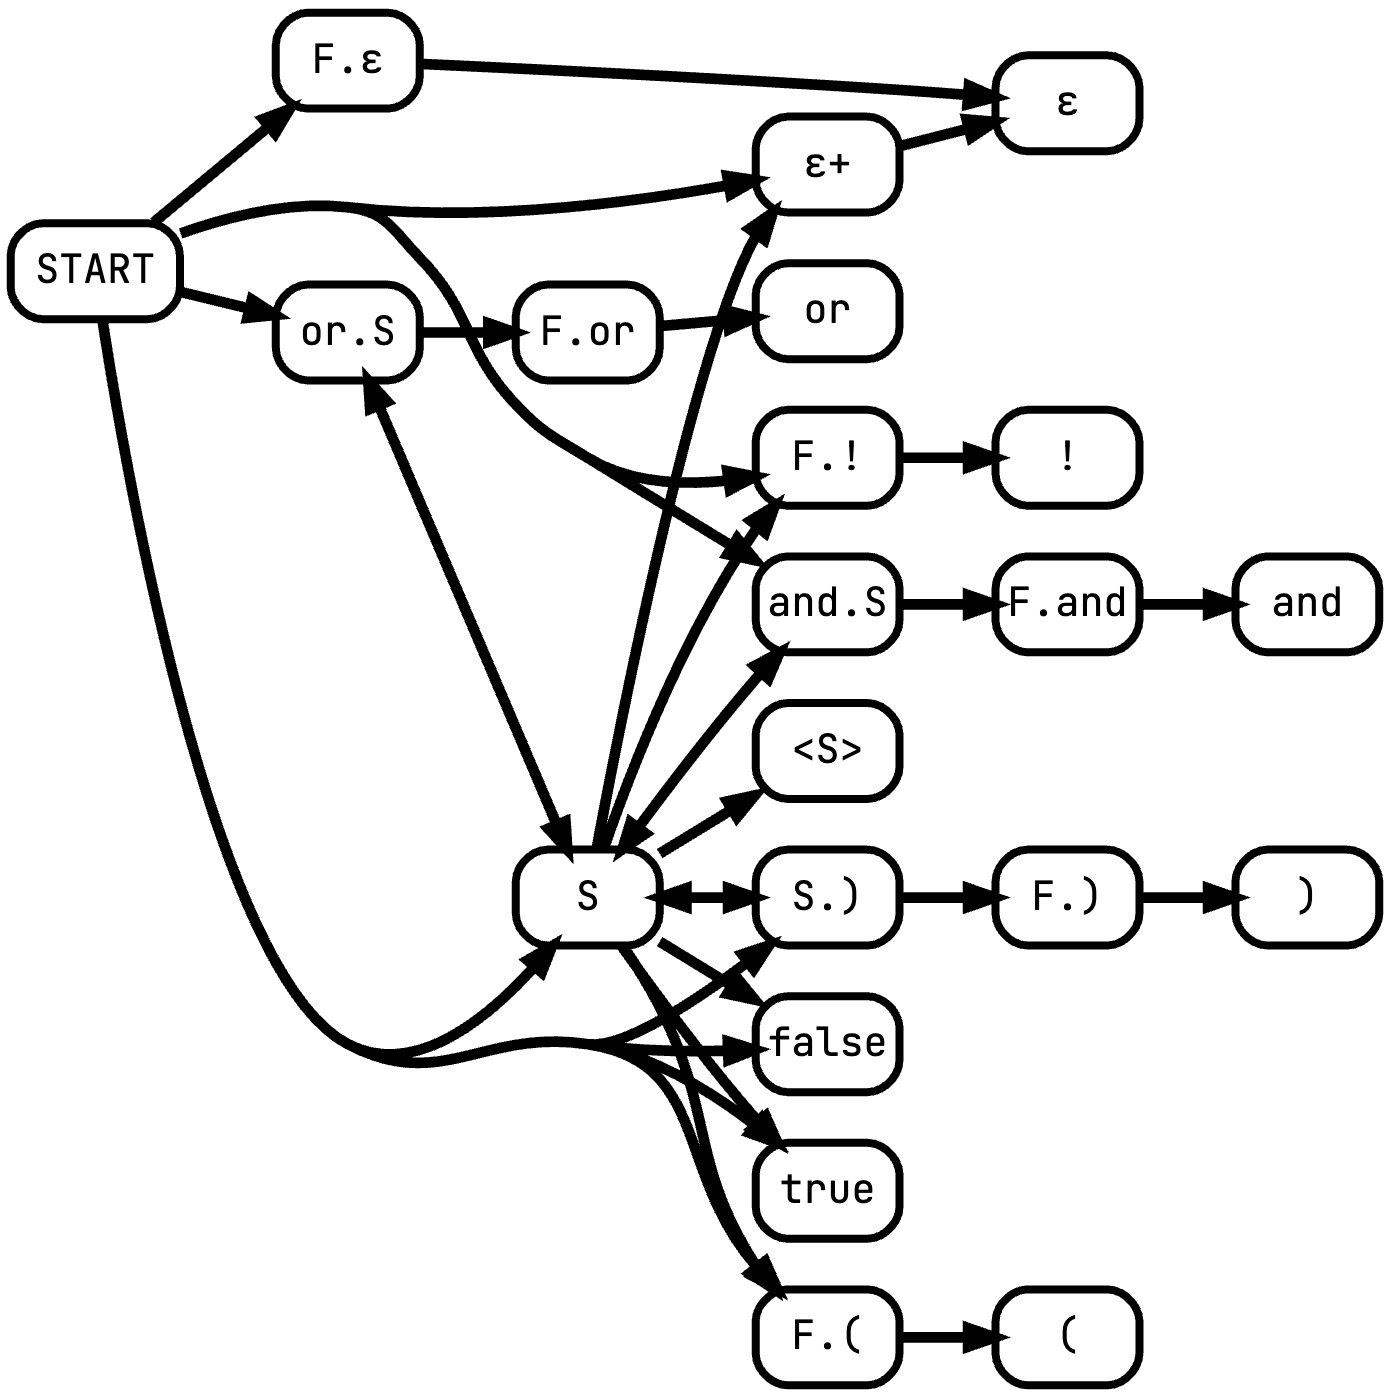
\includegraphics[width=3.5cm]{../figures/bool_arith_cfg_graph.png}
%    \hspace{20pt}
%    \includegraphics[width=3.5cm]{../figures/bool_arith_cfg_mat.bmp}
%\end{figure}

\noindent Given a string containing holes such as the one below, Tidyparse will return several completions in a few milliseconds:

\begin{tcolorbox}
  \begin{lstlisting}[language=tidy, basicstyle=\ttfamily\small, escapeinside={(*@}{@*)}]
true _ _ _ ( false _ ( _ _ _ _ ! _ _ ) _ _ _ _(*@\caret{ }@*)
  \end{lstlisting}
  \tcblower
  \begin{lstlisting}[language=tidy, basicstyle=\ttfamily\small, escapeinside={(*@}{@*)}]
true (*@\hlorange{xor}@*) (*@\hlorange{!}@*) ( false (*@\hlorange{xor}@*) ( <S> (*@\hlorange{)}@*) or ! (*@\hlorange{<S>}@*) ) (*@\hlorange{xor}@*) (*@\hlorange{<S>}@*)
true (*@\hlorange{xor}@*) (*@\hlorange{!}@*) ( false (*@\hlorange{and}@*) ( <S> (*@\hlorange{)}@*) or ! (*@\hlorange{<S>}@*) ) (*@\hlorange{xor}@*) (*@\hlorange{<S>}@*)
true (*@\hlorange{xor}@*) (*@\hlorange{!}@*) ( false (*@\hlorange{and}@*) ( <S> (*@\hlorange{)}@*) and ! (*@\hlorange{<S>}@*) ) (*@\hlorange{xor}@*) (*@\hlorange{<S>}@*)
true (*@\hlorange{xor}@*) (*@\hlorange{!}@*) ( false (*@\hlorange{and}@*) ( <S> (*@\hlorange{)}@*) and ! (*@\hlorange{<S>}@*) ) (*@\hlorange{and}@*) (*@\hlorange{<S>}@*)
...
  \end{lstlisting}
\end{tcolorbox}

\noindent Similarly, if provided with a string containing various errors, Tidyparse will return several suggestions how to fix it, where \hlgreen{green} is insertion, \hlorange{orange} is substitution and \hlred{red} is deletion.


\begin{tcolorbox}
\begin{lstlisting}[language=tidy, basicstyle=\ttfamily\small, escapeinside={(*@}{@*)}]
true and ( false or and true false(*@\caret{ }@*)
\end{lstlisting}
\tcblower
\begin{lstlisting}[language=tidy, basicstyle=\ttfamily\small, escapeinside={(*@}{@*)}]
1.) true and ( false or (*@\hlorange{!}@*) true (*@\hlorange{)}@*)
2.) true and ( false or (*@\hlgreen{<S>}@*) and true (*@\hlorange{)}@*)
3.) true and ( false or (*@\hlorange{(}@*) true (*@\hlorange{)}@*) (*@\hlgreen{)}@*)
...
9.) true and ( false or (*@\hlgreen{!}@*) (*@\hlgreen{<S>}@*) (*@\hlgreen{)}@*) and true (*@\hlred{false} @*)
\end{lstlisting}
\end{tcolorbox}

\noindent In the following paper, we will describe how we built it.

\section{Matrix Theory}\label{sec:matrix}

Recall that a CFG is a quadruple consisting of terminals $(\Sigma)$, nonterminals $(V)$, productions $(P\colon V \rightarrow (V \mid \Sigma)^*)$, and a start symbol, $(S)$. It is a well-known fact that every CFG is reducible to \textit{Chomsky Normal Form}, $P'\colon V \rightarrow (V^2 \mid \Sigma)$, in which every production takes one of two forms, either $w \rightarrow xz$, or $w \rightarrow t$, where $w, x, z: V$ and $t: \Sigma$. For example, the CFG, $P:=\{S \rightarrow S S \mid ( S ) \mid ()\}$, corresponds to the CNF:\vspace{-3pt}

\begin{table}[H]
\begin{tabular}{llll}
$P'=\big\{\;S\rightarrow QR \mid SS \mid LR,$ & $L \rightarrow (,$ & $R \rightarrow ),$ & $Q\rightarrow LS\;\big\}$
\end{tabular}
\end{table}\vspace{-8pt}

\noindent Given a CFG, $\mathcal{G}' : \langle \Sigma, V, P, S\rangle$ in CNF, we can construct a recognizer $R: \mathcal{G}' \rightarrow \Sigma^n \rightarrow \mathbb{B}$ for strings $\sigma: \Sigma^n$ as follows. Let $2^V$ be our domain, $0$ be $\varnothing$, $\oplus$ be $\cup$, and $\otimes$ be defined as:\vspace{-10pt}

\begin{align}
X \otimes Z := \big\{\;w \mid \langle x, z\rangle \in X \times Z, (w\rightarrow xz) \in P\;\big\}
\end{align}

\noindent If we define $\sigma_r^{\shur} \coloneqq \{w \mid (w \rightarrow \sigma_r) \in P\}$, then initialize $M^0_{r+1=c}(\mathcal{G}', e) := \;\sigma_r^{\shur}$ and solve for the fixpoint $M^* = M + M^2$,\vspace{-10pt}

\begin{align*}
  M^0:=\begin{pNiceMatrix}[nullify-dots,xdots/line-style=loosely dotted]
         \varnothing & \sigma_1^\shri & \varnothing & \Cdots & \varnothing \\
         \Vdots      & \Ddots         & \Ddots      & \Ddots & \Vdots\\
                     &                &             &        & \varnothing\\
                     &                &             &        & \sigma_n^\shup \\
         \varnothing & \Cdots         &             &        & \varnothing
  \end{pNiceMatrix} &\Rightarrow M^* =
  \begin{pNiceMatrix}[nullify-dots,xdots/line-style=loosely dotted]
    \varnothing & \sigma_1^\shri & \Lambda & \Cdots & \Lambda^*_\sigma\\
    \Vdots      & \Ddots         & \Ddots  & \Ddots & \Vdots\\
                &                &         &        & \Lambda\\
                &                &         &        & \sigma_n^\shup \\
    \varnothing & \Cdots         &         &        & \varnothing
  \end{pNiceMatrix}
\end{align*}

\noindent we obtain the recognizer, $R(\mathcal{G}', \sigma) := S \in \Lambda^*_\sigma? \Leftrightarrow \sigma \in \mathcal{L}(\mathcal{G})?$

This decision procedure can be abstracted by lifting into the domain of bitvector variables, producing an algebraic expression for each scalar inhabitant of the northeasternmost bitvector $\mathcal{T}$, whose solutions correspond to valid parse forests for an incomplete string on the superdiagonal. Note that $\bigoplus_{c = 1}^n M_{r,c} \otimes M_{c,r}$ has cardinality bounded by $|V|$ and is thus representable as a fixed-length vector using the characteristic function, $\mathds{1}$. In particular, $\oplus, \otimes$ are redefined as $\boxplus, \boxtimes$ over bitvectors so the following diagram commutes,\footnote{Hereinafter, we use gray highlighting to distinguish between expressions containing only \highlight{\text{constants}} from those which may contain free variables.}

\begin{figure}[H]
  \adjustbox{scale=0.82,center}{%
    \[\begin{tikzcd}[row sep=large, column sep=huge]
        \langle\mathcal{G}', \highlight{\Sigma}^{n-1}\rangle \arrow[leftrightarrow, drrr, shorten=-1mm] & & [-135pt] & \vspace{20pt}\text{Set} \arrow[d, phantom] & \text{Bit} \arrow[d, phantom] & [-90pt] & \langle\mathcal{G}', \Sigma^{n-1}\rangle \arrow[drr, shorten=-2mm] & [-90pt] & \text{SAT} \arrow[d, phantom]\\[-30pt]
        \text{Rubix}  \arrow[rr, phantom] & & [-135pt] & M \times M \arrow[r, "\mathds{1}^{2^{n\times n}}", labels=above] \arrow[d, "\hspace{-13pt}\bigoplus\:\bigotimes"] & \mathbb{Z}_2^{|V|^{n\times n}} \times \mathbb{Z}_2^{|V|^{n\times n}} \arrow[d, "\hspace{-13.4pt}\highlight{+}\:\highlight{*}"] \arrow[l, "\mathds{1}^{-2^{n\times n}}", labels=below] \arrow[rrrr, rightarrowtail, "\varphi^{2^{n\times n}}", labels=above] & [-90pt] & & [-90pt] & \mathcal{M} \times \mathcal{M} \arrow[llll, rightharpoonup, shorten=1mm, "\varphi^{-2^{n\times n}}", labels=below] \arrow[d, "\hspace{-9pt}+\:\:\:*"] \\
        \text{Matrix} \arrow[rr, phantom] & & [-135pt] & 2^V \times 2^V \arrow[r, "\mathds{1}^{2}", labels=above] \arrow[d, "\hspace{-9pt}\oplus\:\otimes"] & \mathbb{Z}_2^{|V|} \times \mathbb{Z}_2^{|V|} \arrow[d, "\hspace{-15.8pt}\highlight{\boxplus}\:\highlight{\boxtimes}"] \arrow[l, "\mathds{1}^{-2}", labels=below] \arrow[rrrr, rightarrowtail, "\varphi^2", labels=above] & [-90pt] & & [-90pt] & \mathcal{V} \times \mathcal{V} \arrow[llll, rightharpoonup, shorten=1mm, "\varphi^{-2}", labels=below] \arrow[d, "\hspace{-9.5pt}\boxplus\:\boxtimes"] \arrow[u] \\
        \text{Vector} \arrow[rr, phantom] & & [-135pt] & 2^V \arrow[r, "\mathds{1}", labels=above] & \mathbb{Z}_2^{|V|} \arrow[l, "\mathds{1}^{-1}", labels=below] \arrow[rrrr, rightarrowtail, "\varphi", labels=above] & [-90pt] & & [-90pt] & \mathcal{V} \arrow[llll, rightharpoonup, shorten=1mm, "\varphi^{-1}", labels=below] \arrow[u]
    \end{tikzcd}\]
  }
\end{figure}

\noindent where $\mathcal{V}$ is a function $\mathbb{Z}_2^{|V|}\rightarrow\mathbb{Z}_2$. Note that while always possible to encode $\mathbb{Z}_2^{|V|} \rightarrow \mathcal{V}$ using the identity function, $\varphi^{-1}$ may not exist, as an arbitrary $\mathcal{V}$ might have zero, one, or in general, multiple solutions in $\mathbb{Z}_2^{|V|}$.

\noindent Full details of the bisimilarity between parsing and matrix multiplication can be found in Valiant~\cite{valiant1975general}, who shows its time complexity to be $\mathcal{O}(n^\omega)$ where $\omega$ is the matrix multiplication bound ($\omega < 2.77$), and Lee~\cite{lee2002fast}, who shows that speedups to Boolean matrix multiplication are realizable by CFL parsers. Assuming sparsity, this technique is typically linearithmic, and is believed to be the most efficient general procedure for CFL recognition.

%\noindent The compactness of this representation can be improved via a combinatorial number system without loss of generality, although $\mathds{1}$ is a convenient encoding for SAT.


\subsection{Encoding CFG parsing as SAT solving}\label{sec:sat}

%We precompute the shadow of fully-resolved substrings before feeding it to the SAT solver. If the substring is known, we can simply compute this directly outside the SAT solver. Shaded regions are bitvector literals and light regions correspond to bitvector variables.

%We illustrate this fact in \S\ref{sec:error}:
%
%\begin{figure}[H]
%    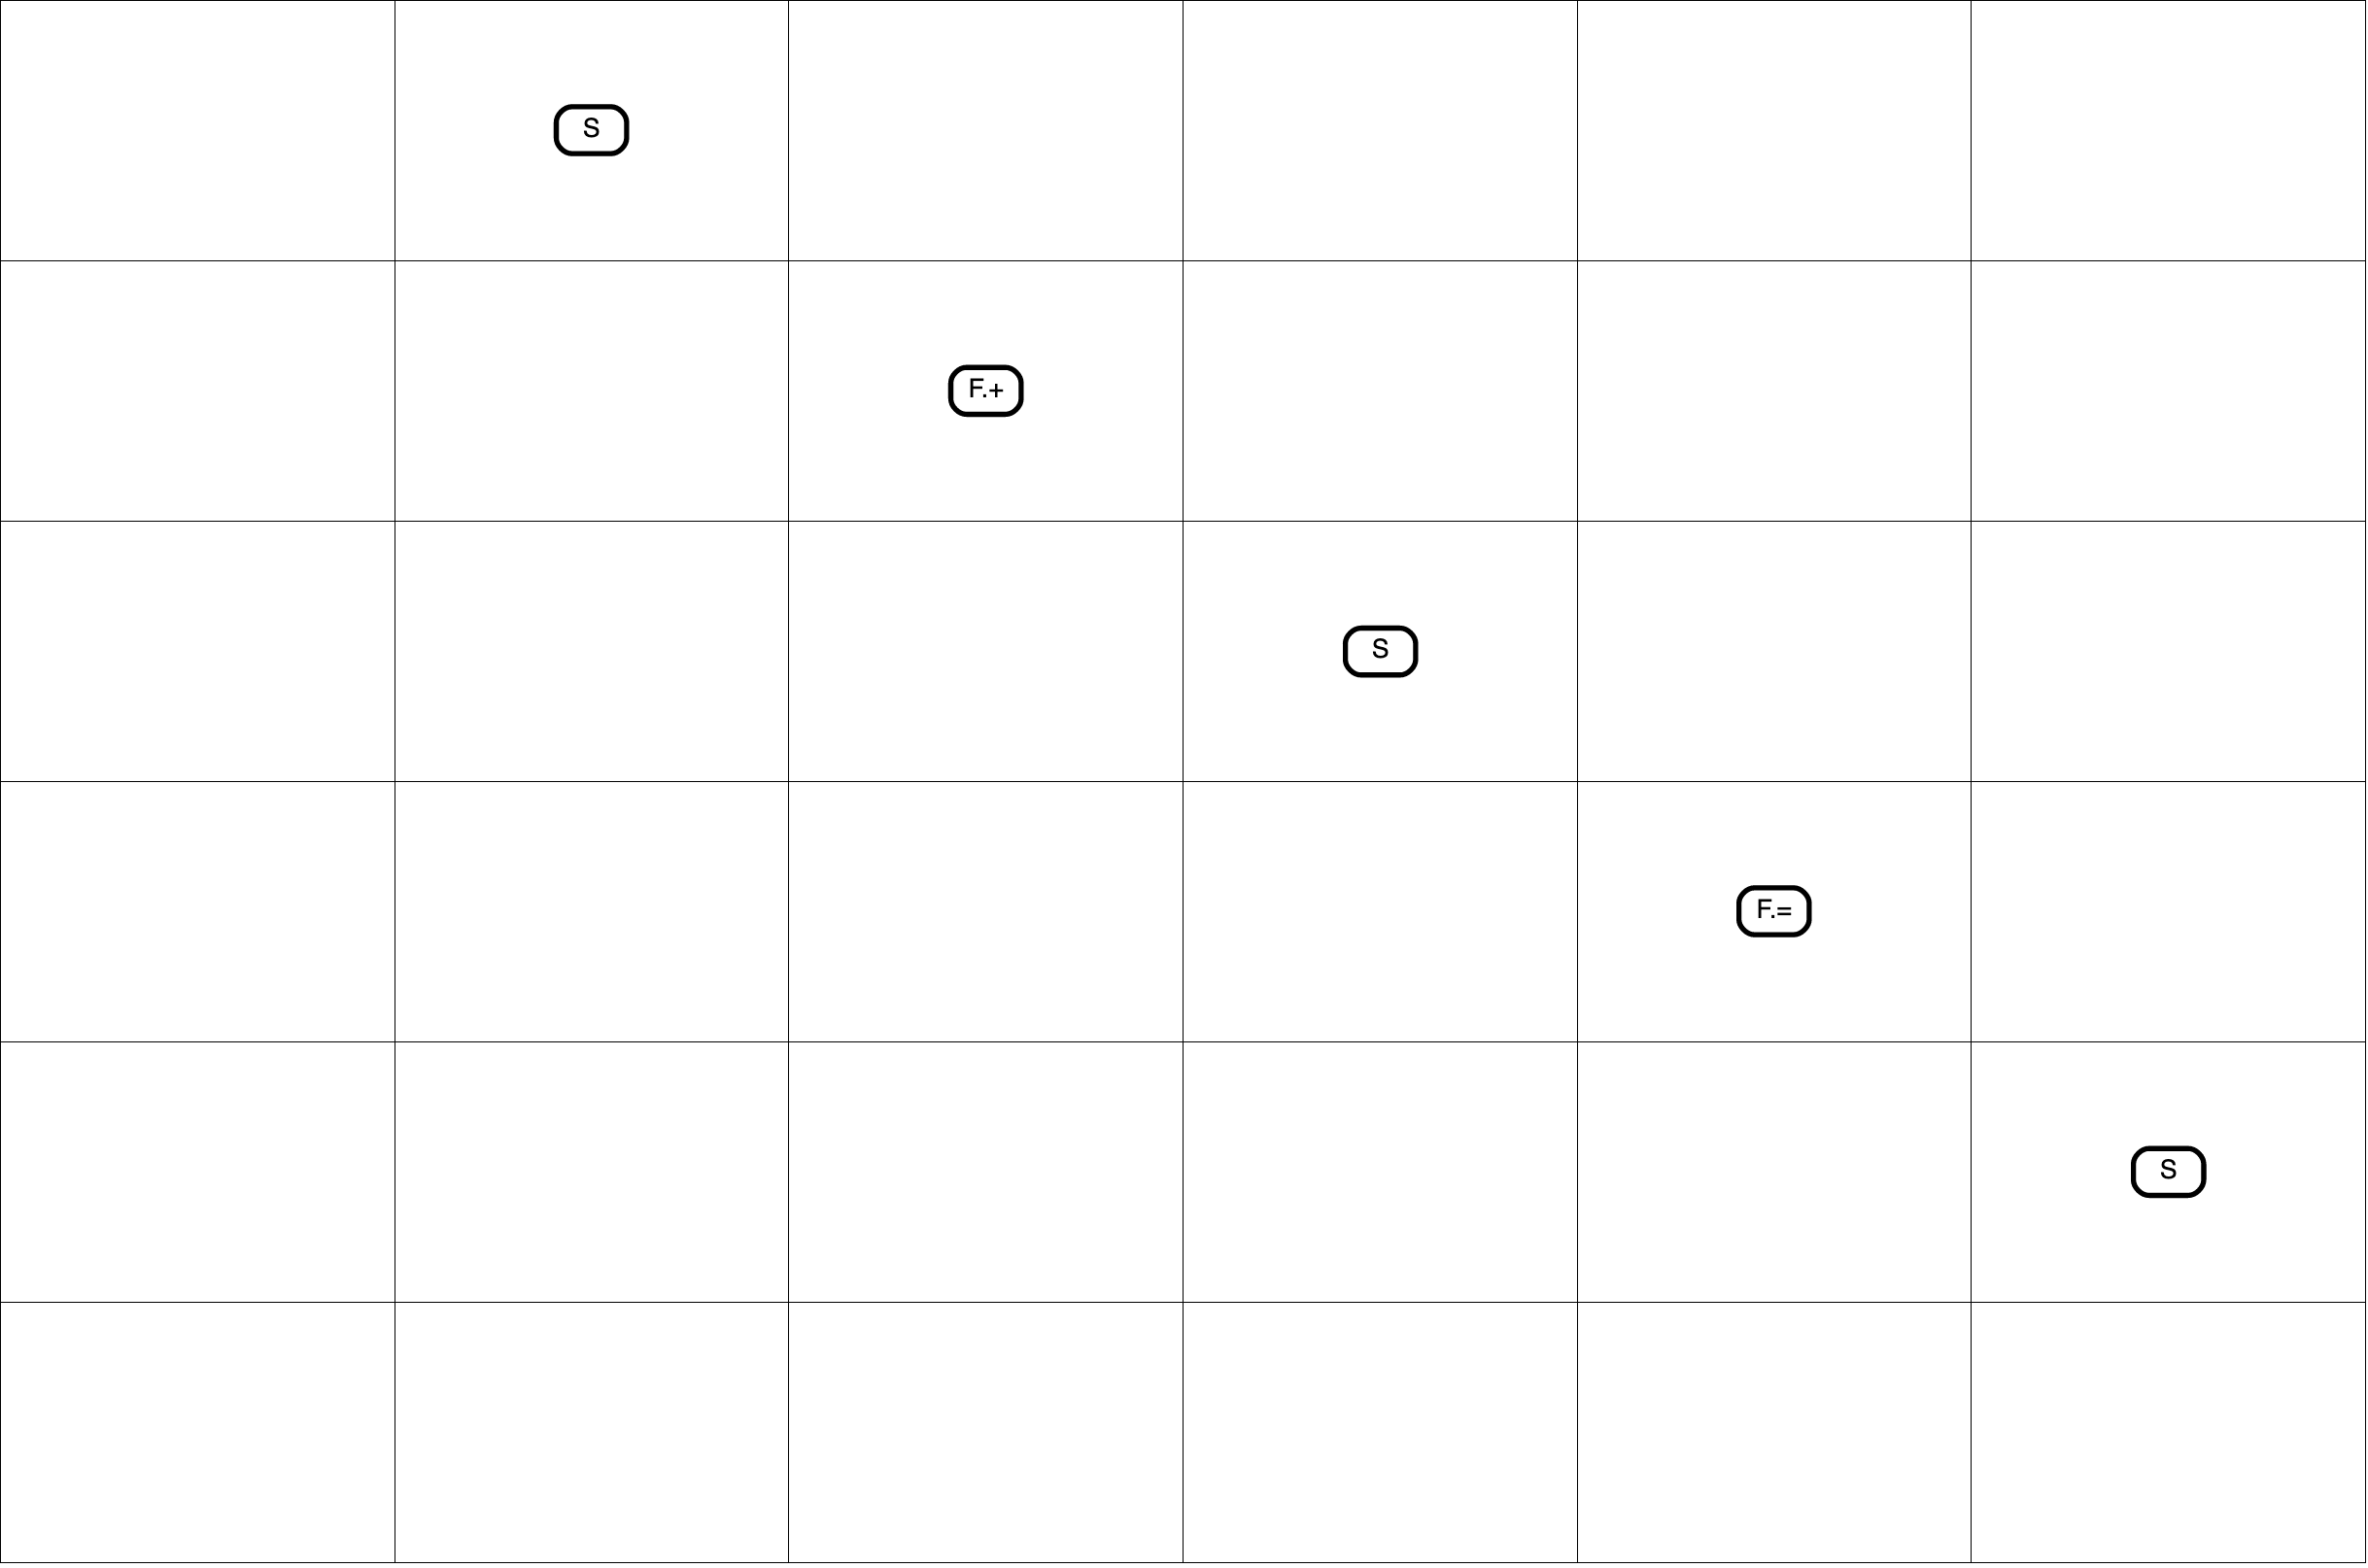
\includegraphics[width=2cm]{../figures/parse1.png}
%    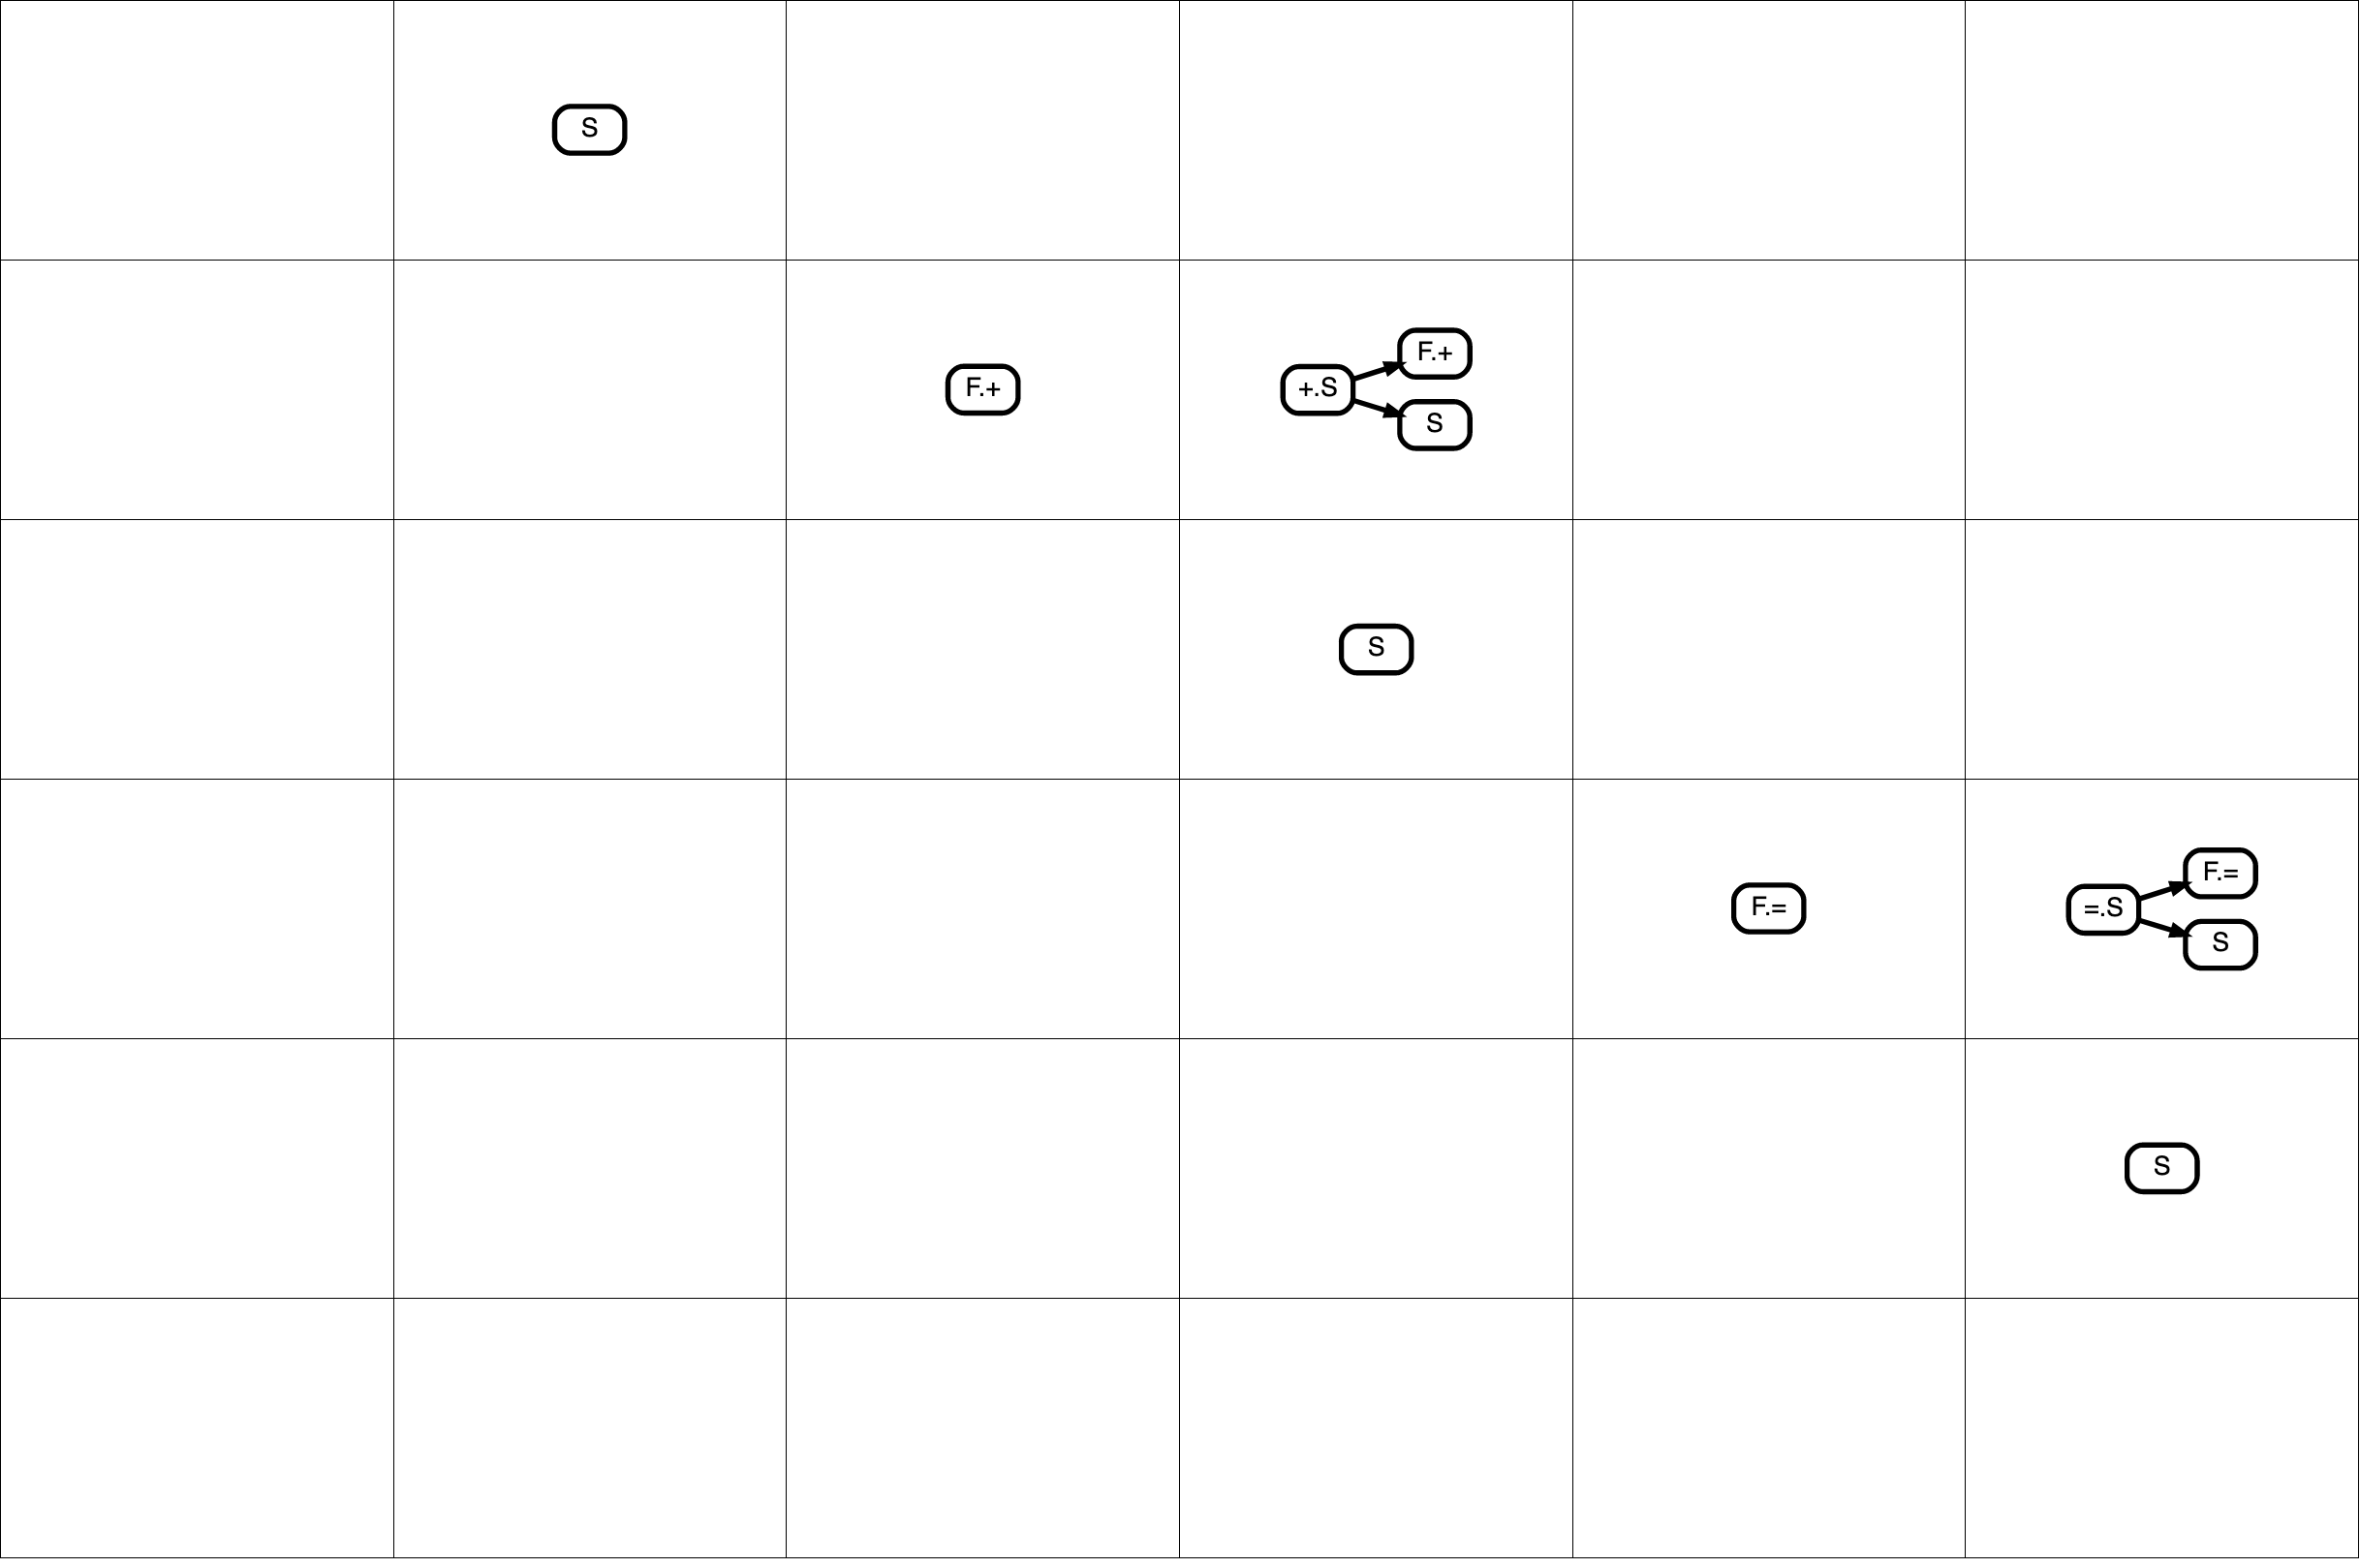
\includegraphics[width=2cm]{../figures/parse2.png}
%    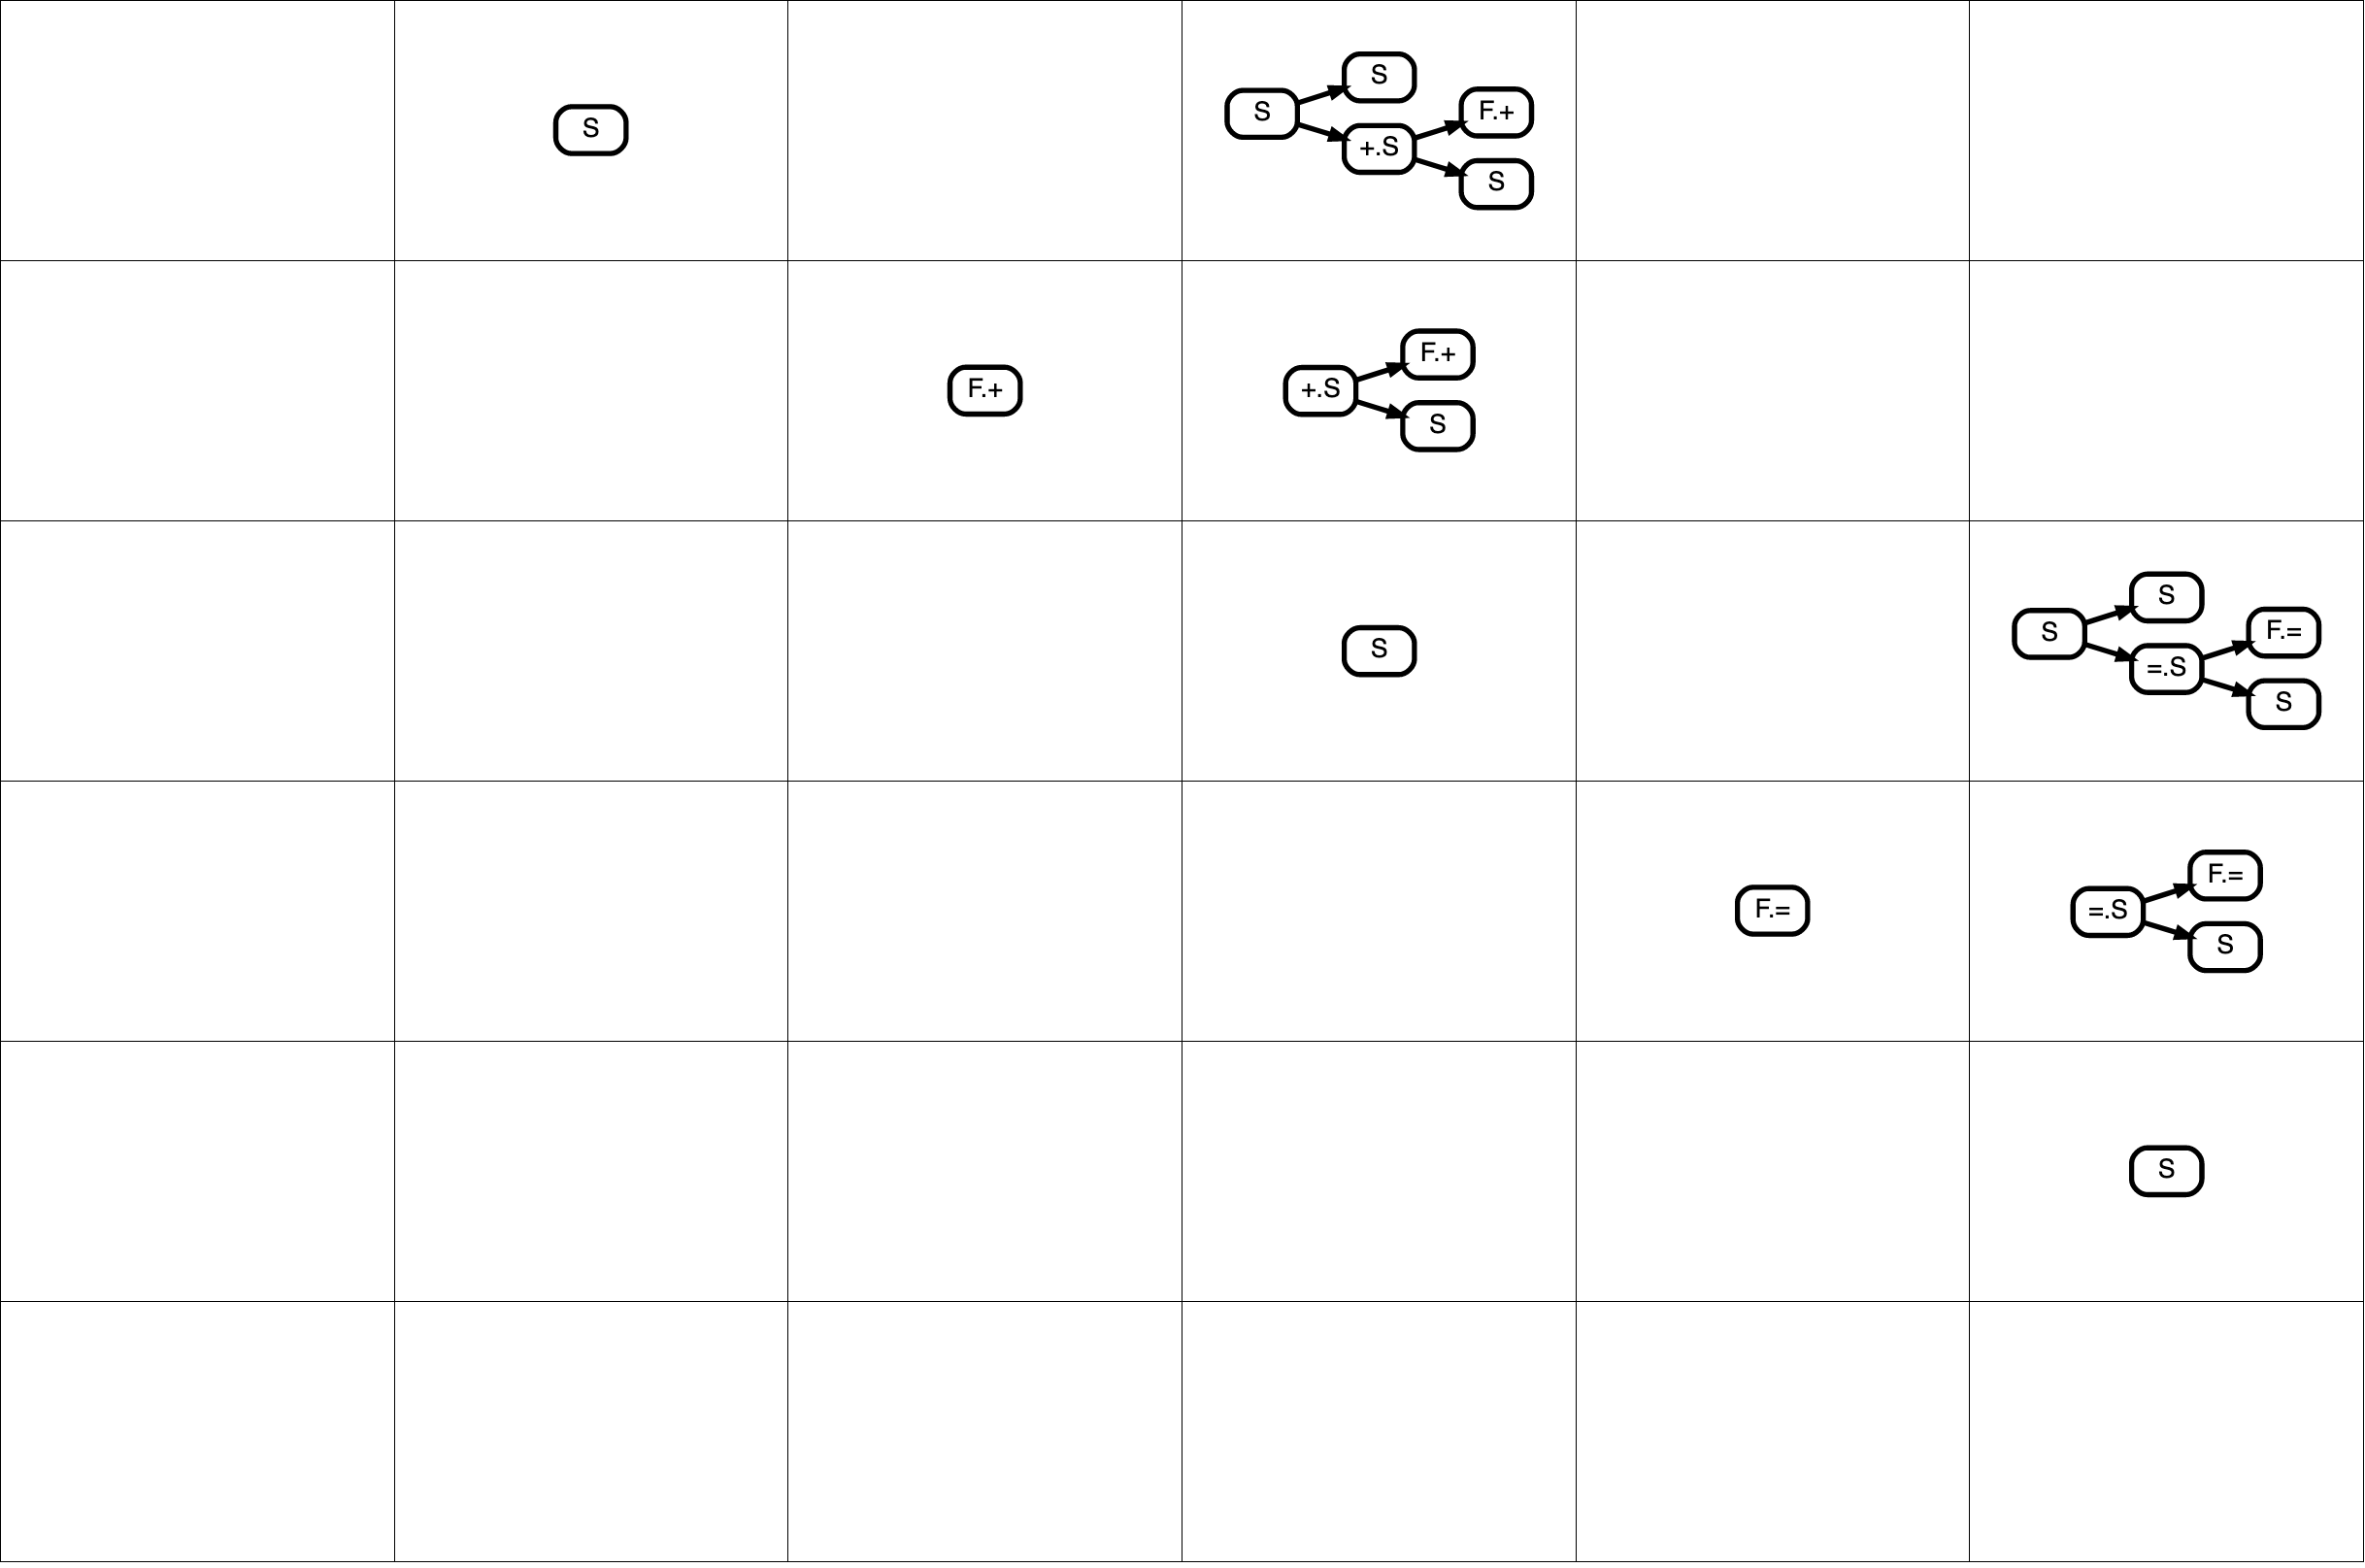
\includegraphics[width=2cm]{../figures/parse3.png}
%    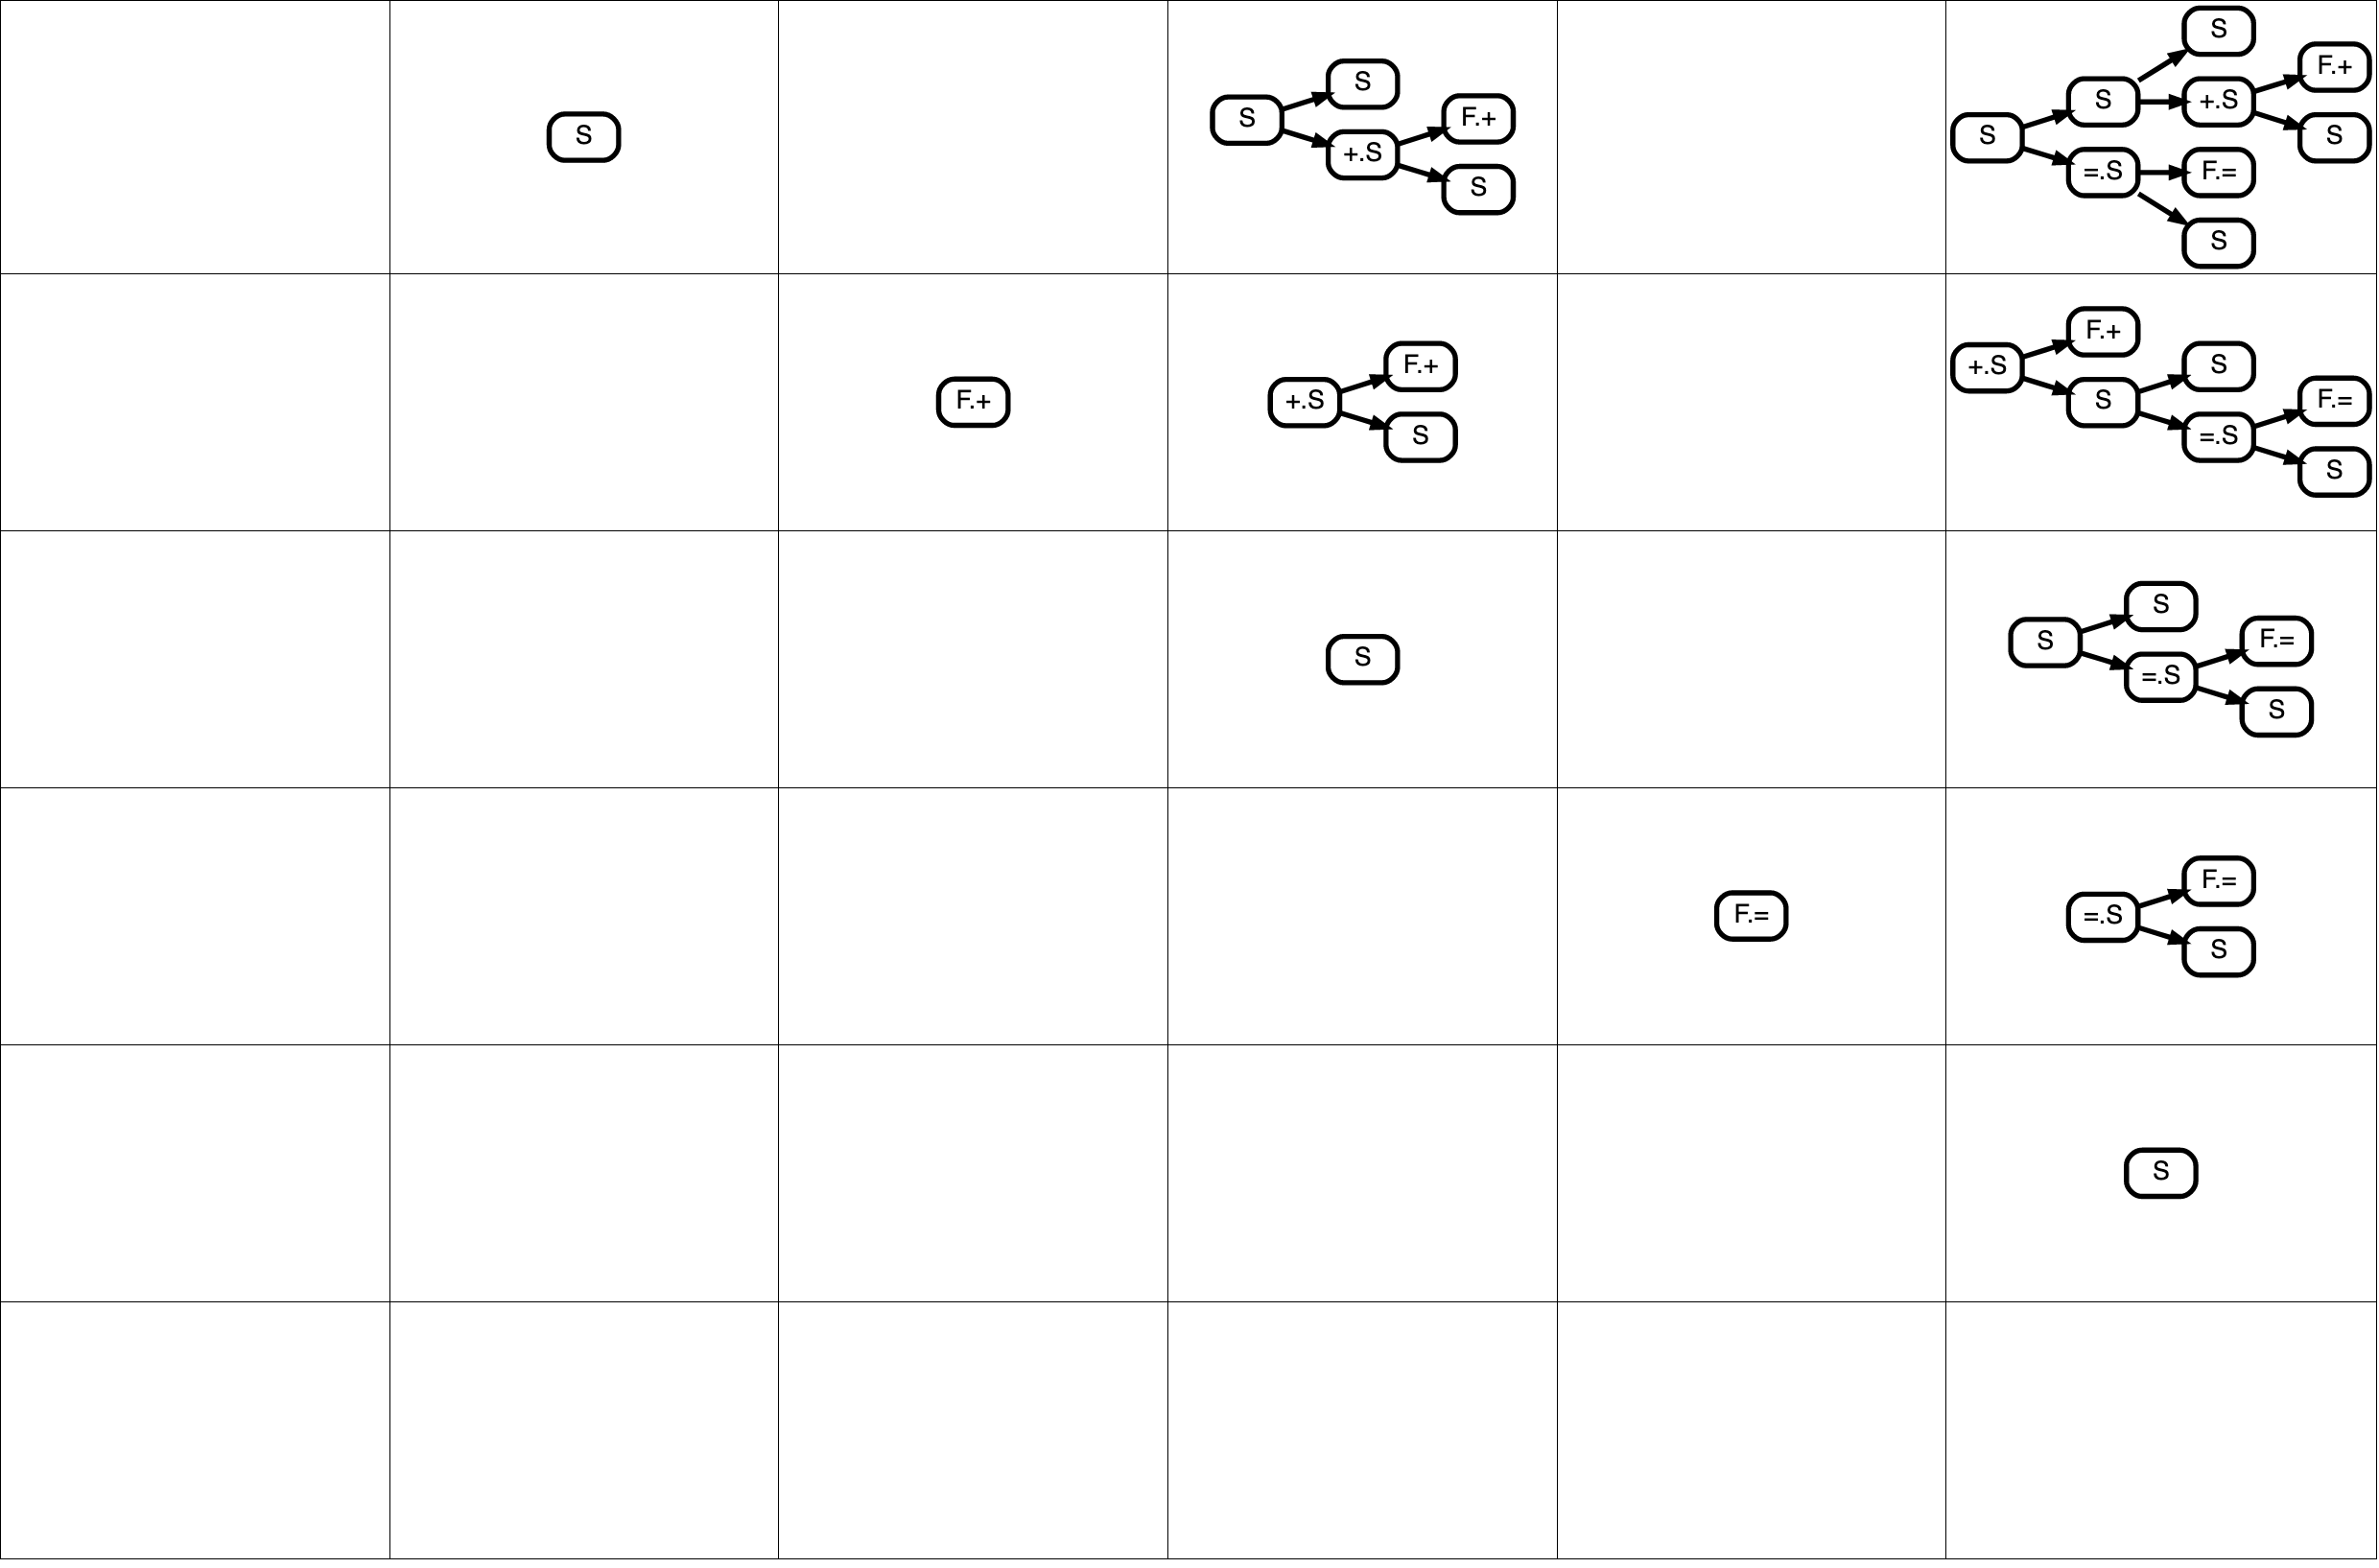
\includegraphics[width=2cm]{../figures/parse4.png}
%\end{figure}

\newcommand\ddd{\Ddots}
\newcommand\vdd{\Vdots}
\newcommand\cdd{\Cdots}
\newcommand\lds{\ldots}
\newcommand\vno{\varnothing}
\newcommand{\ts}[1]{\textsuperscript{#1}}
\newcommand\non{1\ts{st}}
\newcommand\ntw{2\ts{nd}}
\newcommand\nth{3\ts{rd}}
\newcommand\nfo{4\ts{th}}
\newcommand\nfi{5\ts{th}}
\newcommand\nsi{6\ts{th}}
\newcommand\nse{7\ts{th}}
\newcommand{\vs}[1]{\sigma_{#1}^{\shur}}
\newcommand\rcr{\rowcolor{black!15}}
\newcommand\rcw{\rowcolor{white}}
\newcommand\pcd{\cdot}
\newcommand\pcp{\phantom\cdot}
\newcommand\ppp{\phantom{\nse}}

\begin{figure}[H]
    \[
        \mathbf{M}^* = \begin{pNiceArray}{>{\strut}ccccccc}[margin, extra-margin=2pt,colortbl-like, xdots/line-style=loosely dotted]
            \vno & \rcr \vs{1} &  \mathcal{L}_{1,3} & \mathcal{L}_{1,3} & \rcw \mathcal{V}_{1,4} & \cdd & \mathcal{V}_{1,n} \\
            \vdd & \ddd        &  \rcr\vs{2}        & \mathcal{L}_{2,3} & \rcw\vdd               &      & \vdd \\
                 &             &                    & \rcr\vs{3}        & \rcw                   &      & \\
                 &             &                    &                   & \mathcal{V}_{4,4}      &      & \\
                 &             &                    &                   &                        & \ddd & \\
                 &             &                    &                   &                        &      & \mathcal{V}_{n,n} \\
            \vno & \cdd        &                    &                   &                        &      & \vno
        \end{pNiceArray}
    \]
\end{figure}

\noindent Depicted above is a SAT tensor representing \hlgray{$\sigma_1\:\sigma_2\:\sigma_3$}$\:\_\:\ldots\:\_$ where shaded regions demarcate known bitvector literals $\mathcal{L}_{r,c}$ (i.e., representing established nonterminal forests) and unshaded regions correspond to bitvector variables $\mathcal{V}_{r,c}$ (i.e., representing seeded nonterminal forests to be grown). Since $\mathcal{L}_{r,c}$ are fixed, we precompute them outside the SAT solver.

\section{Error Recovery}\label{sec:error}

Unlike classical parsers which need special care to recover from errors, if the input string does not parse, Tidyparse can return partial subtrees. If no solution exists, the upper triangular entries will appear as a jagged-shaped ridge whose peaks represent the roots of parsable ASTs. These provide a natural debugging environment to aid the repair process.

The matrix $\mathcal{M}^*$ encodes a superposition of all labeled binary trees of a fixed breadth. Consider the string \texttt{\_ ... \_}, which might generate various parse trees, with labels omitted to emphasize their structure:

\begin{figure}[H]
  \resizebox{0.99\textwidth}{!}{
    \[
      \mathbf{M}^* = \begin{pNiceArray}{>{\strut}ccccccc}[margin, extra-margin=2pt,colortbl-like, xdots/line-style=loosely dotted]
         \tikzmark{a} & \tikzmark{k}  & \tikzmark{b} & \tikzmark{m} & \tikzmark{c} & \tikzmark{q} & \tikzmark{d} \\
                 \vno & \tikzmark{l}  &              & \tikzmark{n} &              & \tikzmark{r} & \tikzmark{w} \\
                 \vdd & \ddd          & \tikzmark{e} & \tikzmark{o} & \tikzmark{f} & \tikzmark{s} & \tikzmark{g} \\
                      &               &              & \tikzmark{p} &              & \tikzmark{t} & \tikzmark{x} \\
                      &               &              &              & \tikzmark{h} & \tikzmark{u} & \tikzmark{i} \\
                      &               &              &              &              & \tikzmark{v} &              \\
                 \vno & \cdd          &              &              &              & \vno         & \tikzmark{j}
      \end{pNiceArray}
      \begin{tikzpicture}[overlay, remember picture, blubr/.style={-,blue}, redbr/.style={-,red}, grnbr/.style={-,green}]
        \draw [grnbr] ({pic cs:l}) to ({pic cs:r});
        \draw [grnbr] ({pic cs:v}) to ({pic cs:r});
        \draw [grnbr] ({pic cs:r}) to ({pic cs:w});
        \draw [blubr] ({pic cs:a}) to ({pic cs:b});
        \draw [blubr] ({pic cs:e}) to ({pic cs:b});
        \draw [blubr] ({pic cs:h}) to ({pic cs:c});
        \draw [blubr] ({pic cs:b}) to ({pic cs:c});
        \draw [blubr] ({pic cs:c}) to ({pic cs:d});
        \draw [redbr] ({pic cs:h}) to ({pic cs:i});
        \draw [redbr] ({pic cs:j}) to ({pic cs:i});
        \draw [redbr] ({pic cs:e}) to ({pic cs:g});
        \draw [redbr] ({pic cs:i}) to ({pic cs:g});
        \draw [redbr] ({pic cs:g}) to ({pic cs:d});
      \end{tikzpicture}\Rightarrow
      \left\{\begin{pNiceArray}{>{\strut}ccccccc}[margin, extra-margin=2pt,colortbl-like, xdots/line-style=loosely dotted]
        \tikzmark{a1} & \tikzmark{k1}  & \tikzmark{b1} & \tikzmark{m1} & \tikzmark{c1} & \tikzmark{q1} & \tikzmark{d1} \\
        \vno          & \tikzmark{l1}  &               & \tikzmark{n1} &               & \tikzmark{r1} & \tikzmark{w1} \\
        \vdd          & \ddd           & \tikzmark{e1} & \tikzmark{o1} & \tikzmark{f1} & \tikzmark{s1} & \tikzmark{g1} \\
                      &                &               & \tikzmark{p1} &               & \tikzmark{t1} & \tikzmark{x1} \\
                      &                &               &               & \tikzmark{h1} & \tikzmark{u1} & \tikzmark{i1} \\
                      &                &               &               &               & \tikzmark{v1} &              \\
        \vno          & \cdd           &               &               &               & \vno          & \tikzmark{j1}
      \end{pNiceArray}
      \begin{tikzpicture}[overlay, remember picture, redbr/.style={-,red}]
        \draw [redbr] ({pic cs:a1}) to ({pic cs:d1});
        \draw [redbr] ({pic cs:h1}) to ({pic cs:i1});
        \draw [redbr] ({pic cs:j1}) to ({pic cs:i1});
        \draw [redbr] ({pic cs:e1}) to ({pic cs:g1});
        \draw [redbr] ({pic cs:i1}) to ({pic cs:g1});
        \draw [redbr] ({pic cs:g1}) to ({pic cs:d1});
      \end{tikzpicture}_{\textstyle,}
      \begin{pNiceArray}{>{\strut}ccccccc}[margin, extra-margin=2pt,colortbl-like, xdots/line-style=loosely dotted]
        \tikzmark{a2} & \tikzmark{k2}  & \tikzmark{b2} & \tikzmark{m2} & \tikzmark{c2} & \tikzmark{q2} & \tikzmark{d2} \\
        \vno          & \tikzmark{l2}  &               & \tikzmark{n2} &               & \tikzmark{r2} & \tikzmark{w2} \\
        \vdd          & \ddd           & \tikzmark{e2} & \tikzmark{o2} & \tikzmark{f2} & \tikzmark{s2} & \tikzmark{g2} \\
                      &                &               & \tikzmark{p2} &               & \tikzmark{t2} & \tikzmark{x2} \\
                      &                &               &               & \tikzmark{h2} & \tikzmark{u2} & \tikzmark{i2} \\
                      &                &               &               &               & \tikzmark{v2} &              \\
        \vno          & \cdd           &               &               &               & \vno          & \tikzmark{j2}
      \end{pNiceArray}
      \begin{tikzpicture}[overlay, remember picture, blubr/.style={-,blue}]
        \draw [blubr] ({pic cs:a2}) to ({pic cs:b2});
        \draw [blubr] ({pic cs:e2}) to ({pic cs:b2});
        \draw [blubr] ({pic cs:h2}) to ({pic cs:c2});
        \draw [blubr] ({pic cs:b2}) to ({pic cs:c2});
        \draw [blubr] ({pic cs:c2}) to ({pic cs:d2});
        \draw [blubr] ({pic cs:j2}) to ({pic cs:d2});
      \end{tikzpicture}_{\textstyle,}
      \begin{pNiceArray}{>{\strut}ccccccc}[margin, extra-margin=2pt,colortbl-like, xdots/line-style=loosely dotted]
        \tikzmark{a3} & \tikzmark{k3}  & \tikzmark{b3} & \tikzmark{m3} & \tikzmark{c3} & \tikzmark{q3} & \tikzmark{d3} \\
        \vno          & \tikzmark{l3}  &               & \tikzmark{n3} &               & \tikzmark{r3} & \tikzmark{w3} \\
        \vdd          & \ddd           & \tikzmark{e3} & \tikzmark{o3} & \tikzmark{f3} & \tikzmark{s3} & \tikzmark{g3} \\
                      &                &               & \tikzmark{p3} &               & \tikzmark{t3} & \tikzmark{x3} \\
                      &                &               &               & \tikzmark{h3} & \tikzmark{u3} & \tikzmark{i3} \\
                      &                &               &               &               & \tikzmark{v3} &              \\
        \vno          & \cdd           &               &               &               & \vno          & \tikzmark{j3}
      \end{pNiceArray}
      \begin{tikzpicture}[overlay, remember picture, grnbr/.style={-,green}]
        \draw [grnbr] ({pic cs:l3}) to ({pic cs:r3});
        \draw [grnbr] ({pic cs:n3}) to ({pic cs:p3});
        \draw [grnbr] ({pic cs:v3}) to ({pic cs:r3});
        \draw [grnbr] ({pic cs:r3}) to ({pic cs:w3});
        \draw [grnbr] ({pic cs:j3}) to ({pic cs:d3});
        \draw [grnbr] ({pic cs:a3}) to ({pic cs:d3});
      \end{tikzpicture}\ldots\right\}
    \]
  }
\end{figure}

Occasionally, it is not possible to decode a full tree. In a typical parser, error recovery requires special tricks. Here, we simply analyze the structure of the matrix $\mathbf{M}$ to decode the parseable subtrees:

\begin{figure}[H]
  \hspace{-0.5cm}\begin{minipage}[l]{6cm}
      \[
        \begin{NiceMatrix}
          \leftarrow & \nse & \nsi & \nfi & \nfo & \nth & \ntw & \non & \leftarrow & \ppp \\
                     &      & \ddd & \ddd & \ddd & \ddd & \ddd & \ddd & \ddd & \ppp \\
      \sigma_1^\shri & \cdd &      & A    &      &      &      &      &      & \ppp \\
                \vno & \ddd &  T_A & \vdd &      &      &      &      &      & \ppp \\
                \vdd & \ddd &      & \pcd & \cdd &      & B    &      &      & \ppp \\
                     &      &      &      &      & T_B  & \vdd &      &      & \ppp \\
                     &      &      &      &      &      & \pcd & \cdd &      & C    \\
                     &      &      &      &      &      &      &      & T_C  & \vdd \\
                     &      &      &      &      &      &      & \xno &      & \\
                     &      &      &      &      &      &      &      &      & \\
                     &      &      &      &      &      &      &      &      & \\
                     &      &      &      &      &      &      &      & \ppp & \sigma_n^\shup \\
                \vno & \cdd &      &      &      &      &      &      & \vno &
        \end{NiceMatrix}
    \]
  \end{minipage}
  \hspace{1cm}
  \begin{minipage}[l]{6cm}
      \begin{halftidyinput}
      (*@\err{\texttt{⊤ and ⊤ ! and ⊥ xor ⊤ ! ⊤ and ⊥}}\caret{ }@*)
      \end{halftidyinput}

      \begin{verbatim}
    Recovered 3 parseable leaves:
      \end{verbatim}
      \noindent\hspace{0.64cm}\emoji{herb}\hspace{1.70cm}\emoji{herb}\hspace{1.98cm}\emoji{herb}\vspace{-5pt}
      \begin{verbatim}
    └── ! [3]   └── and [4]   └── or [6]
      \end{verbatim}

      \begin{verbatim}
    Recovered 2 parseable branches:
      \end{verbatim}
    \hspace{0.63cm}\emoji{herb}\hspace{2.48cm}\emoji{herb}\vspace{-5pt}
      \begin{verbatim}
    └── S [0..2]     └── S [8..11]
        ├── ⊤ [0]        ├── S [8..9]
        ├── and [1]      │   ├── ! [8]
        └── ⊤ [2]        │   └── ⊤ [9]
                         ├── and [10]
                         └── ⊥ [11]
      \end{verbatim}
    \end{minipage}
  \caption{Peaks along the UT matrix ridge correspond to maximally parseable substrings. By recursing over upper diagonals of decreasing elevation and discarding all subtrees that fall under the shadow of another's canopy, we can recover the partial subtrees. The example depicted above contains three such branches, rooted at nonterminals $C, B, A$.}\label{fig:peaks}
\end{figure}

\noindent These branches correspond to peaks on the upper triangular (UT) matrix ridge. As depicted in Fig.~\ref{fig:peaks}, we traverse the peaks by decreasing elevation to collect partial AST branches.

\section{Tree Denormalization}

% https://www.ling.upenn.edu/advice/latex/qtree/qtreenotes.pdf
% https://cpb-us-w2.wpmucdn.com/campuspress.yale.edu/dist/0/119/files/2014/12/sec-10.17-drawing-arrows-2ek9r2b.pdf

Our parser emits a binary forest consisting of parse trees for the candidate string according to the CNF grammar, however this forest contains many so-called \textit{Krummholz}, or \textit{flag trees}, often found clinging to windy ridges and mountainsides.

\begin{figure}[H]
  \begin{minipage}{.45\linewidth}
    \begin{algorithm}[H]
      \caption{Tree denormalization}\label{alg:cap}
      \begin{algorithmic}
        \Procedure{Cut}{\texttt{t: Tree}}
          \State $\texttt{stems} \leftarrow \{\:\textsc{Cut}(\texttt{c}) \mid \texttt{c} \in \texttt{t.children}\:\}$
          \If{$\texttt{t.root} \in (V_{\mathcal{G}'} \setminus V_{\mathcal{G}})$}
            \State \textbf{return } \texttt{stems} %\Comment{Drop synthetic nonterminals.}
          \Else%\Comment{Graft the denormalized children on root.}
            \State \textbf{return } $\{\:\texttt{Tree(root, stems)}\:\}$
          \EndIf
        \EndProcedure
      \end{algorithmic}
    \end{algorithm}
  \end{minipage}
  \resizebox{.54\textwidth}{!}{
    \begin{tabular}{ll}
        \Tree [.\texttt{S} \tikz\node(v1){\texttt{true}} [.$\ccancel{\texttt{and.S}}$ \tikz\node(v3){\texttt{and}} [.\texttt{S} \tikz\node(v5){\texttt{(}} [.$\ccancel{\texttt{S.)}}$ [.\texttt{S} \tikz\node(v9){\texttt{false}} [.$\ccancel{\texttt{or.S}}$ \tikz\node(v11){\texttt{xor}} [.\texttt{S} \texttt{!} \texttt{true} ] ] ] \tikz\node(v7){\texttt{)}} ] ] ] ]
%    \Tree [.S [.NP John ] [.VP [.\tikz\node(v1){V}; sleeps ] ] ]
        \hspace{-2cm}
        &
        \Tree [.\texttt{S} \tikz\node(v2){\texttt{true}} \tikz\node(v4){\texttt{and}} [.\texttt{S} \tikz\node(v6){\texttt{(}} [.\texttt{S} \tikz\node(v10){\texttt{false}} \tikz\node(v12){\texttt{xor}} [.\texttt{S} \texttt{!} \texttt{true} ] ] \tikz\node(v8){\texttt{)}} ] ]\\\\\\
%    \Tree [.\tikz\node(v2){V}; [.\tikz\node(v3){V}; ] [.Adv {a lot} ] ]
        \hspace{1cm}\Huge{Pre-Denormalization} & \hspace{2cm}\Huge{Post-Denormalization}
    \end{tabular}
    \begin{tikzpicture}[overlay]
%    \draw [red,dashed,-stealth] (v1) to[bend left] (v2);
        \draw [red,dashed,-stealth] (v3) to[bend left] (v4);
%    \draw [red,dashed,-stealth] (v5) to[bend left] (v6);
        \draw [red,dashed,-stealth] (v7) to[bend left] (v8);
%    \draw [red,dashed,-stealth] (v9) to[bend right] (v10);
        \draw [red,dashed,-stealth] (v11) to[bend right] (v12);
    \end{tikzpicture}
  }
  \caption{Since $\mathcal{G}'$ contains synthetic nodes, to recover a parse tree congruent with the original grammar $\mathcal{G}$, we prune all synthetic nodes and graft their stems onto the grandparent via a simple recursive procedure (Alg.~\ref{alg:cap}).}%, which is used to denormalize both complete and partial ASTs (cf. \S~\ref{sec:error}) alike.}
%    \caption{Result of applying Algorithm~\ref{alg:cap} to the tree obtained by parsing the string: \texttt{true and ( false or ! true )}.}
\end{figure}

\section{Backpropagation of error}

%    Although holes may occur anywhere, let us consider two cases in which $\Sigma^+$ is strictly left- or right-constrained, i.e., $\highlight{x}z, x\highlight{z}: \Sigma^{|x|+|z|}$.

Valiant's $\otimes$-operator, which yields the set of productions unifying known factors in a binary CFG, naturally implies the existence of a left- and right-quotient, which yield the set of nonterminals that may appear the right or left side of a known factor and its corresponding root. In other words, a known factor not only implicates subsequent expressions that can be derived from it, but also adjacent factors that may be composed with it to form a given derivation.

\begin{table}[H]
  \adjustbox{center}{%
  \begin{tabular}{ccccc}
    Valiant's $\otimes$-operator && Left Quotient && Right Quotient \\\\
    $x \otimes y := \big\{\;w \mid (w \rightarrow x z)\in P\;\big\}$ &&
    $\frac{\partial}{\partial \cev{x}} := \big\{\;z \mid (w \rightarrow x z)\in P\;\big\}$ &&
    $\frac{\partial}{\partial \vec{z}} := \big\{\;x \mid (w \rightarrow x z)\in P\;\big\}$ \\\\
    \begin{tabular}{|c|c|}
      \hline
      \cellcolor{black!15}\hspace{-0.5mm}$x$\hspace{-0.5mm} & \cellcolor{black!15}\hspace{-0.95mm}$w$\hspace{-0.95mm} \\ \hline
      \multicolumn{1}{c|}{~} & \hspace{-0.95mm}$z$\hspace{-0.95mm} \\
      \cline{2-2}
    \end{tabular} &&
    \begin{tabular}{|c|c|}
      \hline
      \cellcolor{black!15}\hspace{-0.5mm}$x$\hspace{-0.5mm} & \cellcolor{black!15}\hspace{-0.95mm}$w$\hspace{-0.95mm} \\ \hline
      \multicolumn{1}{c|}{~} & \hspace{-0.95mm}$z$\hspace{-0.95mm} \\
      \cline{2-2}
    \end{tabular} &&
    \begin{tabular}{|c|c|}
      \hline
      \hspace{-0.5mm}$x$\hspace{-0.5mm} & \cellcolor{black!15}\hspace{-0.95mm}$w$\hspace{-0.95mm} \\ \hline
      \multicolumn{1}{c|}{~} & \cellcolor{black!15}\hspace{-0.95mm}$z$\hspace{-0.95mm} \\
      \cline{2-2}
    \end{tabular}
  \end{tabular}
  }
\end{table}

\noindent The left quotient coincides with the derivative operator first proposed by Brzozowski~\cite{brzozowski1964derivatives} and Antimirov~\cite{antimirov1996partial} over regular languages, lifted into the context-free setting (our work). When the root and LHS are fixed, e.g., $\frac{\partial S}{\partial \cev{x}}: (\cev{V} \rightarrow S) \rightarrow \vec{\mathcal{V}}$ returns the set of admissible nonterminals to the RHS. One may also consider a gradient operator, $\cev{\nabla} S: (\cev{\mathcal{V}} \rightarrow S) \rightarrow \vec{\mathcal{V}}$, which simultaneously tracks the partials with respect to a set of multiple LHS nonterminals produced by a fixed root.

%  These operators in the context-free setting respect linearity. The $\oplus$ case is trivial. For $\otimes$, let us consider the left quotient. Its symmetric case is left as an exercise for the reader:
%
%  $\frac{\partial}{\partial x}(f\otimes g) = \frac{\partial f}{\partial x}\otimes g \oplus f\otimes\frac{\partial g}{\partial x}$
%
%  TODO: prove the product rule holds for CFG reachability.

If the root itself is unknown, we can define an operator, $\mathcal{H}_{\mathcal{W}\subseteq\mathcal{V}}: (\cev{\mathcal{V}}\times\vec{\mathcal{V}}\times\mathcal{W}) \rightarrow (\vec{\mathcal{V}}\times\vec{\mathcal{V}}\rightarrow\mathcal{W})$, which tracks second-order partial derivatives for all roots in $\mathcal{W}$. Unlike differential calculus on smooth manifolds, partials in this calculus do not necessarily commute depending on the CFG.

\definecolor{R}{RGB}{202,65,55}
\definecolor{G}{RGB}{151,216,56}
\definecolor{W}{RGB}{255,255,255}
\definecolor{X}{RGB}{65,65,65}

\newcommand{\TikZRubikFaceLeft}[9]{\def\myarrayL{#1,#2,#3,#4,#5,#6,#7,#8,#9}}
\newcommand{\TikZRubikFaceRight}[9]{\def\myarrayR{#1,#2,#3,#4,#5,#6,#7,#8,#9}}
\newcommand{\TikZRubikFaceTop}[9]{\def\myarrayT{#1,#2,#3,#4,#5,#6,#7,#8,#9}}
\newcommand{\BuildArray}{\foreach \X [count=\Y] in \myarrayL%
{\ifnum\Y=1%
\xdef\myarray{"\X"}%
\else%
\xdef\myarray{\myarray,"\X"}%
\fi}%
\foreach \X in \myarrayR%
{\xdef\myarray{\myarray,"\X"}}%
\foreach \X in \myarrayT%
{\xdef\myarray{\myarray,"\X"}}%
\xdef\myarray{{\myarray}}%
}
\TikZRubikFaceLeft
{LA}{W}{W}
{W}{LB}{LC}
{LD}{W}{W}
\TikZRubikFaceRight
{W}{LK}{W}
{LC}{W}{LG}
{W}{LH}{W}
\TikZRubikFaceTop
{LA}{W}{LI}
{W}{W}{LJ}
{W}{LK}{W}
\BuildArray
\pgfmathsetmacro\radius{0.1}
\tdplotsetmaincoords{55}{135}

\showcellnumberfalse

\begin{figure}
  \[
  \begin{align*}
    o &\rightarrow \hiliD{so} \mid \hiliC{rs} \mid \hiliB{rr}\hspace{0.5pt} \mid \hiliA{oo}\\
    r &\rightarrow \hiliE{so} \mid \hiliH{ss}\hspace{0.4pt}\mid \hiliF{rr}\hspace{0.5pt} \mid \hiliK{os}\\
    s &\rightarrow \hiliL{so} \mid \hiliG{rs} \mid \hiliJ{or} \mid \hiliI{oo}
  \end{align*} \phantom{=} \mathcal{H}_{\{o\}} = \begin{pmatrix}
        \hiliA{\pder{^2 o}{\cev{o}\partial\vec{o}}} & \pder{^2 o}{\cev{o}\partial\vec{r}} & \pder{^2 o}{\cev{o}\partial\vec{s}}\\
        \pder{^2 o}{\cev{r}\partial\vec{o}} & \hiliB{\pder{^2 o}{\cev{r}\partial\vec{r}}} & \hiliC{\pder{^2 o}{\cev{r}\partial\vec{s}}}\\
        \hiliD{\pder{^2 o}{\cev{s}\partial\vec{o}}} & \pder{^2 o}{\cev{s}\partial\vec{r}} & \pder{^2 o}{\cev{s}\partial\vec{s}}
      \end{pmatrix}
%    \mathcal{J} = \begin{pmatrix}
%       \pder{o}{o} & \pder{o}{r} & \pder{o}{s}\\
%       \pder{r}{o} & \pder{r}{r} & \pder{r}{s}\\
%       \pder{s}{o} & \pder{s}{r} & \pder{s}{s}
%    \end{pmatrix}
  \]
  \hspace{-0.5cm}\begin{minipage}[l]{4.3cm}
  \scalebox{0.8}{\begin{tikzpicture}
    \clip (-3,-2.5) rectangle (3,2.5);
    \begin{scope}[tdplot_main_coords]
      \filldraw [canvas is yz plane at x=1.5] (-1.5,-1.5) rectangle (1.5,1.5);
      \filldraw [canvas is xz plane at y=1.5] (-1.5,-1.5) rectangle (1.5,1.5);
      \filldraw [canvas is yx plane at z=1.5] (-1.5,-1.5) rectangle (1.5,1.5);
      \foreach \X [count=\XX starting from 0] in {-1.5,-0.5,0.5}{
        \foreach \Y [count=\YY starting from 0] in {-1.5,-0.5,0.5}{
          \pgfmathtruncatemacro{\Z}{\XX+3*(2-\YY)}
          \pgfmathsetmacro{\mycolor}{\myarray[\Z]}
          \draw [thick,canvas is yz plane at x=1.5,shift={(\X,\Y)},fill=\mycolor] (0.5,0) -- ({1-\radius},0) arc (-90:0:\radius) -- (1,{1-\radius}) arc (0:90:\radius) -- (\radius,1) arc (90:180:\radius) -- (0,\radius) arc (180:270:\radius) -- cycle;
          \ifshowcellnumber
          \node[canvas is yz plane at x=1.5,shift={(\X+0.5,\Y+0.5)}] {\Z};
          \fi
          \pgfmathtruncatemacro{\Z}{2-\XX+3*(2-\YY)+9}
          \pgfmathsetmacro{\mycolor}{\myarray[\Z]}
          \draw [thick,canvas is xz plane at y=1.5,shift={(\X,\Y)},fill=\mycolor] (0.5,0) -- ({1-\radius},0) arc (-90:0:\radius) -- (1,{1-\radius}) arc (0:90:\radius) -- (\radius,1) arc (90:180:\radius) -- (0,\radius) arc (180:270:\radius) -- cycle;
          \ifshowcellnumber
          \node[canvas is xz plane at y=1.5,shift={(\X+0.5,\Y+0.5)},xscale=-1] {\Z};
          \fi
          \pgfmathtruncatemacro{\Z}{2-\YY+3*\XX+18}
          \pgfmathsetmacro{\mycolor}{\myarray[\Z]}
          \draw [thick,canvas is yx plane at z=1.5,shift={(\X,\Y)},fill=\mycolor] (0.5,0) -- ({1-\radius},0) arc (-90:0:\radius) -- (1,{1-\radius}) arc (0:90:\radius) -- (\radius,1) arc (90:180:\radius) -- (0,\radius) arc (180:270:\radius) -- cycle;
          \ifshowcellnumber
          \node[canvas is yx plane at z=1.5,shift={(\X+0.5,\Y+0.5)},xscale=-1,rotate=-90] {\Z};
          \fi
        }
      }
      \draw [decorate,decoration={calligraphic brace,amplitude=10pt,mirror},yshift=0pt, line width=1.25pt]
      (3,0) -- (3,3) node [black,midway,xshift=-8pt, yshift=-14pt] {\footnotesize $V_x$};
      \draw [decorate,decoration={calligraphic brace,amplitude=10pt},yshift=0pt, line width=1.25pt]
      (3,0) -- (0,-3) node [black,midway,xshift=-16pt, yshift=0pt] {\footnotesize $V_z$};
      \draw [decorate,decoration={calligraphic brace,amplitude=10pt},yshift=0pt, line width=1.25pt]
      (0,-3) -- (-3,-3) node [black,midway,xshift=-8pt, yshift=14pt] {\footnotesize $V_w$};
    \end{scope}
  \end{tikzpicture}}
  \end{minipage}
  \begin{minipage}[c]{3.5cm}
    \begin{align*}
      \mathcal{H}_{\{r\}} = & \begin{pmatrix}
         \pder{^2 r}{\cev{o}\partial\vec{o}} & \pder{^2 r}{\cev{o}\partial\vec{r}} & \hiliK{\pder{^2 r}{\cev{o}\partial\vec{s}}}\\
         \pder{^2 r}{\cev{r}\partial\vec{o}} & \hiliF{\pder{^2 r}{\cev{r}\partial\vec{r}}} & \pder{^2 r}{\cev{r}\partial\vec{s}}\\
         \hiliE{\pder{^2 r}{\cev{s}\partial\vec{o}}} & \pder{^2 r}{\cev{s}\partial\vec{r}} & \hiliH{\pder{^2 r}{\cev{s}\partial\vec{s}}}
      \end{pmatrix}
    \end{align*}
      \begin{align*}
      \mathcal{H}_{\{s\}} = & \begin{pmatrix}
         \hiliI{\pder{^2 s}{\cev{o}\partial\vec{o}}} & \hiliJ{\pder{^2 s}{\cev{o}\partial\vec{r}}} & \pder{^2 s}{\cev{o}\partial\vec{s}}\\
         \pder{^2 s}{\cev{r}\partial\vec{o}} & \pder{^2 s}{\cev{r}\partial\vec{r}} & \hiliG{\pder{^2 s}{\cev{r}\partial\vec{s}}}\\
         \hiliL{\pder{^2 s}{\cev{s}\partial\vec{o}}} & \pder{^2 s}{\cev{s}\partial\vec{r}} & \pder{^2 s}{\cev{s}\partial\vec{s}}
      \end{pmatrix}
    \end{align*}
  \end{minipage}
  \caption{CFGs are witnessed by a rank-3 tensor, whose nonempty inhabitants indicate CNF productions. Gradients in this setting effectively condition the parse tensor M by constraining the superposition of admissible parse forests.\vspace{-10pt}}
\end{figure}

\noindent By allowing the matrix $\mathcal{M}^*$ to contain bitvector variables representing holes in $\sigma$, we obtain a set of multilinear equations whose solutions exactly correspond to the set of admissible repairs and their corresponding parse forests. Specifically, the repairs coincide with holes in the superdiagonal $\mathcal{M}^*_{r+1 = c}$, and the parse forests occur along upper-triangular entries $\mathcal{M}^*_{r + 1 < c}$. In the follow case, $\mathcal{M}^*$ is left-constrained, although the holes may (in general) appear anywhere in $\sigma$:
%
%%We precompute the shadow of fully-resolved substrings before feeding it to the SAT solver. If the substring is known, we can simply compute this directly outside the SAT solver. Shaded regions are bitvector literals and light regions correspond to bitvector variables.
%
%%We illustrate this fact in \S\ref{sec:error}:
%%
%%\begin{figure}[H]
%%    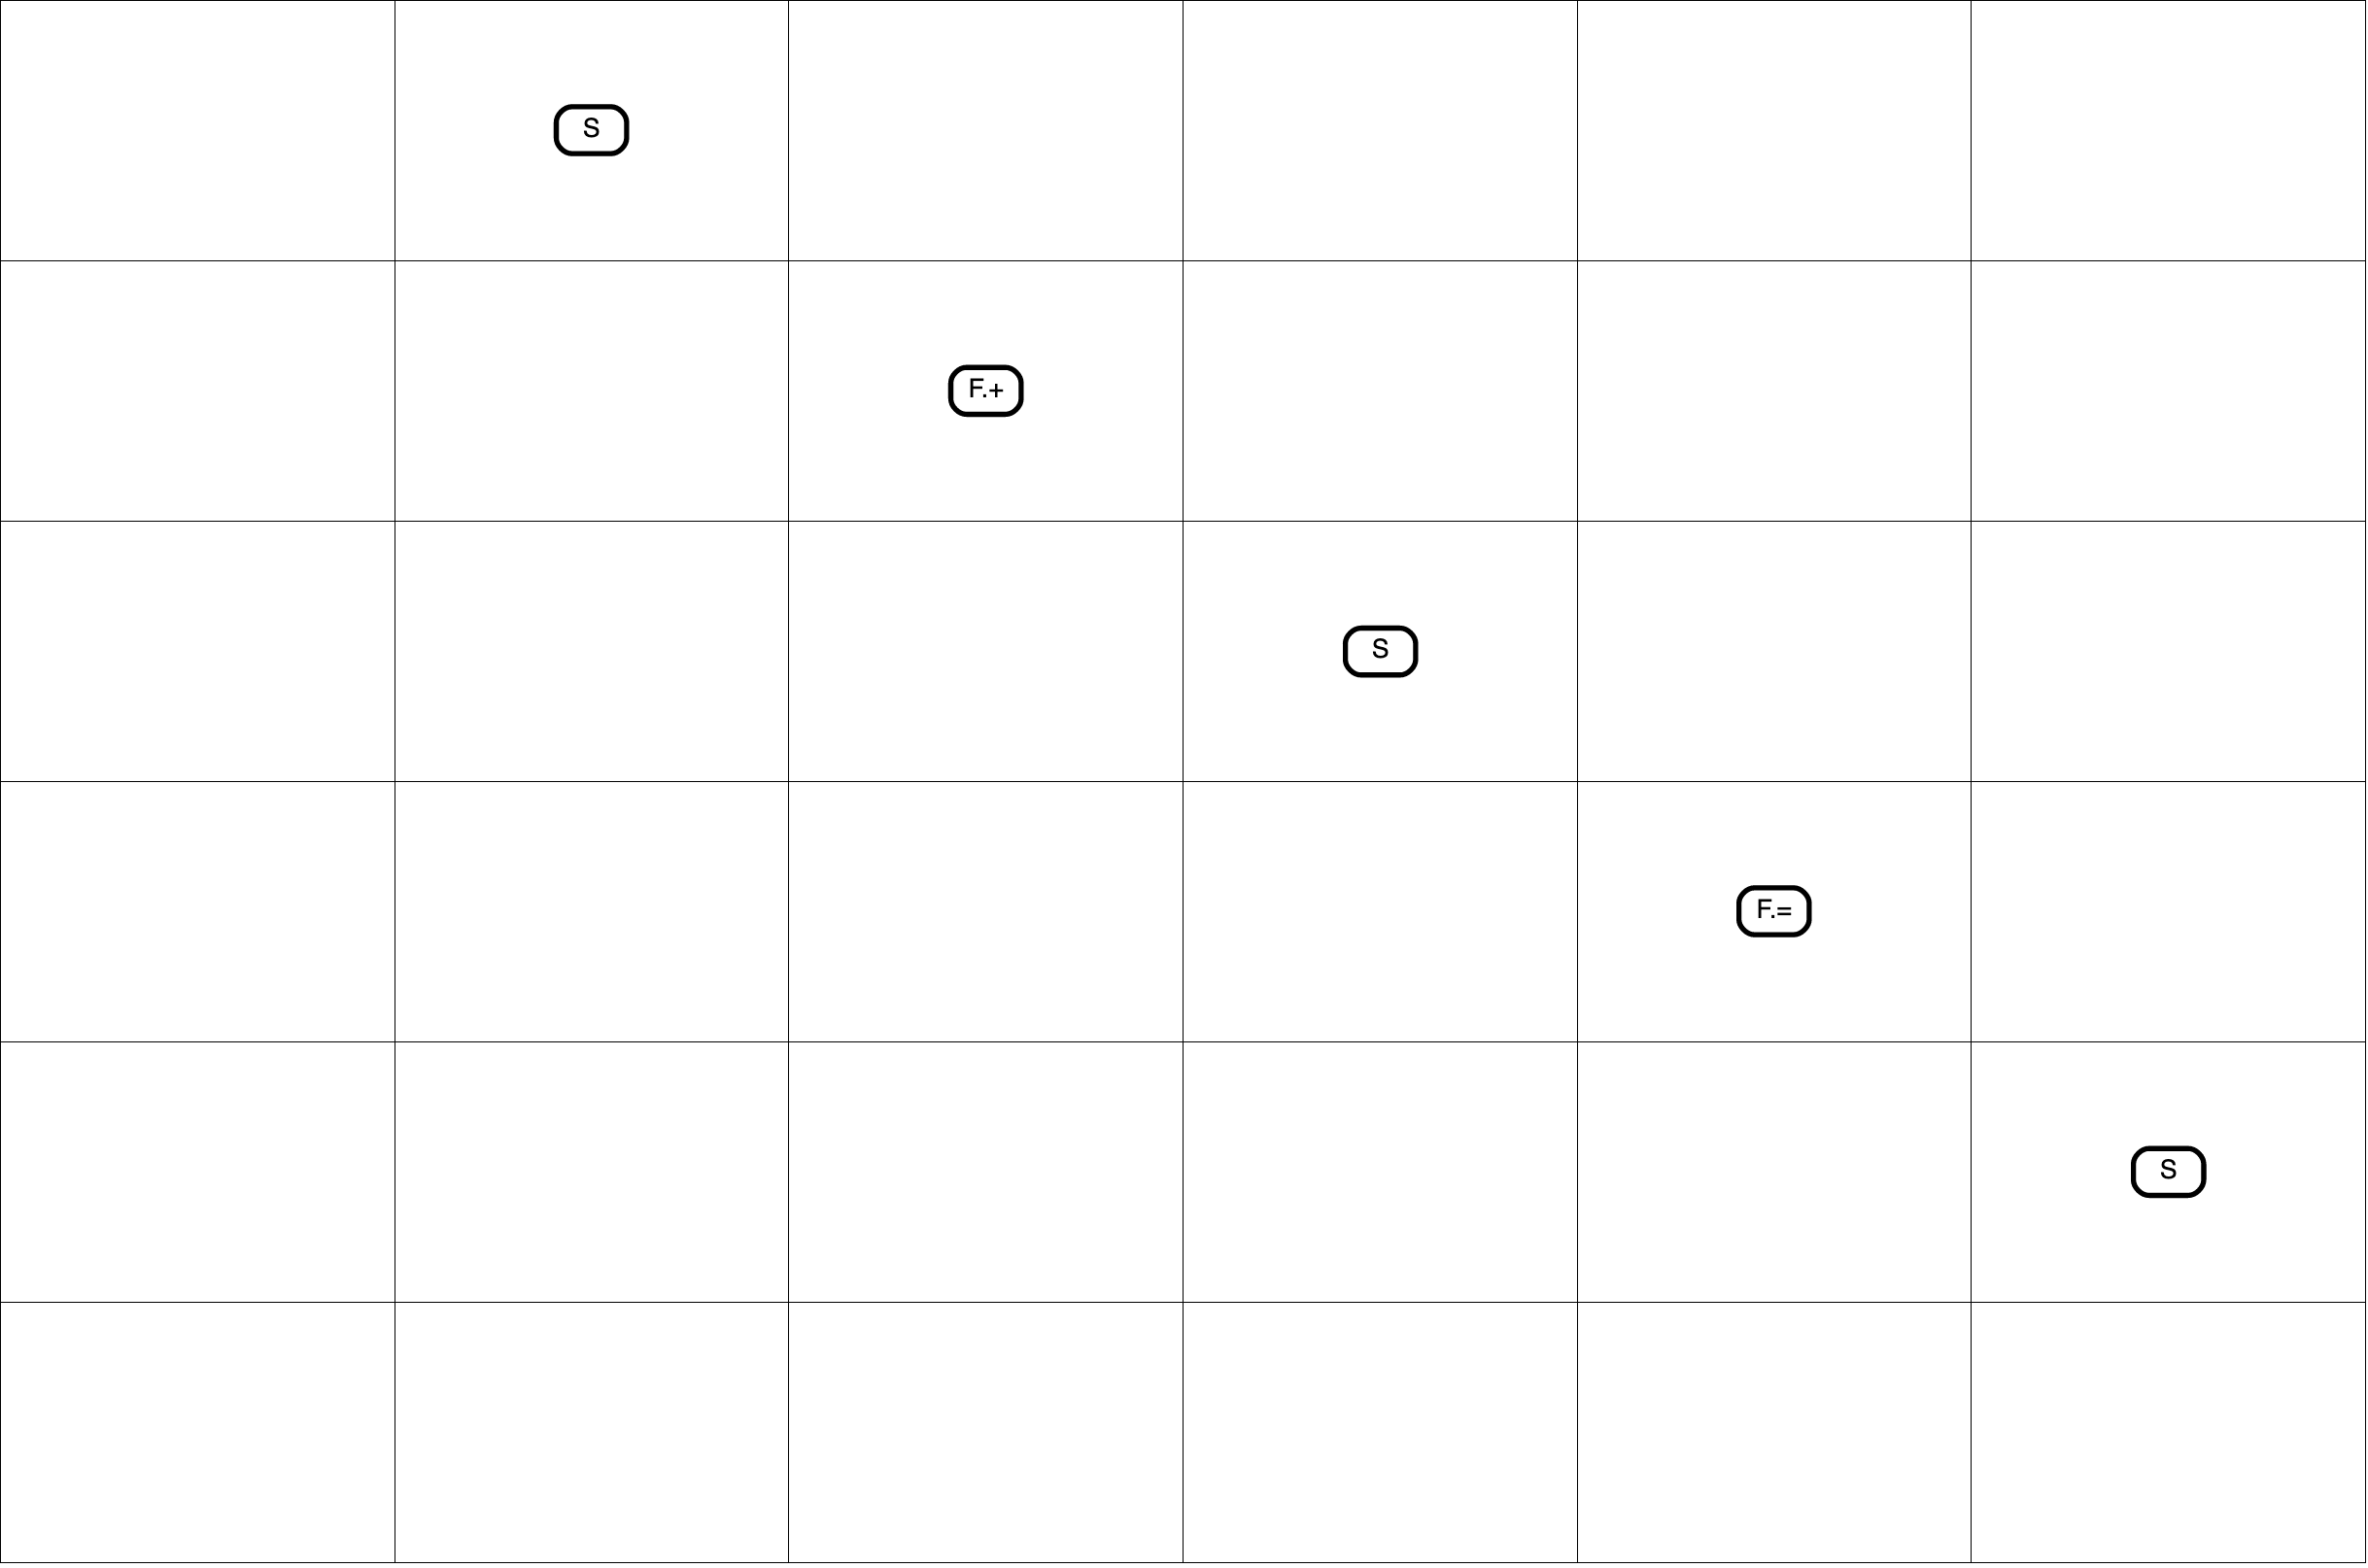
\includegraphics[width=2cm]{../figures/parse1.png}
%%    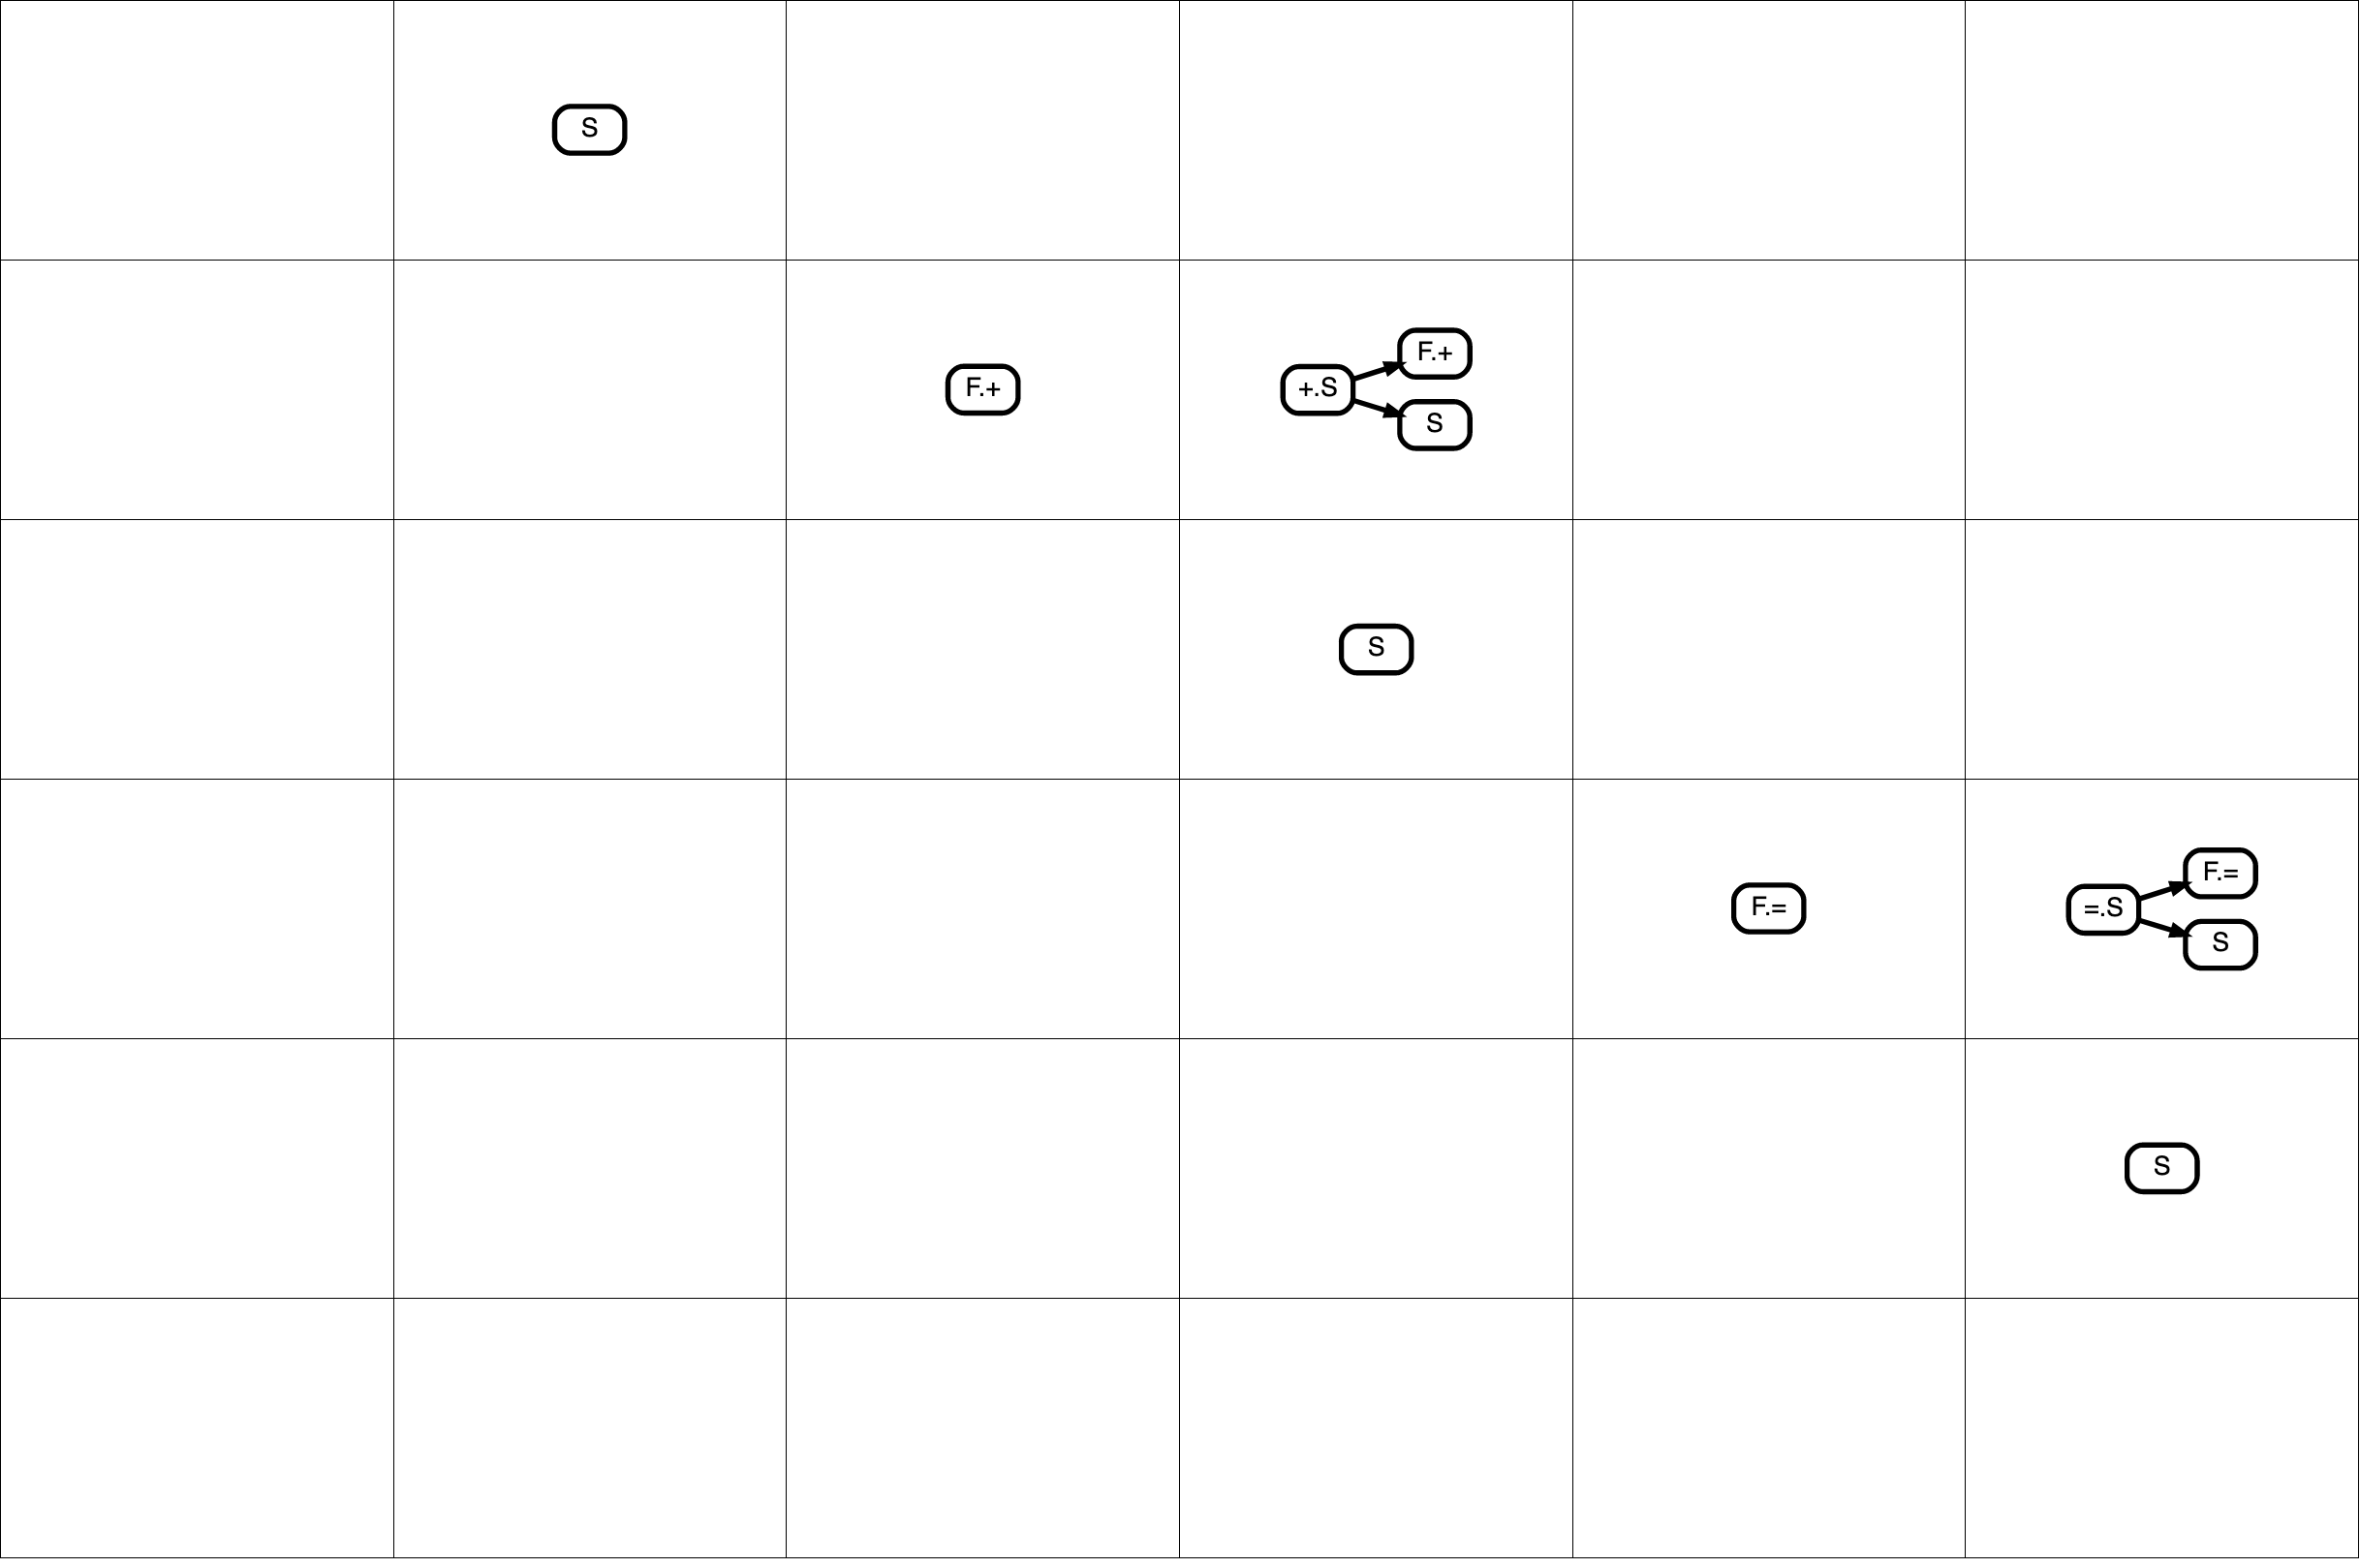
\includegraphics[width=2cm]{../figures/parse2.png}
%%    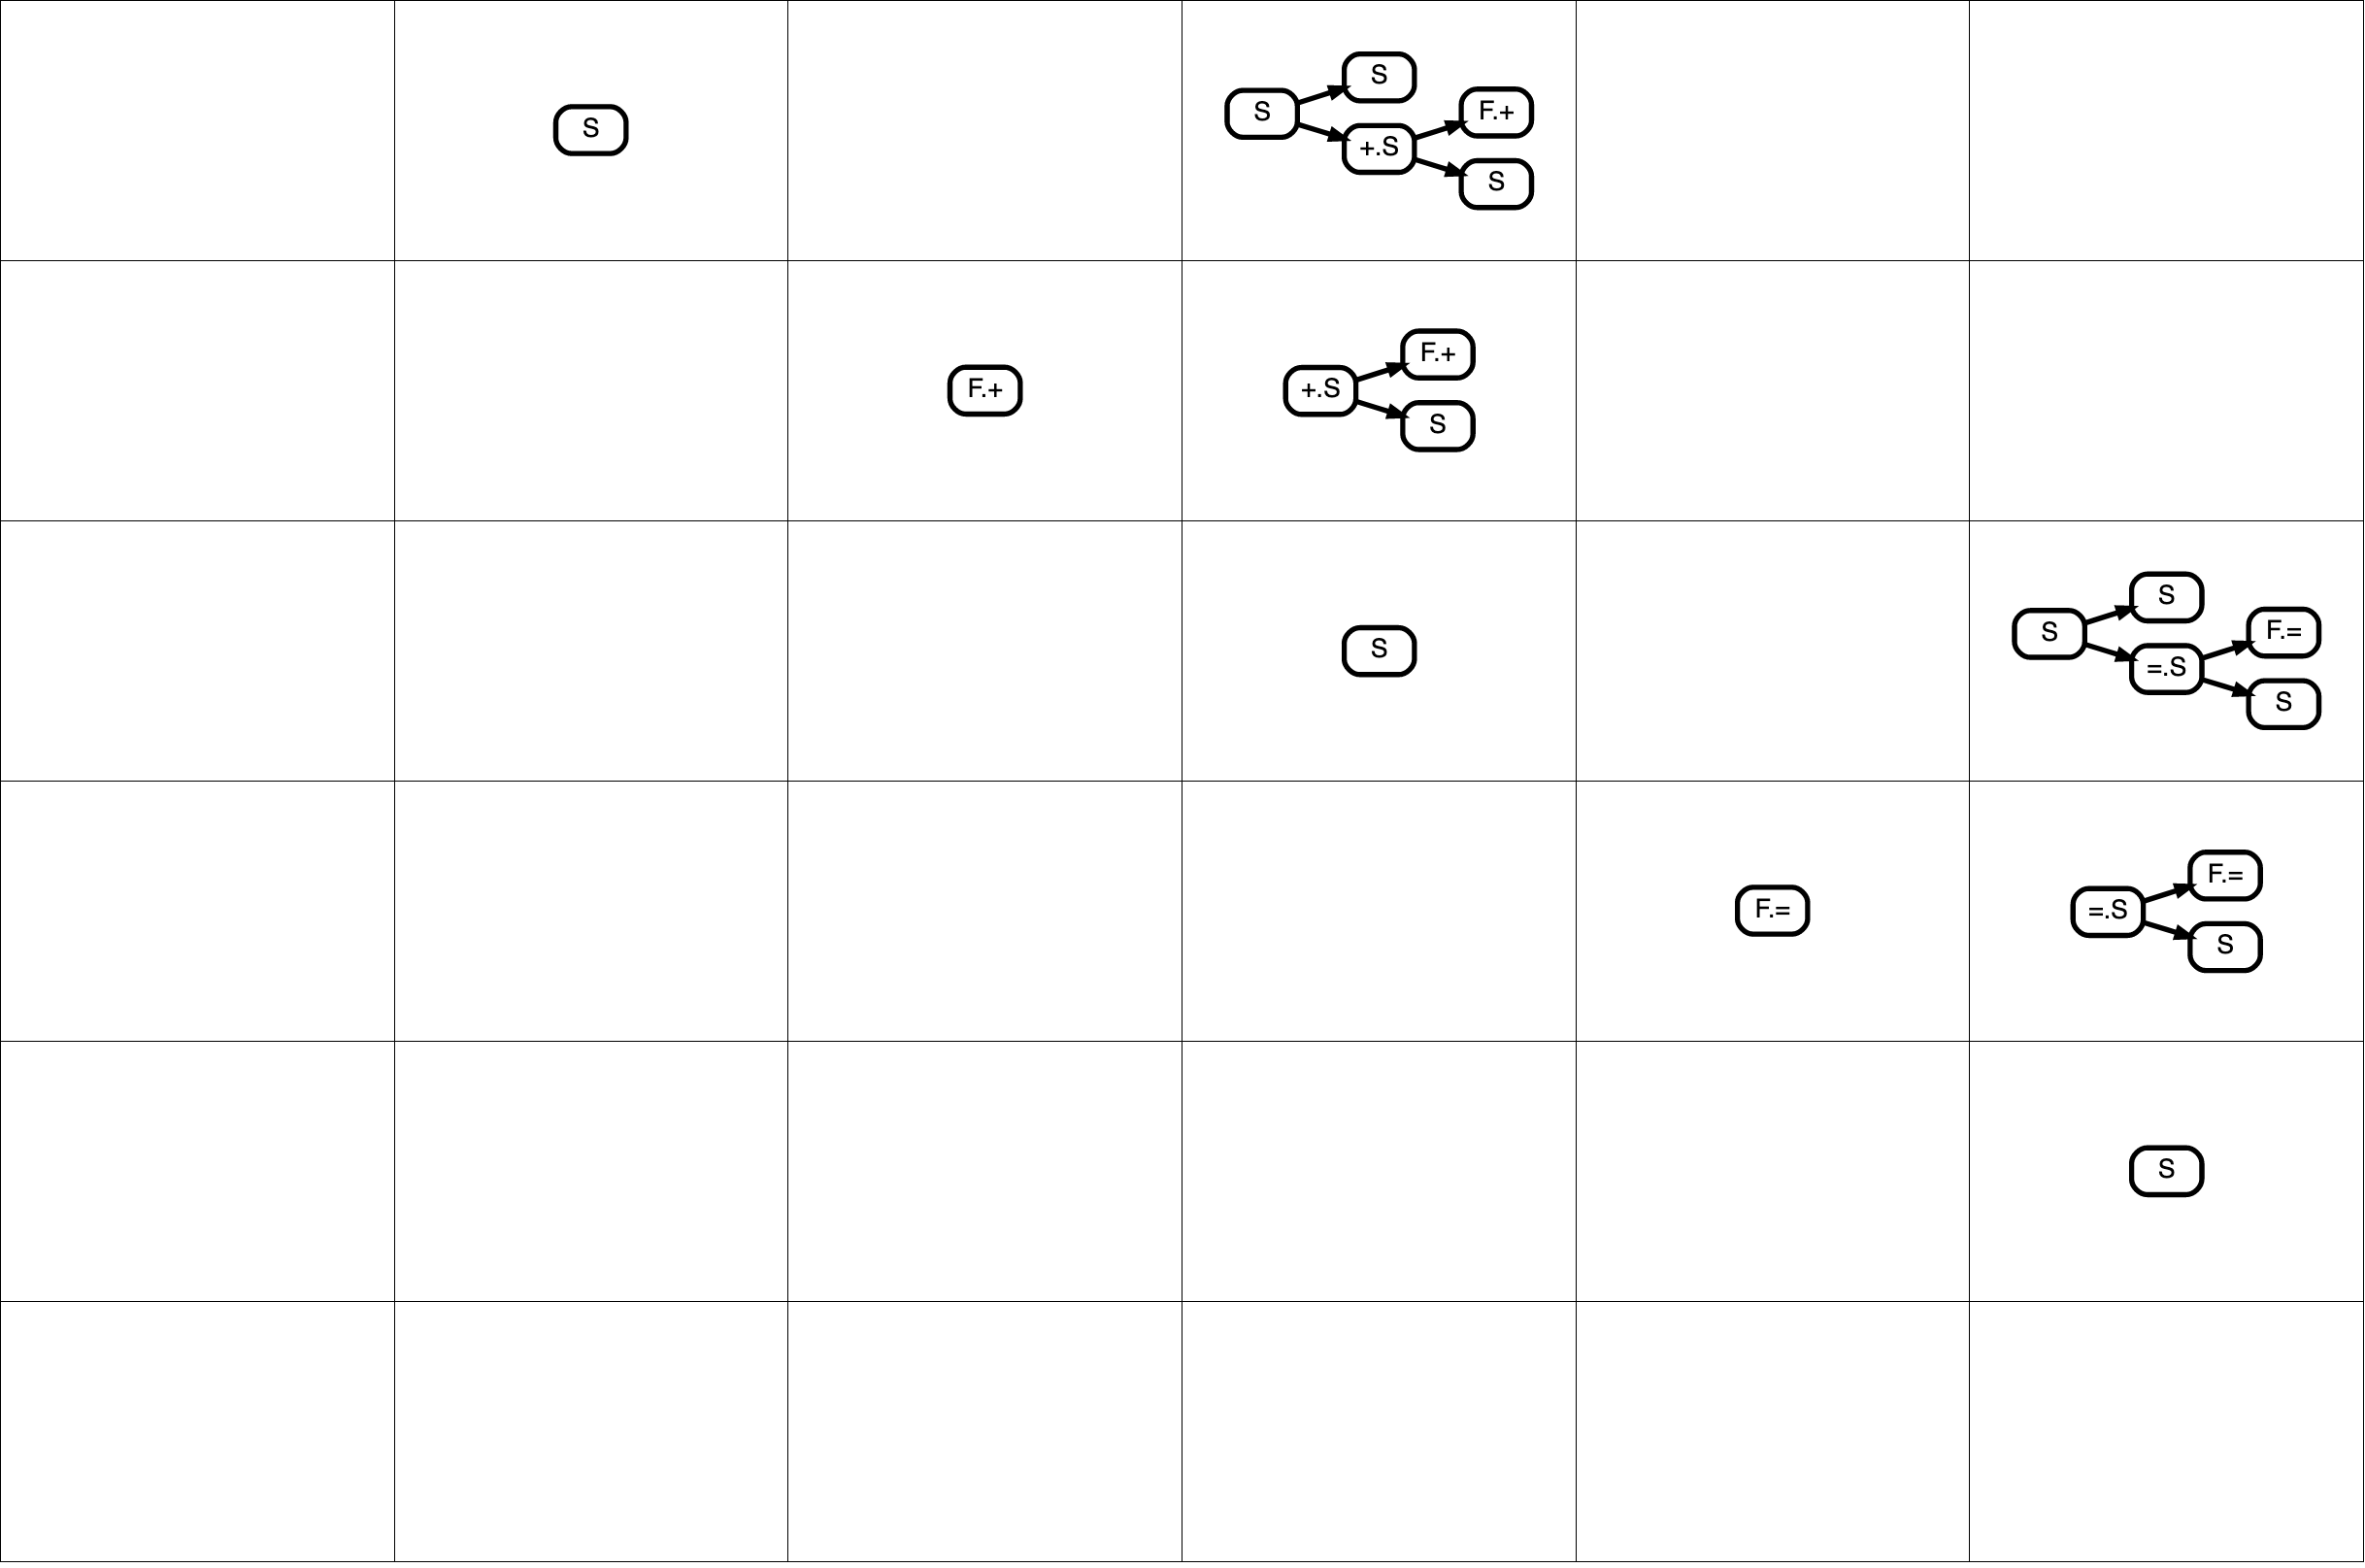
\includegraphics[width=2cm]{../figures/parse3.png}
%%    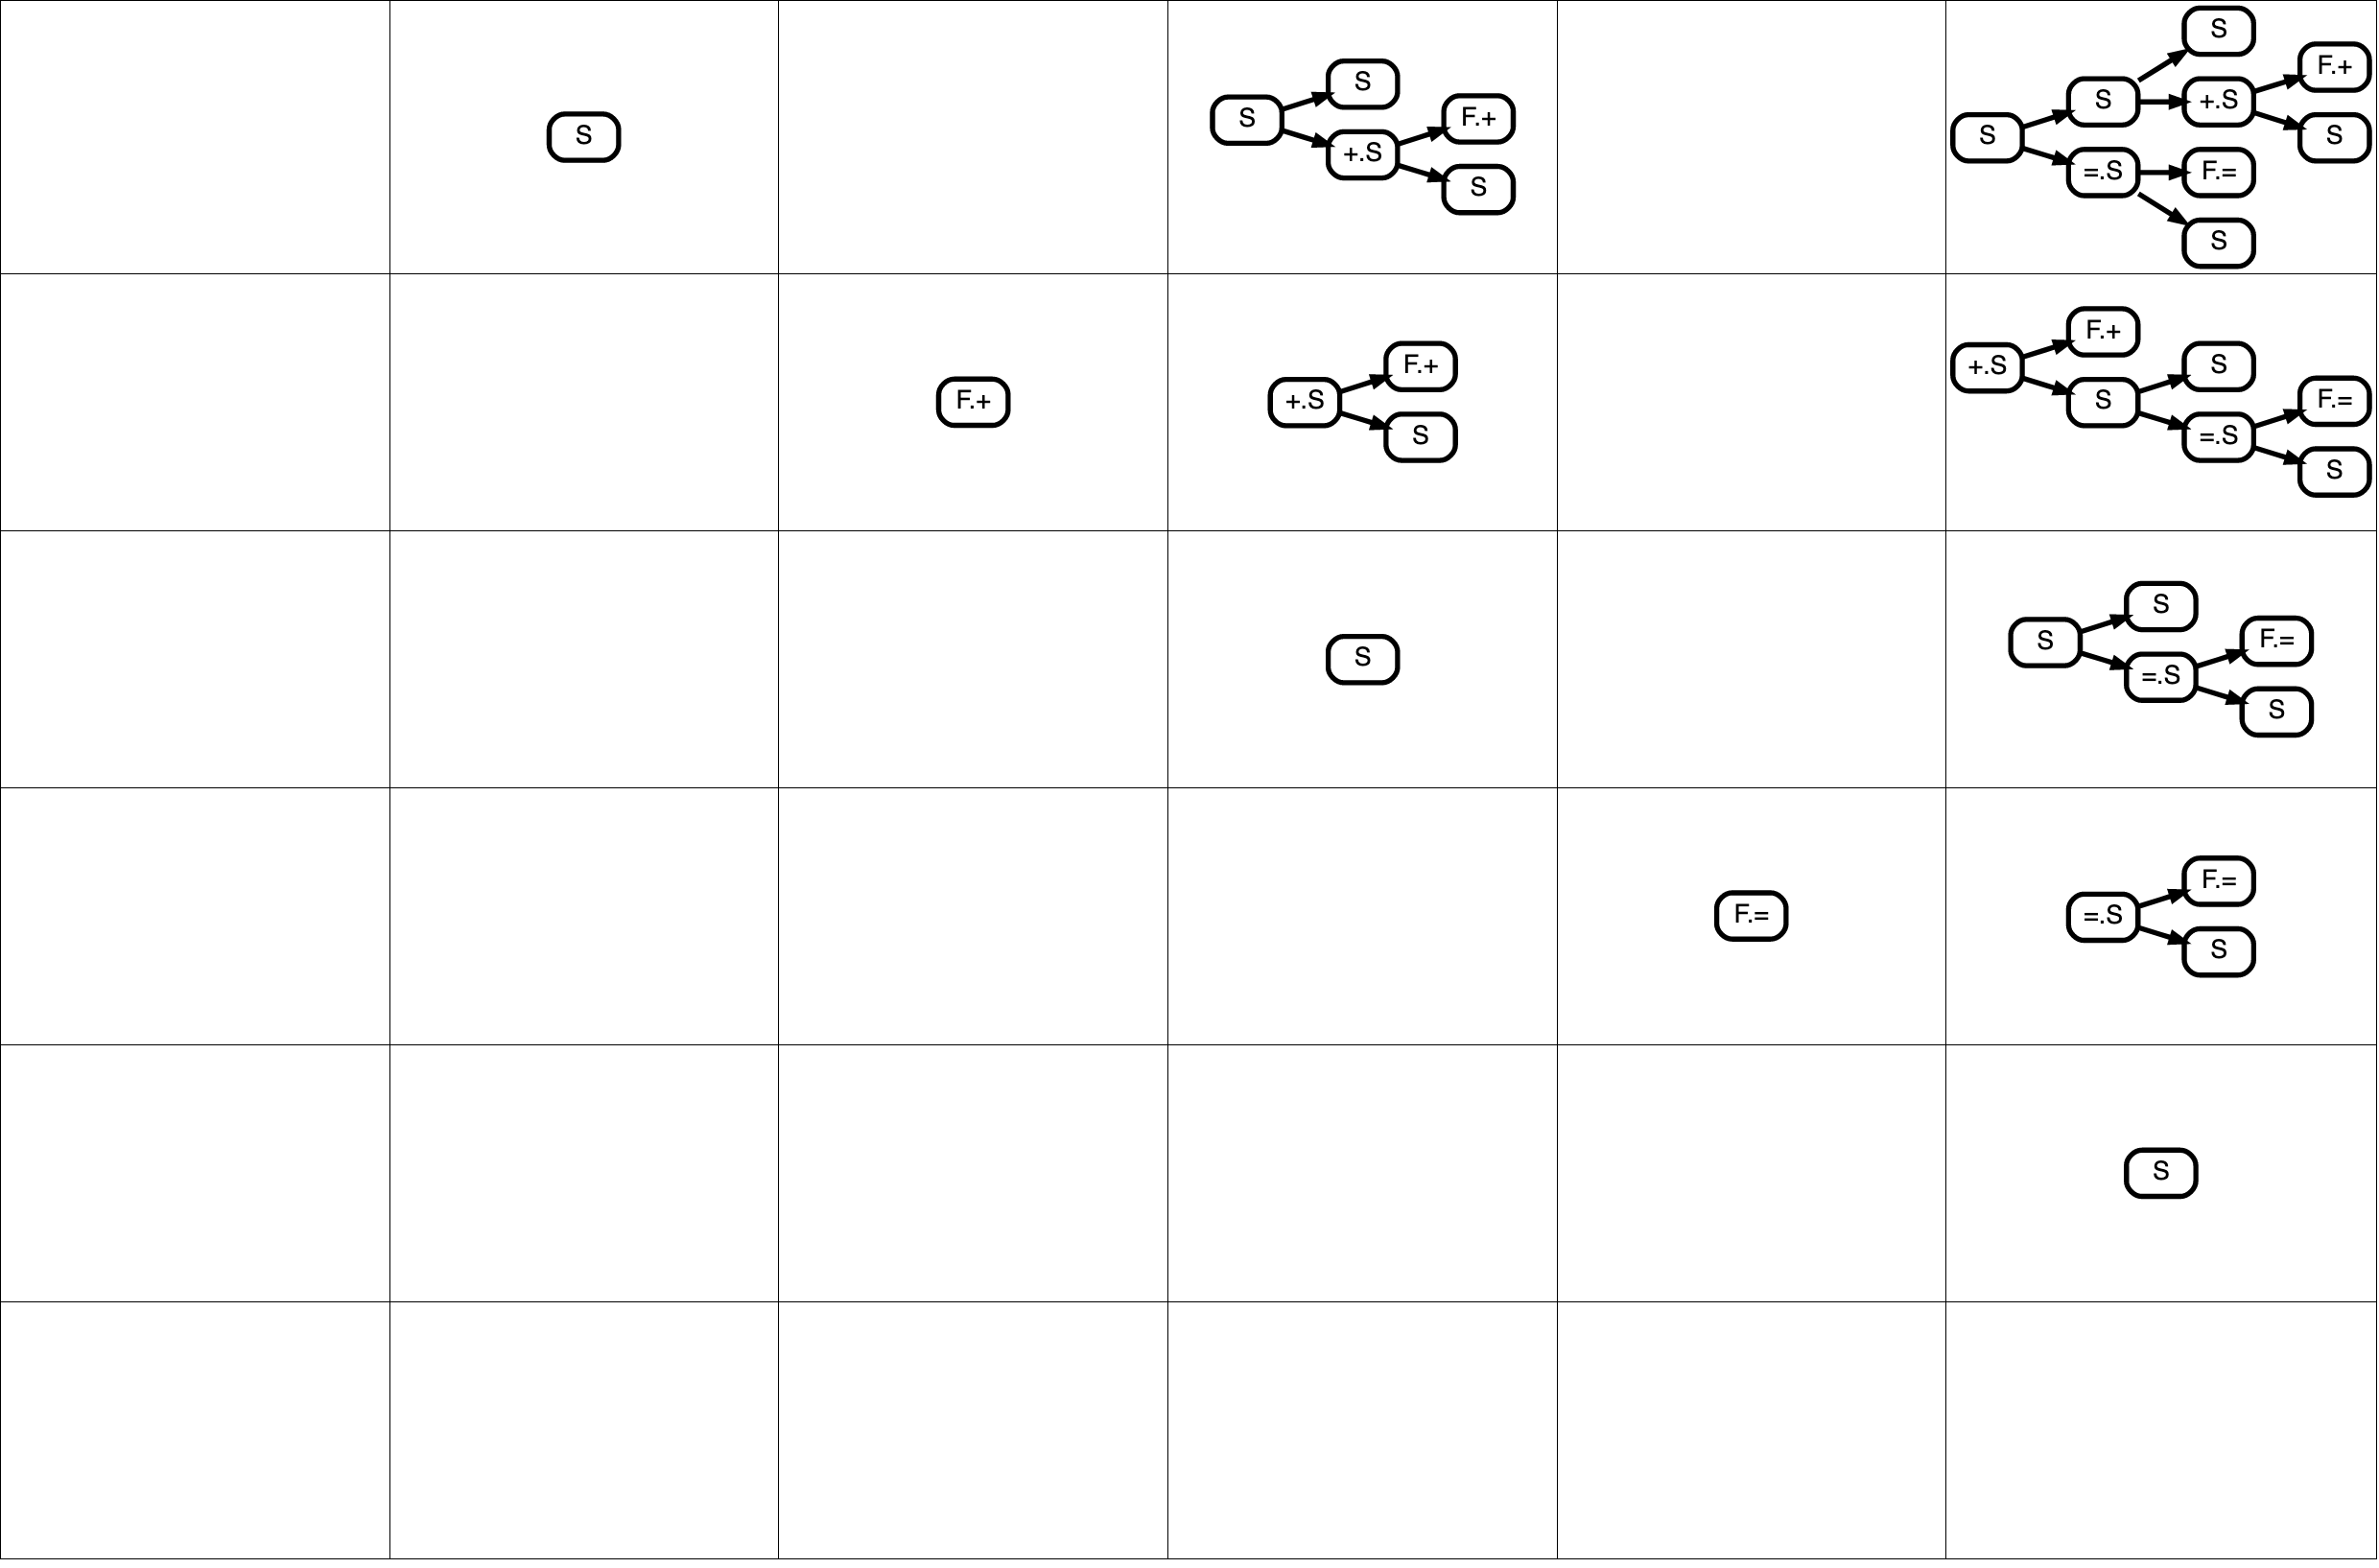
\includegraphics[width=2cm]{../figures/parse4.png}
%%\end{figure}
%
%  \begin{figure}[H]
%    \[
%      \mathcal{M}^* = \begin{pNiceArray}{>{\strut}ccccccc}[margin, extra-margin=2pt,colortbl-like, xdots/line-style=loosely dotted]
%          \vno & \rcr \shup x_1 &  \Cdots      & \mathcal{V}_{1,|x|} & \rcw \mathcal{V}_{1,4} & \cdd & \mathcal{V}^* \\
%          \vdd & \ddd           &  \Ddots      & \rcr\Vdots          & \rcw\vdd               &      & \vdd \\
%               &                &              & \rcr\shup x_{|x|}   & \rcw                   &      & \\
%               &                &              &                     & \mathcal{V}_{4,4}      &      & \\
%               &                &              &                     &                        & \ddd & \\
%               &                &              &                     &                        &      & \mathcal{V}_{n,n} \\
%          \vno & \cdd           &              &                     &                        &      & \vno
%      \end{pNiceArray}
%    \]
%  \end{figure}

%We also need the constraint that no two conflicting nonterminals may be active at any given time... TODO: describe uniqueness constraint
%  \noindent Depicted above is a SAT tensor representing \hlgray{$\sigma_1\:\sigma_2\:\sigma_3$}$\:\_\:\ldots\:\_$ where shaded regions demarcate known bitvector literals $\mathcal{L}_{r,c}$ (i.e., representing established nonterminal forests) and unshaded regions correspond to bitvector variables $\mathcal{V}_{r,c}$ (i.e., representing seeded nonterminal forests to be grown). Since $\mathcal{L}_{r,c}$ are fixed, we precompute them outside the SAT solver.

\section{String Repair}

Given some unparseable string, i.e., $\err{\sigma_1\ldots\:\sigma_n}: \highlight{\Sigma}^n \cap\mathcal{L}(\mathcal{G})^c$, where should we put holes to obtain a parseable $\sigma' \in \mathcal{L}(\mathcal{G})$? To estimate the effect of perturbing $\sigma$ on $\Lambda_\sigma^*$, one can either (1) backpropagate $\nabla S$ across upper-triangular entries of $\mathcal{M}^*$, or (2) stochastically sample \textit{minibatches} $\bm{\sigma}:\Sigma^{n\pm q}\sim\Delta_{q}(\err{\sigma})$ from the Levenshtein q-ball centered on $\err{\sigma}$, i.e., the space of all edits with Levenshtein distance $\leq q$, loosely analogous to a finite difference approximation. In other words, we seek:

\begin{align}
  \bigcup_{\bm{\sigma}\sim\Delta_{k}(\sigma)} \{\sigma' \in \bm{\sigma} \mid S \in \Lambda_{\sigma'}^*\}
\end{align}

Let us consider (2). Suppose $U: \mathbb{Z}_2^{m\times m}$ is a matrix whose structure is shown in Eq.~\ref{eq:lfsr}, wherein $C$ is a primitive polynomial over $\mathbb{Z}_2^m$ with coefficients $C_{1\ldots m}$ and semiring operators $\oplus := \veebar, \otimes := \land$:

\begin{align}
U^tV = \begin{pNiceMatrix}[nullify-dots,xdots/line-style=loosely dotted]
  C_1    & \cdd  &       &       & C_m \\
  \top   & \circ & \cdd  &       & \circ \\
  \circ  & \ddd  & \ddd  &       & \vdd \\
  \vdd   & \ddd  &       &       & \\
  \circ  & \cdd  & \circ & \top  & \circ
\end{pNiceMatrix}^t
\begin{pNiceMatrix}[nullify-dots,xdots/line-style=loosely dotted]
  V_1 \\ \vdd\\ \\ \\ V_m
\end{pNiceMatrix}\label{eq:lfsr}
\end{align}

\noindent Since $C$ is primitive, the sequence $\mathbf{S} = (U^{0 \ldots 2^m-1}V)$ must have \textit{full periodicity}, i.e., for all $i, j \in[0, 2^m)$, $\mathbf{S}_i = \mathbf{S}_j \Rightarrow i = j$. To uniformly sample $\bm\sigma \sim \Sigma^d$ without replacement, we form an injection $\mathbb{Z}_2^m\rightharpoonup\Sigma^d$, cycle over $\mathbf{S}$, then discard samples which index any nonexistent element(s) of $\Sigma$. This method will reject $(1 - |\Sigma|2^{-\lceil\log_2|\Sigma|\rceil})^d$ samples overall, and requires $\mathcal{O}(1)$ per sample and $\mathcal{O}(|\Sigma|^d)$ to cover $\Sigma^d$.

\noindent For example, in order to sample $\mathbf\sigma' \sim \Sigma^2 = \{A, B, C\}^2$, we could use the polynomial $x^4 + x^3 +1$:

\begin{align}
\begin{array}{cccccccccccccc}
  i              & 0          & 1          & 2          & 3          & 4    & 5          & 6    & 7          & 8          & 9     & 10   & 11   \\
  \mathbf{S}_i   & 1000       & 0100       & 0010       & 1001       & 1100 & 0110       & 1011 & 0101       & 1010       & 1101  & 1011 & 0101 \\
  \mathbf\sigma' & \text{C A} & \text{B A} & \text{A C} & \text{C B} &      & \text{B C} &      & \text{B B} & \text{C C} &       &      &
\end{array}
\end{align}

Next, to admit deletion, we augment $P$ with $(\varepsilon^+ \rightarrow \varepsilon \mid \varepsilon^+\:\varepsilon^+)$ and replace each production $(w \rightarrow t)$ with $(w \rightarrow t\:\varepsilon^+ \mid \varepsilon^+\:t \mid t)$.

\begin{center}
  \AxiomC{$\Gamma \vdash \varepsilon \in \Sigma$}
  \RightLabel{$\varepsilon\textsc{-dup}$}
  \UnaryInfC{$\Gamma \vdash (\varepsilon^+ \rightarrow \varepsilon \mid \varepsilon^+\:\varepsilon^+) \in P$}
  \DisplayProof
  \hskip 1.5em
  \AxiomC{$\Gamma \vdash (A \rightarrow B) \in P$}
  \RightLabel{$\varepsilon^+\textsc{-int}$}
  \UnaryInfC{$\Gamma \vdash (A \rightarrow B\:\varepsilon^+ \mid \varepsilon^+\:B \mid B) \in P$}
  \DisplayProof
\end{center}

Finally, to generate $\bm{\sigma}\sim\Delta_{q}(\err{\sigma})$, we enumerate hole configurations $H(\sigma, i) = \sigma_{1\ldots i-1}\:\text{\_ \_}\:\sigma_{i+1\ldots n}$ for each $i \in \stirlingii{n}{d}$ and $d \in 1\ldots q$, then solve for $\mathcal{M}^*$. If $S \in \Lambda^*_{\bm\sigma}?$ has at least one solution, each edit in each $\sigma' \in \bm\sigma$ will match exactly one of seven patterns:\vspace{-10pt}

\begin{align*}
  \text{Deletion}&=\begin{cases}
  \sigma_{1}\:\ldots\:\text{\hlred{$\gamma_1$}\:\hlred{$\gamma_2$}}\:\ldots\:\sigma_n\hspace{0.2cm}\gamma_{1, 2} = \varepsilon\label{eq:del}
  \end{cases}\\
  \text{Substitution}&=\begin{cases}
  \sigma_{1}\:\ldots\:\text{\hlorange{$\gamma_1$}\:\hlred{$\gamma_2$}}\:\ldots\:\sigma_n\hspace{0.2cm}\gamma_1 \neq \varepsilon \land \gamma_2 = \varepsilon\\
  \sigma_{1}\:\ldots\:\text{\hlred{$\gamma_1$}\:\hlorange{$\gamma_2$}}\:\ldots\:\sigma_n\hspace{0.2cm}\gamma_1 = \varepsilon \land \gamma_2 \neq \varepsilon\\
  \sigma_{1}\:\ldots\: \text{\hlorange{$\gamma_1$}\:\hlorange{$\gamma_2$}}\:\ldots\:\sigma_n\hspace{0.2cm}\{\gamma_1, \gamma_2\}\cap\{\varepsilon, \sigma_i\} = \varnothing
  \end{cases}\\
  \text{Insertion}&=\begin{cases}
  \sigma_{1}\:\ldots\: \text{\hlgreen{$\gamma_1$}\:\hlorange{$\gamma_2$}}\:\ldots\:\sigma_n\hspace{0.2cm}\gamma_1 = \sigma_i \land \gamma_2 \notin \{\varepsilon,  \sigma_i\}\label{eq:ins2}\\
  \sigma_{1}\:\ldots\: \text{\hlorange{$\gamma_1$}\:\hlgreen{$\gamma_2$}}\:\ldots\:\sigma_n\hspace{0.2cm}\gamma_1 \notin \{\varepsilon, \sigma_i\} \land \gamma_2 = \sigma_i\label{eq:ins1}\\
  \sigma_{1}\:\ldots\: \text{\hlgreen{$\gamma_1$}\:\hlgreen{$\gamma_2$}}\:\ldots\:\sigma_n\hspace{0.2cm}\gamma_{1,2} = \sigma_i\label{eq:copy}
  \end{cases}
\end{align*}

\noindent This approach is tractable for $n \lesssim 100, q \lesssim 3$, however more complex repairs require a more efficient gradient estimator. As SAT encoding incurs a fixed penalty, for small repairs, we have observed it is more efficient to enumerate all sketch templates and solve for admissible repairs outside the SAT solver.

%  This constitutes to a top-down inference procedure, in which, following the tradition of Bird and Meertens, we define the exponential of a forest as a nested datatype called a \textit{taiga}:
%
%  \begin{align*}
%    \text{\textbf{data} \textit{Tree} } a &= \varnothing \mid \langle a, \langle\textit{Tree a, Tree a}\rangle\rangle\\
%    \text{\textbf{data} \textit{Forest} } a &= \varnothing \mid \langle \{a\}, \{\langle\textit{Forest a,  Forest a}\rangle\}\rangle\\
%    \text{\textbf{data} \textit{Taiga} } a &= \varnothing \mid \langle a, [\langle\textit{Taiga (Taiga a)}\rangle^2]\rangle
%  \end{align*}
%
%  This is needed because of the doubly-ambiguous nature of tree search: a single string may have a parse forest, and an incomplete string simultaneously occupies a superposition of possible parse forests. When we encounter two adjacent parse forests which cannot be joined, we know that either (1) the left derivation must change (2) the right derivation must change or (3) there must be a hole in the middle which joins the two together. When recursing over the state space, we must simultaneously consider all three possibilities.

\section{Context-sensitive reachability}

It is well-known that the family of CFLs is not closed under intersection. For example, consider $\mathcal{L}_\cap := \mathcal{L}(\mathcal{G}_1) \cap \mathcal{L}(\mathcal{G}_1)$:

\begin{table}[H]
\begin{tabular}{llll}
  $P_1 := \big\{\;S \rightarrow L R,$ & $L \rightarrow a b \mid a L b,$ & $R \rightarrow c \mid c R\;\big\}$\vspace{5pt}\\
  $P_2 := \big\{\;S \rightarrow L R,$ & $R \rightarrow b c \mid b R c,$ & $L \rightarrow a \mid a L\;\big\}$
\end{tabular}
\end{table}

\noindent Note that $\mathcal{L}_\cap$ generates the language $\big\{\;a^d b^d c^d \mid d > 0\;\big\}$, which according to the pumping lemma is not context-free. We can encode $\bigcap_{i=1}^c \mathcal{L}(\mathcal{G}_i)$ as a polygonal prism with upper-triangular matrices adjoined to each rectangular face. More precisely, we intersect all terminals $\Sigma_\cap := \bigcap_{i=1}^c \Sigma_i$, then for each $t_\cap \in \Sigma_\cap$ and CFG, construct an equivalence class $E(t_\cap, \mathcal{G}_i) = \{ w_i \mid (w_i \rightarrow t_\cap) \in P_i\}$ and bind them together:\vspace{-5pt}

\begin{align}
  \bigwedge_{t\in\Sigma_\cap}\bigwedge_{j = 1}^{c-1}\bigwedge_{i=1}^{|\sigma|} E(t_{\cap}, \mathcal{G}_j) \equiv_{\sigma_i} E(t_{\cap}, \mathcal{G}_{j+1})
\end{align}
  % Generated by cfl4_intersection.vox, open with https://voxelator.com/
\begin{figure}[H]
  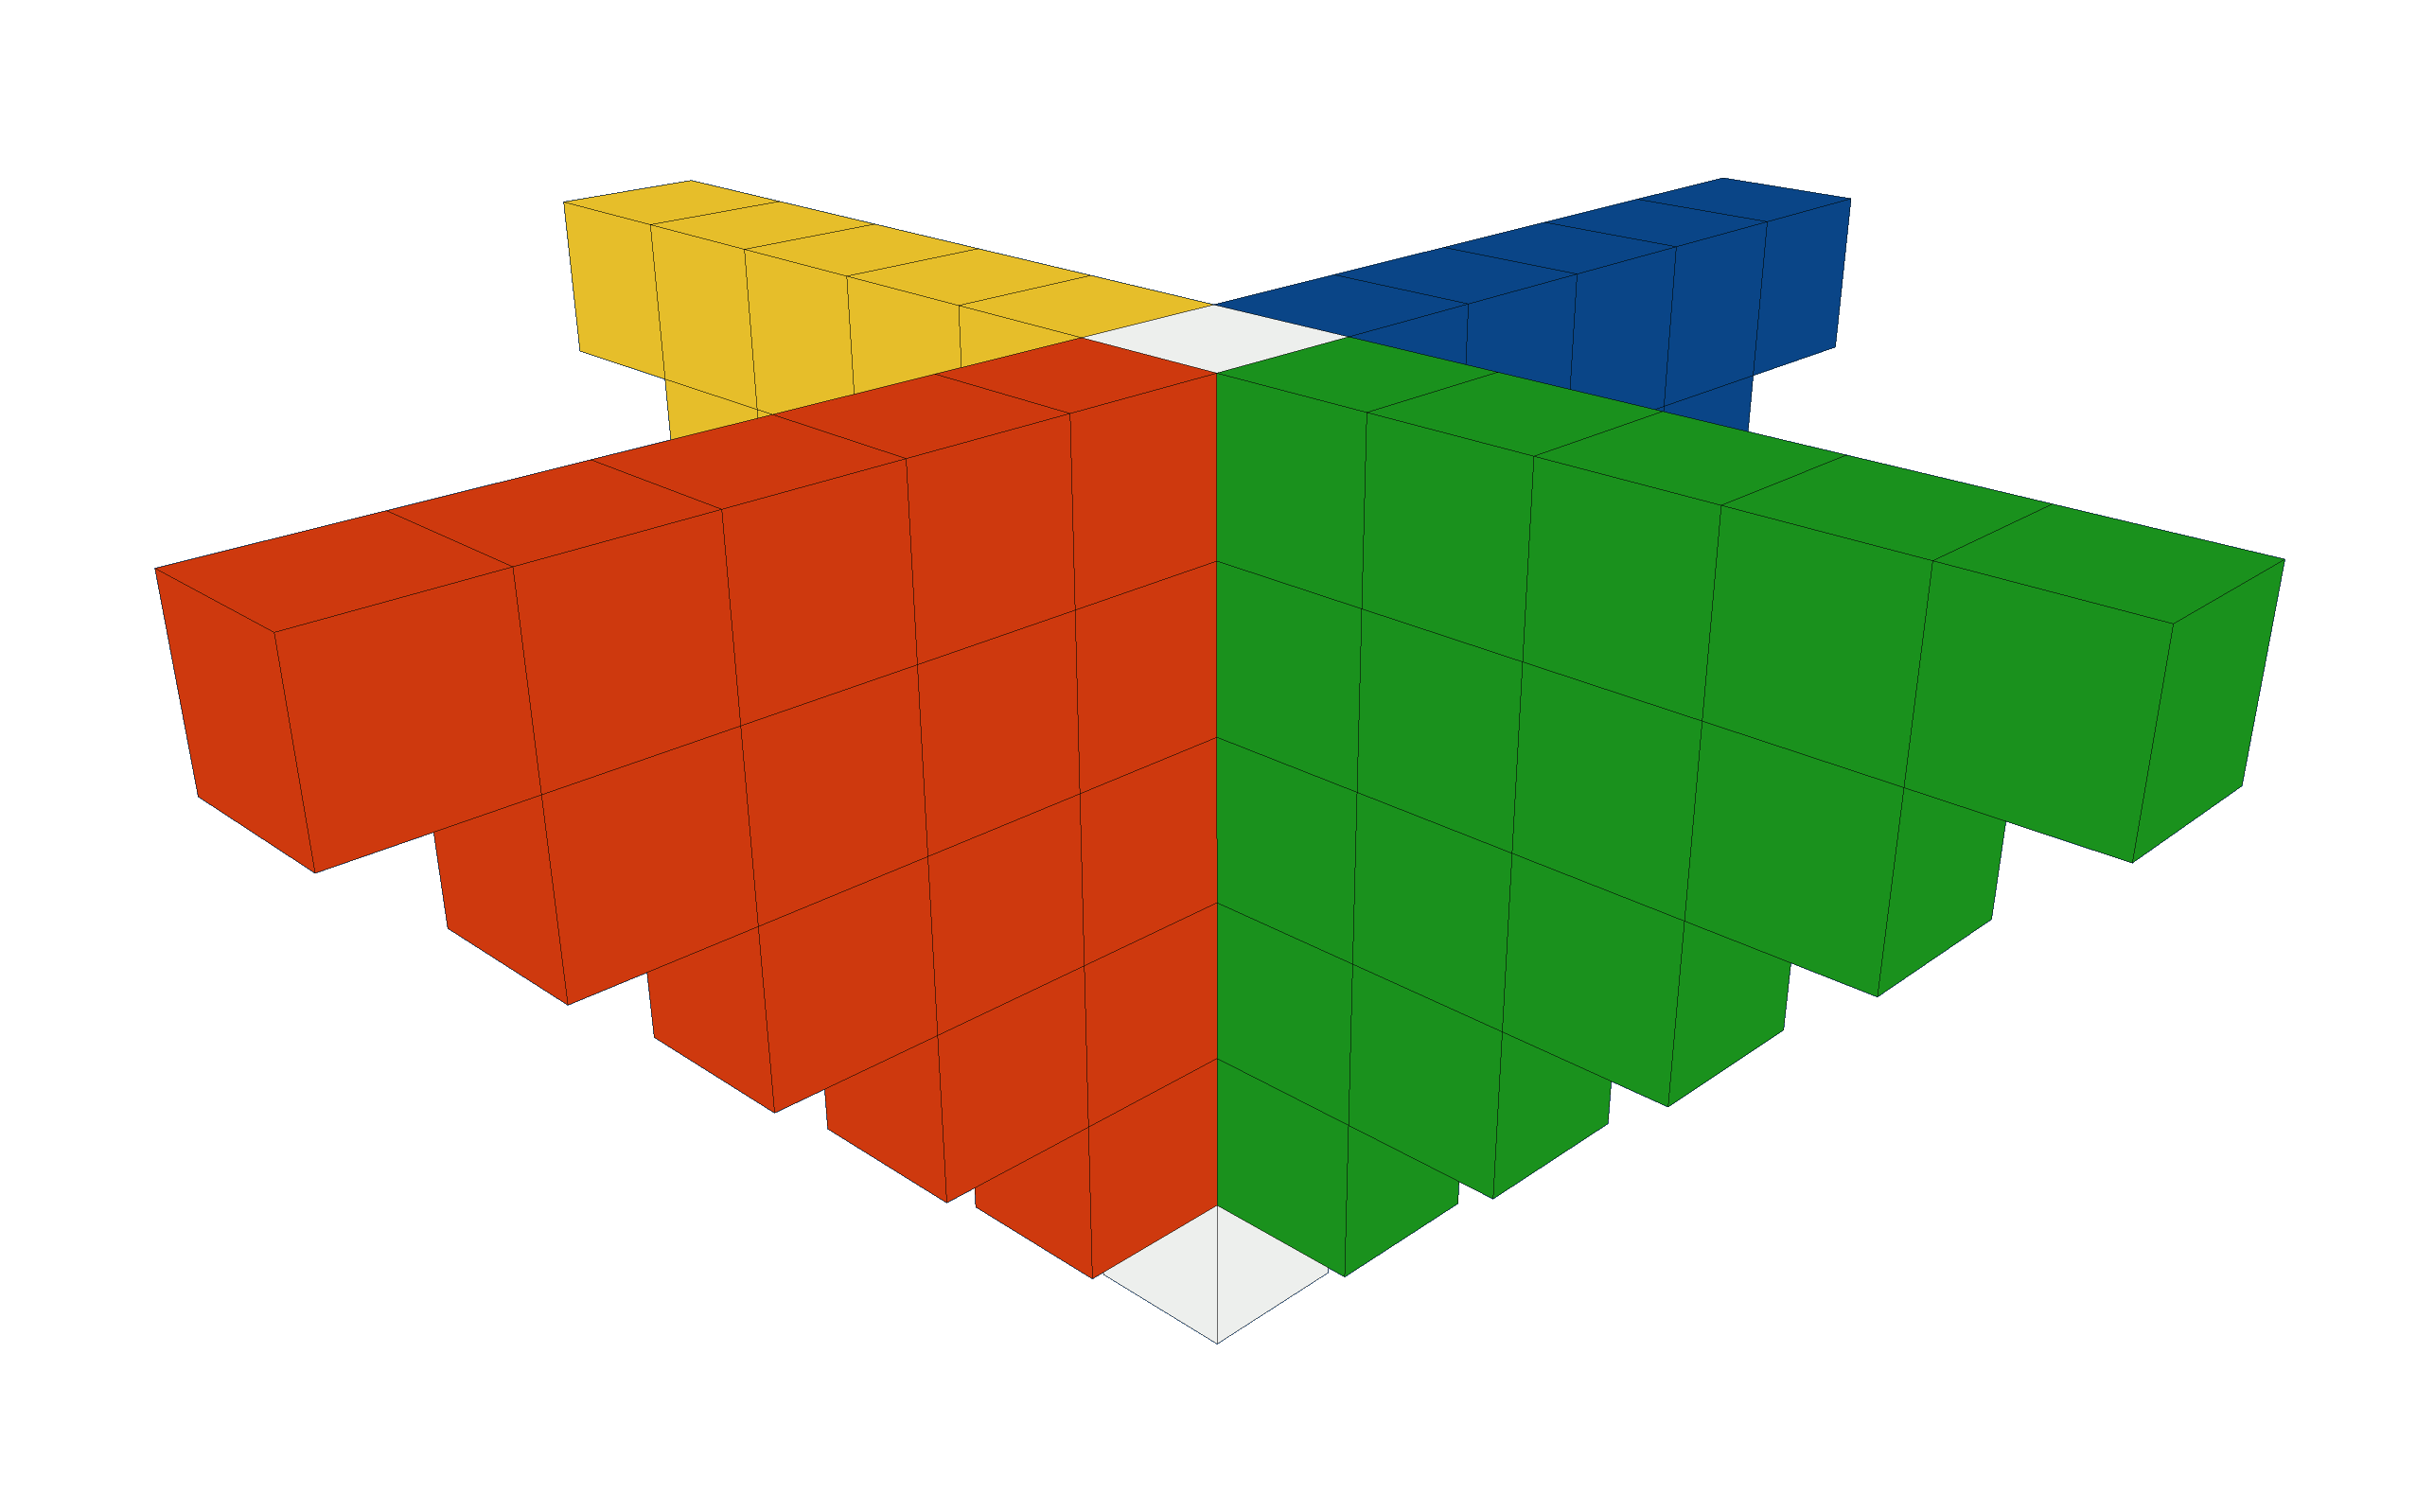
\includegraphics[height=0.1\textwidth]{../figures/angle1.png}\hspace{-5pt}
  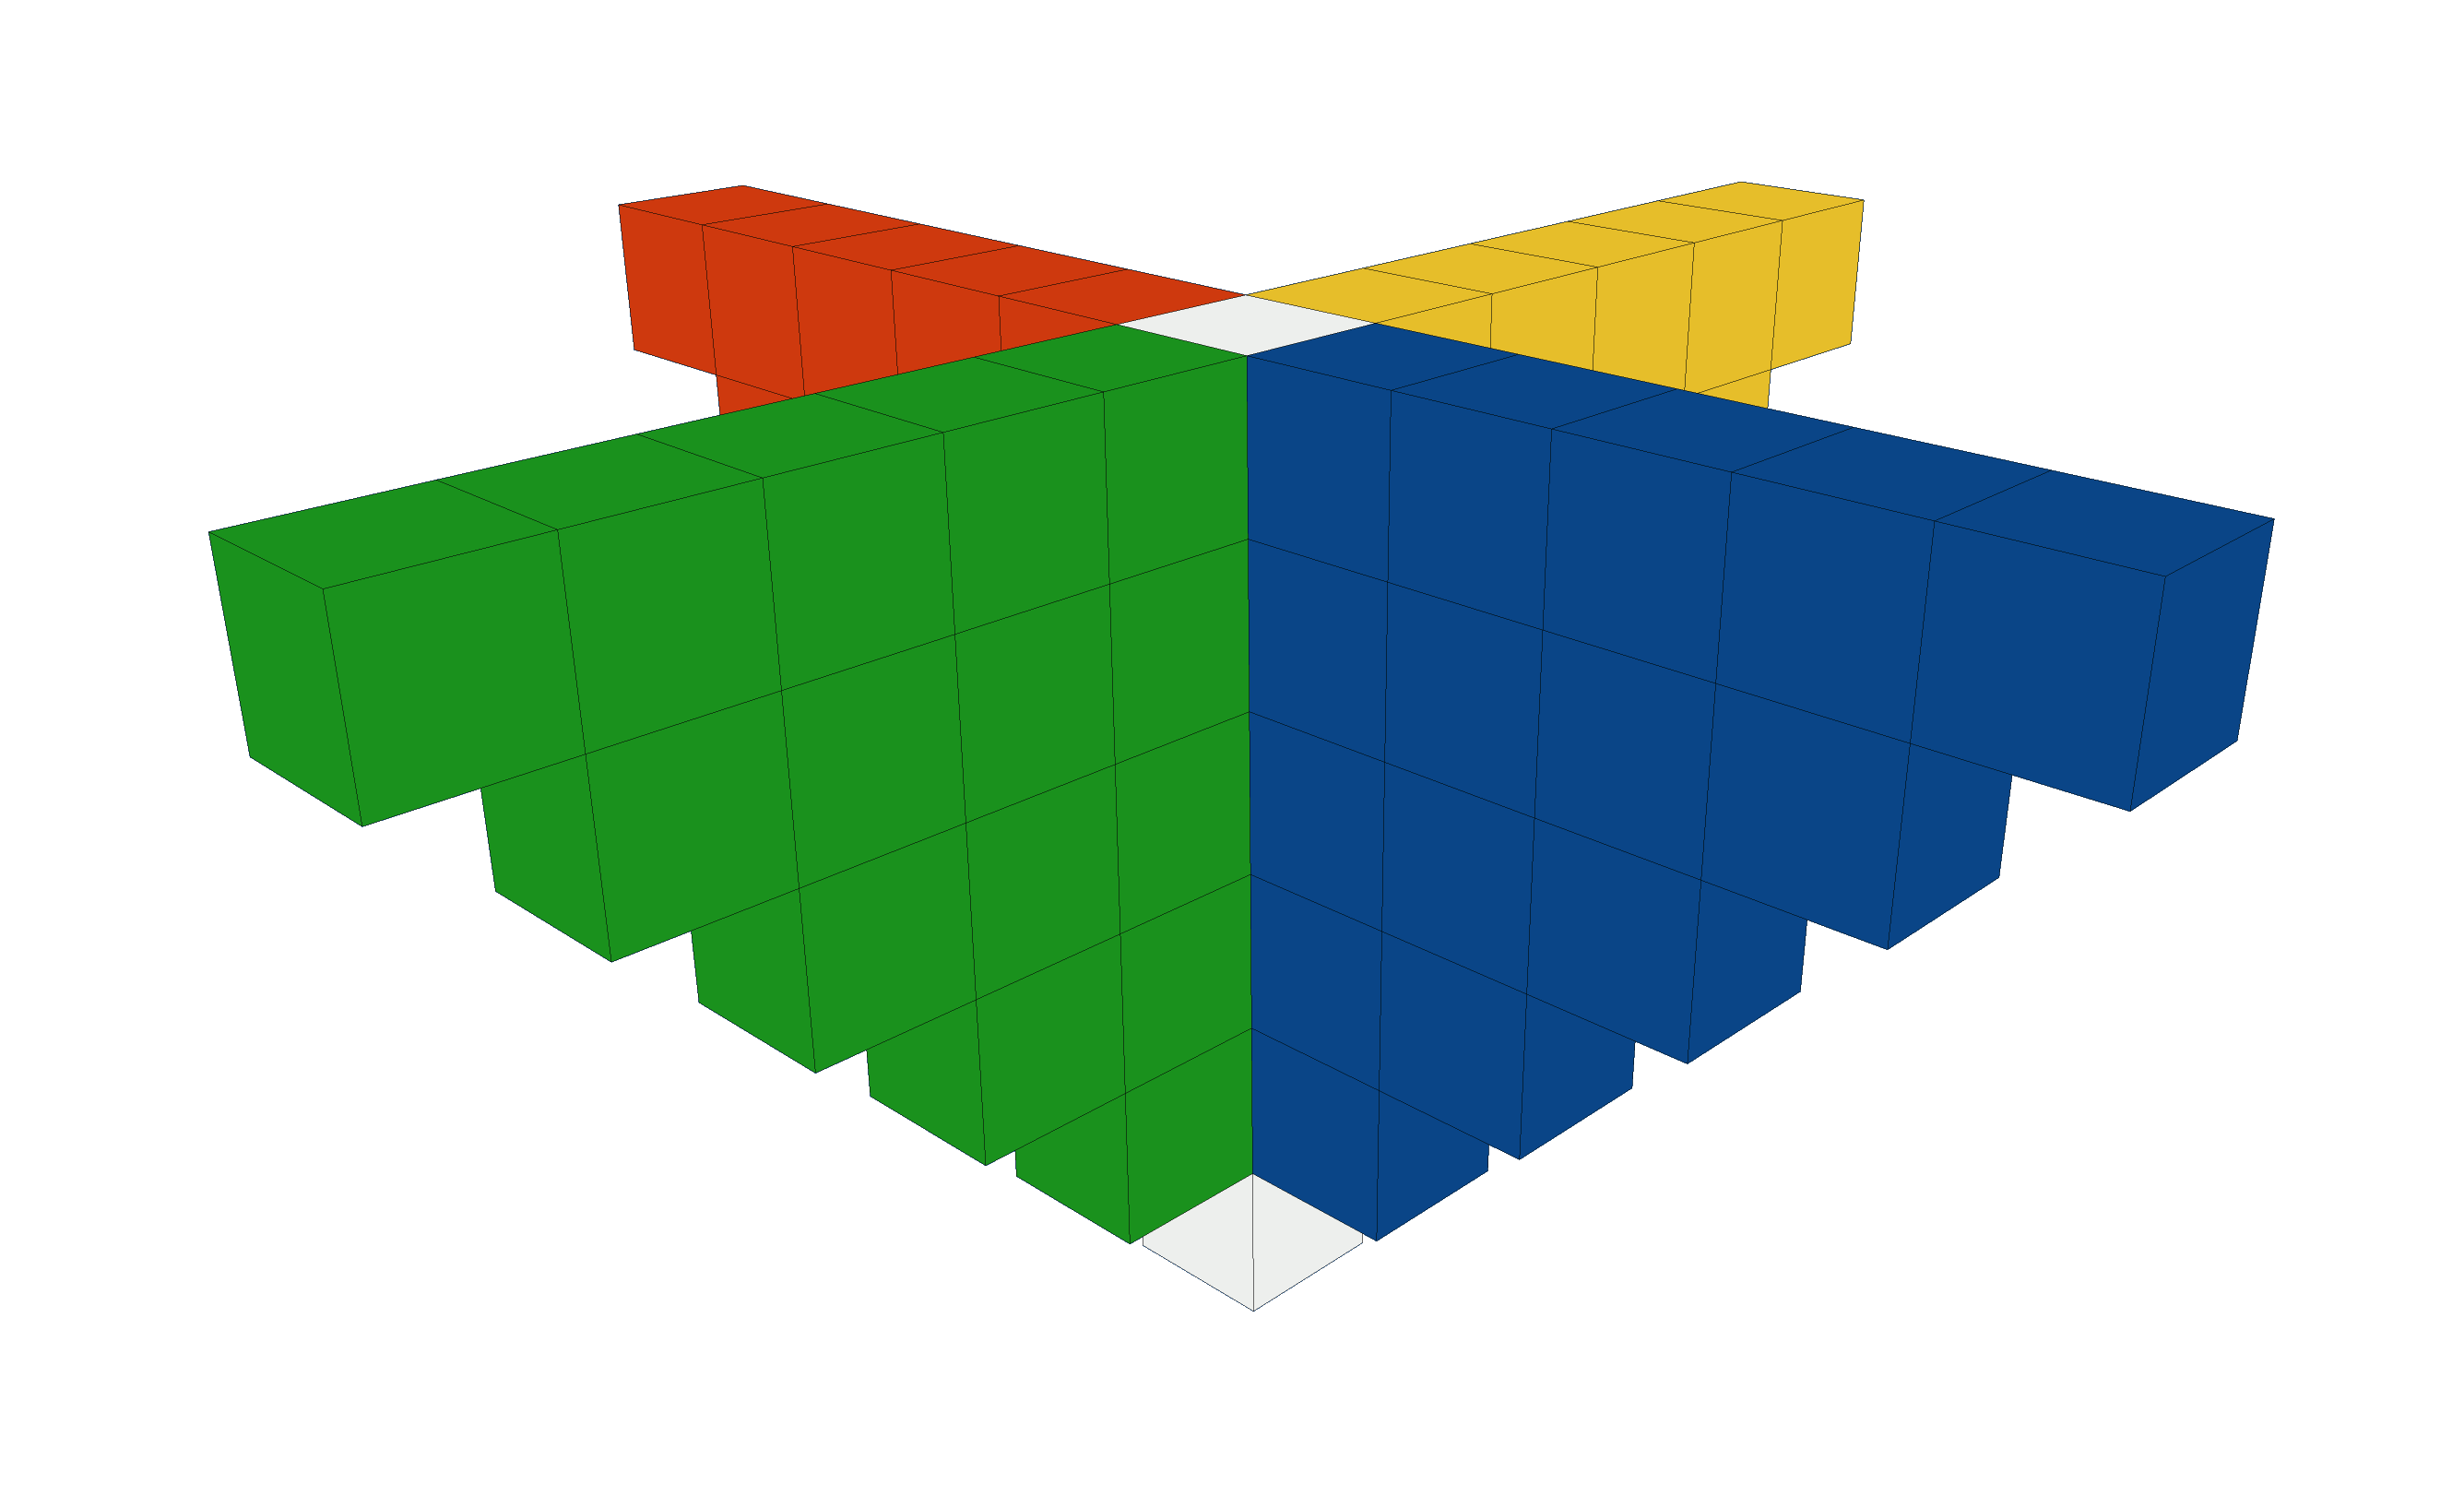
\includegraphics[height=0.1\textwidth]{../figures/angle2.png}\hspace{-5pt}
  
\includegraphics[height=0.1\textwidth]{../figures/angle5.png}\hspace{-5pt}
  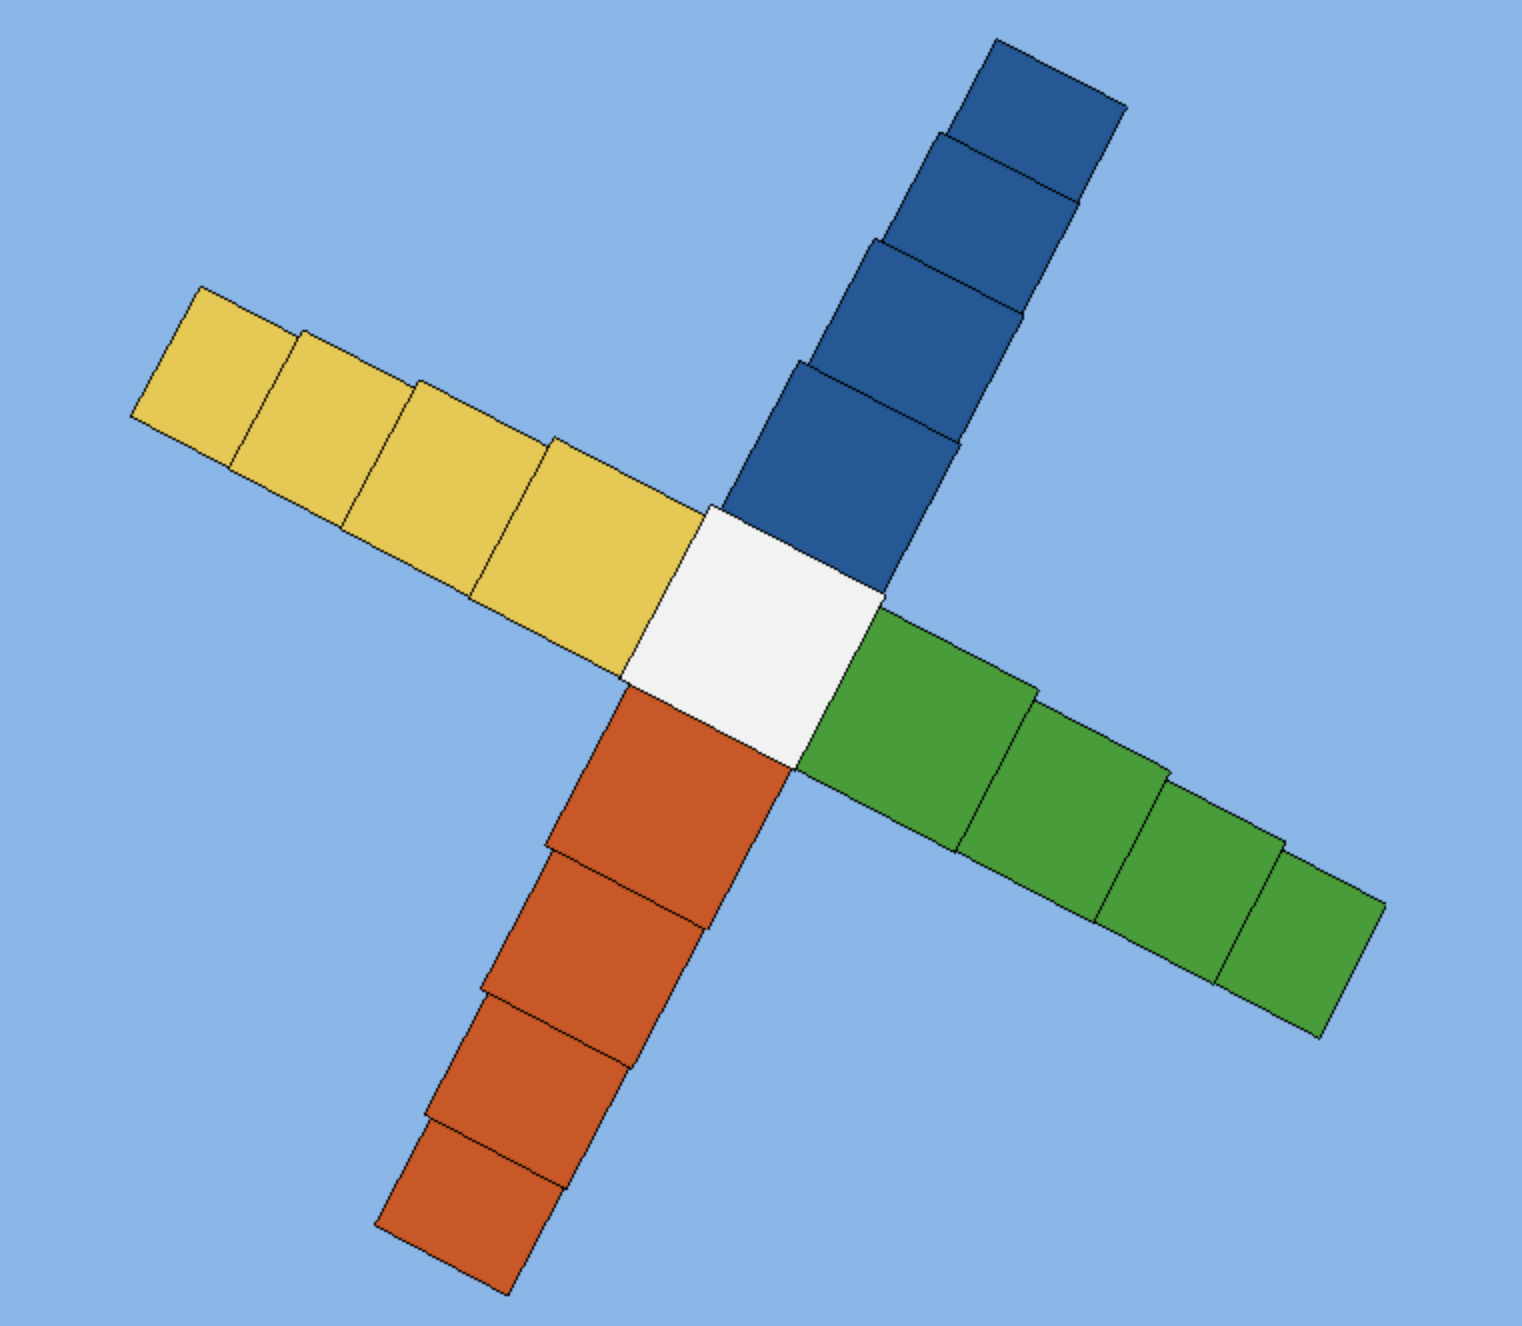
\includegraphics[height=0.1\textwidth]{../figures/angle3.png}\hspace{-3pt}
  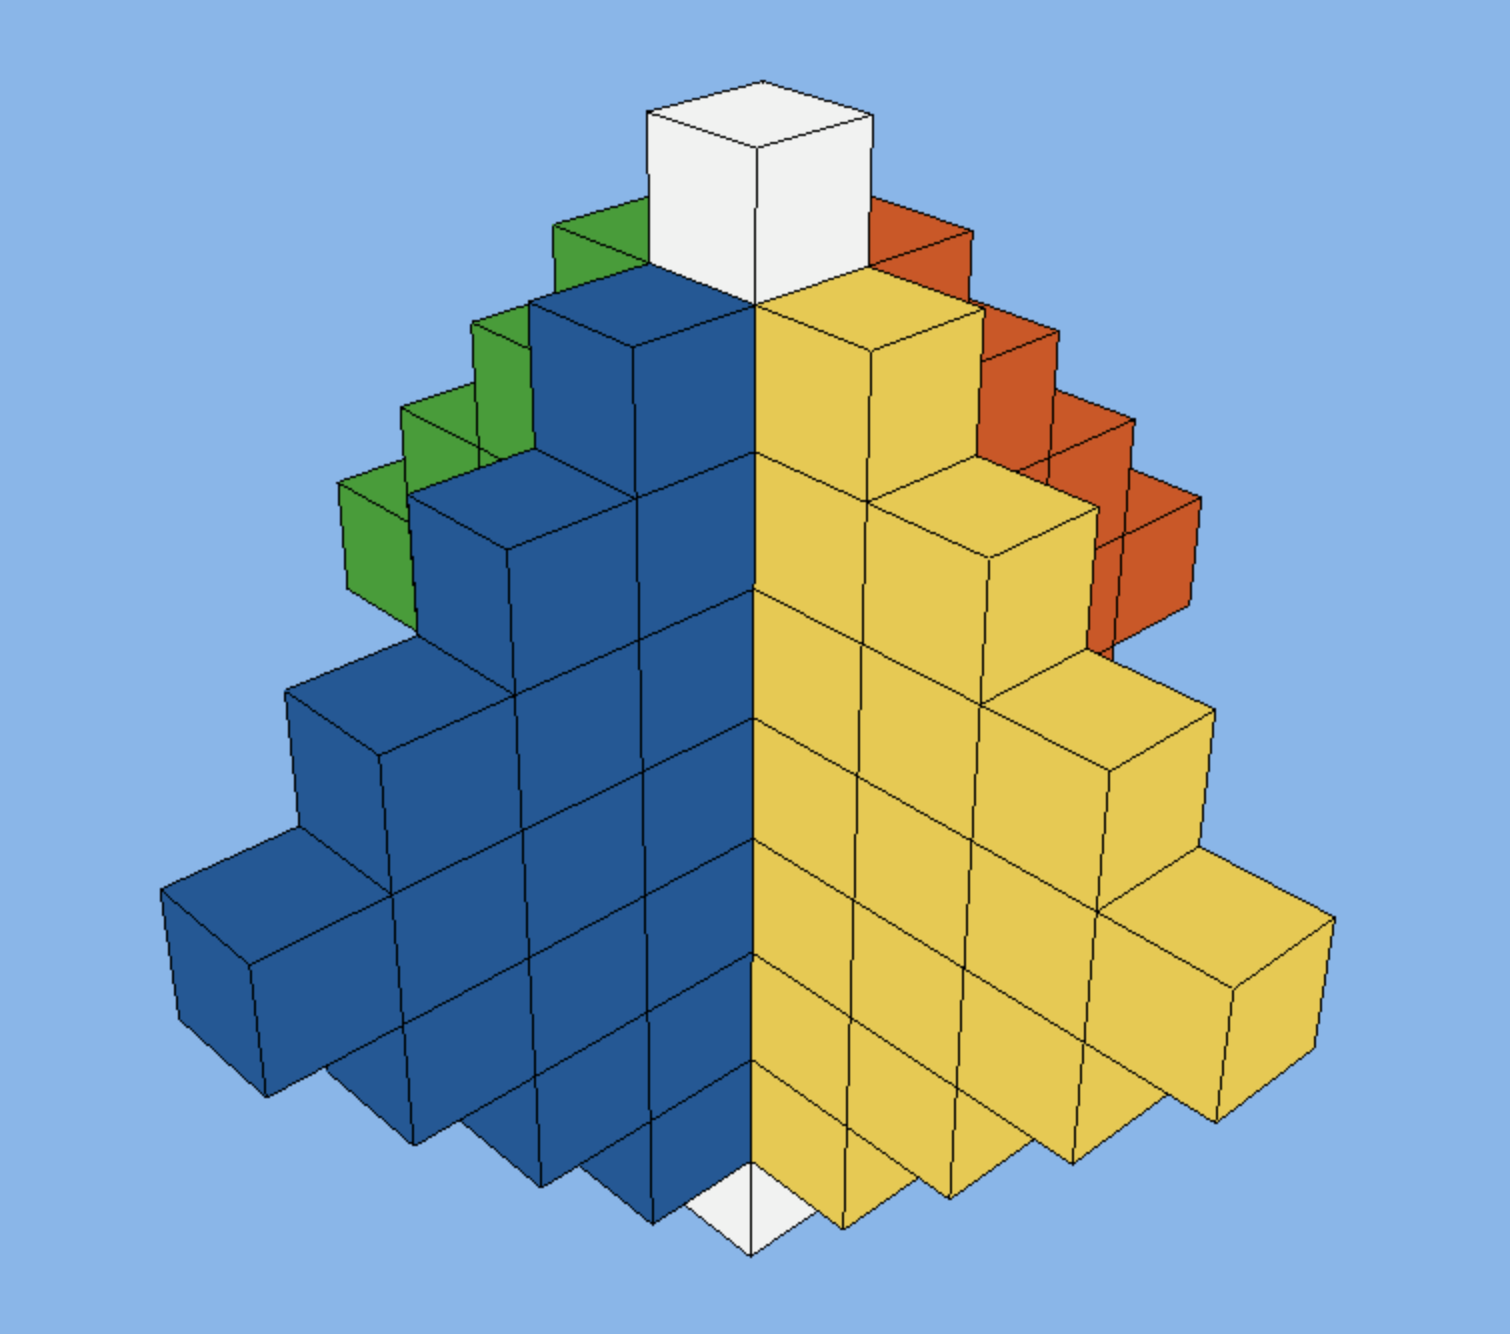
\includegraphics[height=0.1\textwidth]{../figures/angle4.png}
    \caption{Orientations of a $\bigcap_{i = 1}^4 \mathcal{L}(\mathcal{G}_i) \cap \Sigma ^6$ configuration. As $c \rightarrow \infty$, this shape approximates a circular cone whose symmetric axis joins $\sigma_i$ with orthonormal unit productions $w_i \rightarrow t_\cap$, and $S_i \in \Lambda^*_{\sigma}?$ represented by the outermost bitvector inhabitants. Equations of this form are equiexpressive with the family of CSLs realizable by finite CFL intersection.}
\end{figure}

It is a well-known fact in formal language theory that CFLs are closed under union, composition, substitution and intersection with regular languages, and the intersection between two CFLs is decidable. Anyhow, since we are working with bounded-width CFLs, everything collapses down to finite languages, which are closed under all these operations. Thus, Bar-Hillel and other elegant constructions which took CS theorists many years to prove in full-generality become trivial when so restricted.

Given two CFLs $\mathcal{L}_\mathcal{G}, \mathcal{L}_{\mathcal{G}'}$, we can compute the intersection $\mathcal{L}_\mathcal{G}\cap\mathcal{L}_{\mathcal{G}'}\cap\Sigma^d$ by encoding $(\mathbf{M}_\mathcal{G}^*\sigma) = (\mathbf{M}_{\mathcal{G}'}^*\sigma)$. This allows us to build a DSL of grammar combinators to constrain the solution space.

For example, we can solve $\Sigma^d \cap \overline{\mathcal{L}_\mathcal{G}}$ by enumerating $\{\beta\sigma'\gamma \mid \sigma' \in \Sigma^d, \beta = \gamma = \_^k\}$, overapproximating the prefix and suffix (padding left and right), and checking for UNSAT to underapproximate \textit{impossible substrings}, strings which cannot appear in any $\{\sigma \in \mathcal{L}_\mathcal{G}\}$. Precomputing impossible substrings for a given grammar allows us to quickly eliminate inadmissible repairs and localize syntax errors in candidate strings.

We can also build a set of grammars of increasing granularity, like a lattice structure. Basically, we can build up a lattice (in the order theoretic sense), consisting of grammars of increasing granularity. All programming languages require balanced parentheses, but some have additional constraints. So we can combine grammars, count and do bounded linear integer arithmetic.

\section{Coarsening and simplification of subexpressions}

Clearly, the solving process is polynomial in the size of the string. For the sake of complexity, it would be convenient if well-formed subexpressions could be collapsed into a single nonterminal, or multiple nonterminals (in case of ambiguity). Naturally, this raises the question of when can partial derivations be simplified? This transformation is admissible and indeed desirable when the subexpression is ``complete'', i.e., its derivation cannot be altered by appending or prepending text. Returning to Fig. 4, under what circumstances is the following reduction admissible?

\begin{figure}[H]
 \[
    \mathbf{M}^* = \begin{pNiceArray}{>{\strut}ccccccc}[margin, extra-margin=2pt,colortbl-like, xdots/line-style=loosely dotted]
       \vno & \rcr \vs{1} &  \mathcal{L}_{1,3} & \mathcal{L}_{1,3} & \rcw \mathcal{V}_{1,4} & \cdd & \mathcal{V}_{1,n} \\
       \vdd & \ddd        &  \rcr\vs{2}        & \mathcal{L}_{2,3} & \rcw\vdd               &      & \vdd \\
            &             &                    & \rcr\vs{3}        & \rcw                   &      & \\
            &             &                    &                   & \mathcal{V}_{4,4}      &      & \\
            &             &                    &                   &                        & \ddd & \\
            &             &                    &                   &                        &      & \mathcal{V}_{n,n} \\
       \vno & \cdd        &                    &                   &                        &      & \vno
    \end{pNiceArray} \equiv
    \begin{pNiceArray}{>{\strut}ccccc}[margin, extra-margin=2pt,colortbl-like, xdots/line-style=loosely dotted]
       \vno & \rcr\mathcal{L}_{1,3} & \rcw\mathcal{V}_{1,4} & \cdd & \mathcal{V}_{1,n} \\
       \vdd & \ddd                  & \mathcal{V}_{2,4}     &      & \vdd \\
            &                       &                       & \ddd & \\
            &                       &                       &      & \mathcal{V}_{n,n} \\
       \vno & \cdd                  &                       &      & \vno
    \end{pNiceArray}
 \]
\end{figure}

For example, the string \texttt{( - b )} is morally \textit{complete} in the sense that inserting adjacent text should not alter the interior derivation, while \texttt{- b} is not, as introducing adjacent text (e.g. \texttt{a - b}) may alter the derivation of its contents depending on the structure of the CFG. How can we formalize this argument to work on arbitrary (e.g., potentially ambiguous) grammars? This question can be reduced to a quotient: Does there exist another nonterminal, when joined with the substring in question, that will ``strip away'' any of its tokens, leading to another derivation?

\section{Realtime Error Correction}\label{sec:holes}

Now that we have a reliable method to fix \textit{localized} errors, $S: \mathcal{G} \times (\Sigma\cup\{\varepsilon, \texttt{\_}\})^n \rightarrow \{\Sigma^n\}\subseteq \mathcal{L}_\mathcal{G}$, given an input string, $\Sigma^n$, where should we put the holes? Assuming $k$ holes, there are ${n \choose k}$ possible hole configurations (HCs), each with $(|\Sigma| + 1)^{2k}$ possible repairs (before parsing, cf. Eqs.~\ref{eq:del}-\ref{eq:ins2}). In practice, depending on $n$ and $k$, this space can be intractable to search through exhaustively, so to facilitate real-time assistance we prioritize likely repairs according to an eight-step procedure:

\begin{enumerate}
    \item Fetch the most recent CFG and string from the editor.
    \item Exclude parsable substrings from hollowing.
    \item Lazily enumerate all HCs of increasing length.
    \item Sample HCs without replacement using Eq.~\ref{eq:ergo}.
    \item Prioritize HCs first by distance to caret index, then by Earthmover's distance to a set of suspicious indices.$^*$
    \item Translate HCs to sketch templates using~\S\ref{sec:dsi}.
    \item Feed sketch templates to an incremental SAT solver.
    \item Decode and rerank models by Levenshtein distance.
\end{enumerate}

\noindent $^*$ These locations can be supplied by local edit history or using tokenwise perplexity from a neural language model. Once a new repair is discovered, it is immediately displayed. Incoming keystrokes interrupt and reset the solving process.


\section{Practical Example}

Tidyparse requires a grammar -- this can be either provided by the user or ingested from a BNF-like specification. The following is a slightly more complex grammar, designed to resemble a more realistic use case:

\begin{tidyinput}
S -> A | V | ( X , X ) | X X | ( X )
A -> Fun | F | L | L in X
Fun -> fun V (*@`@*)->(*@`@*) X
F -> if X then X else X
L -> let V = X | let rec V = X
V -> Vexp | ( Vexp ) | Vexp Vexp
Vexp -> VarName | FunName | Vexp VO Vexp
Vexp -> ( VarName , VarName ) | Vexp Vexp
VarName -> a | b | c | d | e | ... | z
FunName -> foldright | map | filter
VO ->  + | - | * | / | > | = | < | (*@`@*)||(*@`@*) | &&
---
let curry f = ( fun x y -> f ( _ _ _(*@\caret{ }@*)) )
\end{tidyinput}
\begin{tidyoutput}
let curry f = ( fun x y -> f ( (*@\hlorange{<X>}@*) ) )
let curry f = ( fun x y -> f ( (*@\hlorange{<FunName>}@*) ) )
let curry f = ( fun x y -> f ( (*@\hlorange{curry}@*) (*@\hlorange{<X>}@*) ) )
...
\end{tidyoutput}

\subsection{Grammar Assistance}

Tidyparse uses a CFG to parse the CFG, so it can provide assistance while the user is designing the CFG. For example, if the CFG does not parse, it will suggest possible fixes. In the future, we intend to use this functionality to perform example-based codesign and grammar induction.

\begin{tidyinput}
B -> true | false | (*@\caret{ }@*)
\end{tidyinput}
\begin{tidyoutput}
B -> true | false (*@\hlred{ }@*)
B -> true | false (*@\hlorange{<RHS>}@*)
B -> true | false | (*@\hlgreen{<RHS>}@*)
...
\end{tidyoutput}

\subsection{Interactive Nonterminal Expansion}

Users can interactively build up a complex expression by placing the caret over a placeholder they wish to expand,

\begin{tidyinput}
if <(*@\caret{V}@*)exp> X then <Vexp> else <Vexp>
\end{tidyinput}

\noindent then invoking Tidyparse by pressing \keys{\ctrl + \SPACE}, to receive a list of expressions consistient with the grammar:

\begin{tidyoutput}
if (*@\hlorange{map}@*) X then <Vexp> else <Vexp>
if (*@\hlorange{uncurry}@*) X then <Vexp> else <Vexp>
if (*@\hlorange{foldright}@*) X then <Vexp> else <Vexp>
...
\end{tidyoutput}

%There are some more examples too.
%
%The line between parsing and computation is blurry.


\section{Evaluation}

In the following benchmarks, we measure the wall clock time required to synthesize solutions to length-50 strings sampled from various Dyck languages, where Dyck-n is the Dyck language containing n types of balanced parentheses.

\begin{tidyinput}
D1 -> () | ( D1 ) | D1 D1
D2 -> D1 | [ ] | ( D2 ) | [ D2 ] | D2 D2
D3 -> D2 | { } | ( D3 ) | [ D3 ] | { D3 } | D3 D3
\end{tidyinput}

\noindent In the first experiment, we sample a random valid string $\sigma \sim \Sigma^{50} \cap \mathcal{L}_{\text{Dyck-n}}$, then replace a fixed number tokens with holes and measure the average time taken to decode ten syntactically-admissible repairs across 100 trial runs.

\begin{tikzpicture}
    \begin{axis}[
        width=8.3cm,
        title={\hspace{-1cm}\textbf{Error correction time with known locations}},
        ybar,
        bar width=4pt,
        xlabel={Number of holes},
        ylabel={ms to synthesize 10 repairs},
        xtick=data,
        axis x line*=bottom,
        axis y line*=left,
        ytick pos=left,
        xticklabels from table={\loctimings}{holes},
        ymajorgrids,
        legend pos=north west,
        error bars/y dir=both,
        error bars/y explicit
    ]
    \addplot table [x expr=\coordindex, y=d1, y error=d1err]{\loctimings};
    \addplot table [x expr=\coordindex, y=d2, y error=d2err]{\loctimings};
    \addplot table [x expr=\coordindex, y=d3, y error=d3err]{\loctimings};
    \addplot table [x expr=\coordindex, y=d4, y error=d4err]{\loctimings};
    \legend{Dyck-1, Dyck-2, Dyck-3, Dyck-4}
    \end{axis}
\end{tikzpicture}

\noindent In the second experiment, we sample a random valid string as before, but delete p tokens at random and rather than provide the location(s), ask our model to solve for both the location(s) and repair by sampling uniformly from all n-token HCs, then measure the total time required to decode the first admissible repair. Note the the logarithmic scale on the y-axis.

\begin{tikzpicture}
    \begin{axis}[
        width=8.3cm,
        height=6.6cm,
        title={\hspace{-1cm}\textbf{Error correction time with unknown locations}},
        ybar,
        bar width=20pt,
        xlabel={Number of errors},
        ylabel={ms to synthesize 1 repair},
        xtick=data,
        axis x line*=bottom,
        axis y line*=left,
        enlarge x limits={abs=0.5},
        ymode=log,
        ytick pos=left,
        xticklabels from table={\unloctimings}{errors},
        ymajorgrids,
        legend pos=north west,
        error bars/y dir=both,
        error bars/y explicit
    ]
    \addplot table [x expr=\coordindex, y=d1]{\unloctimings};
    \addplot table [x expr=\coordindex, y=d2]{\unloctimings};
    \addplot table [x expr=\coordindex, y=d3]{\unloctimings};
    \legend{Dyck-1, Dyck-2, Dyck-3}
    \end{axis}
\end{tikzpicture}

\subsection{Task Difficulty}

\noindent\textbf{Level \textonehalf} - Incomplete code (all missing tokens at end)

\noindent\textbf{Level 1} - Known number of errors at known locations

\noindent\textbf{Level 2} - Known number of errors at unknown locations

\noindent\textbf{Level 3} - Unknown number of errors at unknown locations

\subsection{Repair Datasets}
Synthetic - Synthetic errors in natural code snippets\\
Natural - Natural errors and fixes mined from Git history
\subsection{Evaluation Metrics}
Syntactic validity - Only considers whether the repair parses\\
Repair alignment - Measures string distance to true fix
\subsection{Model configurations}
Model configurations - LLM, ECP, ECP + LLM
GraphCodeBERT
RobertA
Incoder
CarperAI?

\section{Discussion}

While error correction with a few errors is tolerable, latency can vary depending on many factors including string length and grammar size. If errors are known to be concentrated in specific locations, such as the beginning or end of a string, then latency is typically below 500ms. Should errors occur uniformly at random, admissible repairs can take longer to discover, however these scenarios are unusual in our experience. We observe that errors are typically concentrated nearby historical edit locations, which can be retrieved from the IDE or version control. Further optimizations that reduce the total number of repairs checked are possible by eliminating improbable sketch templates.

Tidyparse in its current form has a number of technical shortcomings: firstly it does not incorporate any neural language modeling technology at present, an omission we hope to address in the near future. Training a language model to predict likely repair locations and rank admissible results could lead to lower overall latency and more natural repairs.

Secondly, our current method generates sketch templates using a na\"ive enumerative search, feeding them individually to the SAT solver, which has the tendency to duplicate prior work and introduces unnecessary thrashing. Considering recent extensions of Boolean matrix-based parsing to linear context-free rewriting systems (LCFRS)~\cite{cohen2016parsing}, it may be feasible to search through these edits within the SAT solver, leading to yet unrealized and possibly significant speedups.

Lastly and perhaps most significantly, Tidyparse does not incorporate any semantic constraints, so its repairs while syntactically admissible, are not guaranteed to be semantically valid. We note however, that it is possible to encode type-based semantic constraints into the solver and intend to explore this direction more fully in future work.

Although not intended to be a dedicated parser and we make no attempt to rigorously compare parsing latency, parsing valid strings with Tidyparse is typically competitive with classical parsing methods. Our primary motivation is to facilitate the usability and explainability of parsing with errors. We envision three primary use cases: (1) helping novice programmers become more quickly familiar with a new programming language (2) autocorrecting common typos among proficient but forgetful programmers and (3) as a prototyping tool for PL educators and designers.

Featuring a grammar editor and built-in SAT solver, Tidyparse helps developers navigate the language design space, visualize syntax trees, debug parsing errors and quickly generate simple examples and counterexamples for testing. Although the algorithm may seem esoteric at first glance, in our experience it is much more interpretable than classical parsers, which exhibit poor error-recovery and diagnostics.

\section{Conclusion}

Tidyparse accepts a CFG and a string to parse. If the string is valid, it returns the parse forest, otherwise, it returns a set of repairs, ordered by their Levenshtein edit distance to the invalid string. Our method compiles each CFG and candidate string onto a matrix dynamical system using an extended version of Valiant's construction and solves for its fixedpoints using an incremental SAT solver. This approach to parsing has many advantages, enabling us to repair syntax errors, correct typos and generate parse trees for incomplete strings. By allowing the string to contain holes, repairs can contain either concrete tokens or nonterminals, which can be manually expanded by the user or a neural-guided search procedure. From a theoretical standpoint, this technique is particularly amenable to neural program synthesis and repair, naturally integrating with the masked-language-modeling task (MLM) used by transformer-based neural language models.

From a practical standpoint, we have implemented our approach as an IDE plugin and demonstrated its viability as a tool for live programming. Tidyparse is capable of generating repairs for invalid code in a range of toy languages. We plan to continue expanding its grammar and autocorrection functionality to cover a broader range of languages and hope to conduct a more thorough user study to validate its effectiveness in the near future. %Further examples can be found at our GitHub repository: \url{https://github.com/breandan/tidyparse} (needs anonymiziation)

%\begin{itemize}
%\item Error correction.
%\item Program repair.
%\item Program synthesis.
%\item Parsing with holes.
%\item Naturally integrates with masked language model (MLM)-based neural program repair.
%\item Parsing with natural error recovery.
%\item Helps to facilitate language learning.
%\item GPU acceleration.
%\end{itemize}

\bibliography{../bib/acmart}

\appendix

\section{Example Repairs}
\begin{figure}[H]
  \begin{center}
    \begin{tabular}{|p{5cm}|p{5cm}|}
      \hline\\[-1em]1.a) Original method  &  1.b) Synonymous variant\\[-1em]\\\hline
      \begin{lstlisting}[basicstyle=\ttfamily\lst@ifdisplaystyle\footnotesize\fi, language=kotlin]
public void flush(int b) {
    buffer.write((byte) b);
    buffer.compact();
}
      \end{lstlisting} & \begin{lstlisting}[basicstyle=\ttfamily\lst@ifdisplaystyle\footnotesize\fi, language=kotlin]
public void flush(int b) {
    (*@\hlred{cushion}@*).write((byte) b);
    (*@\hlred{cushion}@*).compact();
}
      \end{lstlisting}
      \\\hline\\[-1em]2.a) Multi-masked method   &  2.b) Multi-masked variant\\[-1em]\\\hline
      \begin{lstlisting}[basicstyle=\ttfamily\lst@ifdisplaystyle\footnotesize\fi, language=kotlin]
public void <MASK>(int b) {
    buffer.<MASK>((byte) b);
    <MASK>.compact();
}
      \end{lstlisting} & \begin{lstlisting}[basicstyle=\ttfamily\lst@ifdisplaystyle\footnotesize\fi, language=kotlin]
public void <MASK>(int b) {
    cushion.<MASK>((byte) b);
    <MASK>.compact();
}
      \end{lstlisting}
      \\\hline\\[-1em]3.a) Model predictions  &  3.b) Model predictions\\[-1em]\\\hline
      \begin{lstlisting}[basicstyle=\ttfamily\lst@ifdisplaystyle\footnotesize\fi, language=kotlin]
public void (*@\hl{output}@*)(int b) {
    buffer.write((byte) b);
    buffer.compact();
}
      \end{lstlisting} & \begin{lstlisting}[basicstyle=\ttfamily\lst@ifdisplaystyle\footnotesize\fi, language=kotlin]
public void (*@\hl{append}@*)(int b) {
    cushion.(*@\hl{add}@*)((byte) b);
    cushion.compact();
}
      \end{lstlisting} \\\hline
    \end{tabular}
  \end{center}
\end{figure}
\end{document}